% ======================================================================
% paper_merged.tex — single-document SPDE-AC-shaped working paper
% (BENCHMARK_ANALYSIS.md §5 blueprint: statements first, one proofs
% section containing parts S0–S8 with the v2 closures, applications and
% numerics after the proofs, numeric bibliography.)
% Build: python3 build_supplement.py
%        pdflatex paper_merged && bibtex paper_merged && pdflatex x2
% ======================================================================
\documentclass[10pt]{article}
\newcommand{\MERGEDDOC}{}          % toggles merged-aware wording in sections/
\usepackage[a4paper,margin=0.9in]{geometry}
\usepackage[T1]{fontenc}
\usepackage[utf8]{inputenc}
\usepackage{lmodern}
\usepackage{microtype}
\usepackage{amsmath,amssymb,amsthm,mathtools,bm}
\usepackage{booktabs,tabularx,array,longtable}
\usepackage{graphicx}
\usepackage[font=small]{caption}
\usepackage{subcaption}
\usepackage{xcolor,float}
\usepackage{enumitem}
\usepackage[numbers,sort&compress]{natbib}
\setlength{\bibsep}{2.5pt}
\renewcommand{\bibfont}{\small}
\usepackage{pifont}
\usepackage{tikz}
\usetikzlibrary{arrows.meta,positioning,calc,shapes.geometric,fit,backgrounds,matrix,shapes.misc,decorations.pathreplacing}
\graphicspath{{figures/}{wp_figures/}}
\usepackage{hyperref}
\usepackage[capitalise]{cleveref}
\hypersetup{colorlinks=true,linkcolor=blue!55!black,citecolor=blue!55!black,urlcolor=blue!55!black}

% compact spacing (submission-length calibration)
\AtBeginDocument{%
 \setlength{\abovedisplayskip}{5pt plus 1pt minus 2pt}%
 \setlength{\belowdisplayskip}{5pt plus 1pt minus 2pt}%
 \setlength{\abovedisplayshortskip}{2pt plus 1pt}%
 \setlength{\belowdisplayshortskip}{3pt plus 1pt}%
 \setlength{\textfloatsep}{11pt plus 2pt minus 2pt}%
 \setlength{\abovecaptionskip}{5pt}}
\setlist{itemsep=1pt, topsep=3pt, parsep=0pt}
\makeatletter
\def\thm@space@setup{\thm@preskip=6pt \thm@postskip=6pt}
\makeatother
\usepackage{titlesec}
\titlespacing*{\section}{0pt}{14pt plus 3pt minus 3pt}{7pt plus 2pt}
\titlespacing*{\subsection}{0pt}{11pt plus 3pt minus 2pt}{5pt plus 2pt}
\titlespacing*{\subsubsection}{0pt}{9pt plus 2pt minus 2pt}{4pt plus 1pt}

\newtheorem{definition}{Definition}[section]
\newtheorem{assumption}{Assumption}[section]
\newtheorem{theorem}{Theorem}[section]
\newtheorem{proposition}{Proposition}[section]
\newtheorem{lemma}{Lemma}[section]
\newtheorem{corollary}{Corollary}[section]
\theoremstyle{remark}
\newtheorem{remark}{Remark}[section]
\newtheorem{example}{Example}[section]
\crefname{assumption}{Assumption}{Assumptions}
\Crefname{assumption}{Assumption}{Assumptions}

% ---- main-text macros ----
\newcommand{\R}{\mathbb R}
\newcommand{\N}{\mathbb N}
\newcommand{\E}{\mathbb E}
\newcommand{\Pp}{\mathbb P}
\newcommand{\Law}{\mathcal L}
\newcommand{\cT}{\mathcal T}
\newcommand{\cW}{\mathcal W}
\newcommand{\cZ}{\mathcal Z}
\newcommand{\cO}{\mathcal O}
\newcommand{\cM}{\mathfrak M}
\newcommand{\cI}{\mathcal I}
\newcommand{\Var}{\operatorname{Var}}
\newcommand{\Cov}{\operatorname{Cov}}
\newcommand{\diag}{\operatorname{diag}}
\newcommand{\doop}{\operatorname{do}}
\newcommand{\op}{o_{\Pp}}
\newcommand{\Op}{O_{\Pp}}
\newcommand{\norm}[1]{\left\lVert#1\right\rVert}
\newcommand{\abs}[1]{\left\lvert#1\right\rvert}
\newcommand{\inner}[2]{\left\langle#1,#2\right\rangle}
\newcommand{\cf}{\mathrm{cf}}
\newcommand{\fact}{\mathrm{fact}}
\newcommand{\inwords}[1]{\par\smallskip\noindent\textit{Interpretation.} #1\par\smallskip}
\newcommand{\yes}{\textcolor{green!55!black}{\ding{51}}}
\newcommand{\no}{\textcolor{red!70!black}{\ding{55}}}
\newcommand{\half}{\textcolor{orange!85!black}{$\displaystyle\sim$}}

% ---- fallbacks for the proofs parts (parts re-define group-locally) ----
\providecommand{\LamN}{\Lambda_N}
\providecommand{\An}{A_{N,n}}
\providecommand{\Dn}{D_{N,n}}
\providecommand{\Dmat}{D_{N,n}}
\providecommand{\vart}{\vartheta}
\providecommand{\vzero}{\vartheta_0}
\providecommand{\vhat}{\widehat\vartheta_{N,n}}
\providecommand{\elln}{\ell_{N,n}}
\providecommand{\an}{a_{N,n}}
\providecommand{\bn}{b_{N,n}}
\providecommand{\cC}{\mathcal C}
\providecommand{\cG}{\mathcal G}
\providecommand{\cU}{\mathcal U}
\providecommand{\Jhat}{\widehat J_{N,n}}
\providecommand{\1}{\mathbf 1}

% Draft build: visible verification flags. Submission build: compile with
%   pdflatex "\def\SUBMISSIONCLEAN{}% ======================================================================
% paper_merged.tex — single-document SPDE-AC-shaped working paper
% (BENCHMARK_ANALYSIS.md §5 blueprint: statements first, one proofs
% section containing parts S0–S8 with the v2 closures, applications and
% numerics after the proofs, numeric bibliography.)
% Build: python3 build_supplement.py
%        pdflatex paper_merged && bibtex paper_merged && pdflatex x2
% ======================================================================
\documentclass[10pt]{article}
\newcommand{\MERGEDDOC}{}          % toggles merged-aware wording in sections/
\usepackage[a4paper,margin=0.9in]{geometry}
\usepackage[T1]{fontenc}
\usepackage[utf8]{inputenc}
\usepackage{lmodern}
\usepackage{microtype}
\usepackage{amsmath,amssymb,amsthm,mathtools,bm}
\usepackage{booktabs,tabularx,array,longtable}
\usepackage{graphicx}
\usepackage[font=small]{caption}
\usepackage{subcaption}
\usepackage{xcolor,float}
\usepackage{enumitem}
\usepackage[numbers,sort&compress]{natbib}
\setlength{\bibsep}{2.5pt}
\renewcommand{\bibfont}{\small}
\usepackage{pifont}
\usepackage{tikz}
\usetikzlibrary{arrows.meta,positioning,calc,shapes.geometric,fit,backgrounds,matrix,shapes.misc,decorations.pathreplacing}
\graphicspath{{figures/}{wp_figures/}}
\usepackage{hyperref}
\usepackage[capitalise]{cleveref}
\hypersetup{colorlinks=true,linkcolor=blue!55!black,citecolor=blue!55!black,urlcolor=blue!55!black}

% compact spacing (submission-length calibration)
\AtBeginDocument{%
 \setlength{\abovedisplayskip}{5pt plus 1pt minus 2pt}%
 \setlength{\belowdisplayskip}{5pt plus 1pt minus 2pt}%
 \setlength{\abovedisplayshortskip}{2pt plus 1pt}%
 \setlength{\belowdisplayshortskip}{3pt plus 1pt}%
 \setlength{\textfloatsep}{11pt plus 2pt minus 2pt}%
 \setlength{\abovecaptionskip}{5pt}}
\setlist{itemsep=1pt, topsep=3pt, parsep=0pt}
\makeatletter
\def\thm@space@setup{\thm@preskip=6pt \thm@postskip=6pt}
\makeatother
\usepackage{titlesec}
\titlespacing*{\section}{0pt}{14pt plus 3pt minus 3pt}{7pt plus 2pt}
\titlespacing*{\subsection}{0pt}{11pt plus 3pt minus 2pt}{5pt plus 2pt}
\titlespacing*{\subsubsection}{0pt}{9pt plus 2pt minus 2pt}{4pt plus 1pt}

\newtheorem{definition}{Definition}[section]
\newtheorem{assumption}{Assumption}[section]
\newtheorem{theorem}{Theorem}[section]
\newtheorem{proposition}{Proposition}[section]
\newtheorem{lemma}{Lemma}[section]
\newtheorem{corollary}{Corollary}[section]
\theoremstyle{remark}
\newtheorem{remark}{Remark}[section]
\newtheorem{example}{Example}[section]
\crefname{assumption}{Assumption}{Assumptions}
\Crefname{assumption}{Assumption}{Assumptions}

% ---- main-text macros ----
\newcommand{\R}{\mathbb R}
\newcommand{\N}{\mathbb N}
\newcommand{\E}{\mathbb E}
\newcommand{\Pp}{\mathbb P}
\newcommand{\Law}{\mathcal L}
\newcommand{\cT}{\mathcal T}
\newcommand{\cW}{\mathcal W}
\newcommand{\cZ}{\mathcal Z}
\newcommand{\cO}{\mathcal O}
\newcommand{\cM}{\mathfrak M}
\newcommand{\cI}{\mathcal I}
\newcommand{\Var}{\operatorname{Var}}
\newcommand{\Cov}{\operatorname{Cov}}
\newcommand{\diag}{\operatorname{diag}}
\newcommand{\doop}{\operatorname{do}}
\newcommand{\op}{o_{\Pp}}
\newcommand{\Op}{O_{\Pp}}
\newcommand{\norm}[1]{\left\lVert#1\right\rVert}
\newcommand{\abs}[1]{\left\lvert#1\right\rvert}
\newcommand{\inner}[2]{\left\langle#1,#2\right\rangle}
\newcommand{\cf}{\mathrm{cf}}
\newcommand{\fact}{\mathrm{fact}}
\newcommand{\inwords}[1]{\par\smallskip\noindent\textit{Interpretation.} #1\par\smallskip}
\newcommand{\yes}{\textcolor{green!55!black}{\ding{51}}}
\newcommand{\no}{\textcolor{red!70!black}{\ding{55}}}
\newcommand{\half}{\textcolor{orange!85!black}{$\displaystyle\sim$}}

% ---- fallbacks for the proofs parts (parts re-define group-locally) ----
\providecommand{\LamN}{\Lambda_N}
\providecommand{\An}{A_{N,n}}
\providecommand{\Dn}{D_{N,n}}
\providecommand{\Dmat}{D_{N,n}}
\providecommand{\vart}{\vartheta}
\providecommand{\vzero}{\vartheta_0}
\providecommand{\vhat}{\widehat\vartheta_{N,n}}
\providecommand{\elln}{\ell_{N,n}}
\providecommand{\an}{a_{N,n}}
\providecommand{\bn}{b_{N,n}}
\providecommand{\cC}{\mathcal C}
\providecommand{\cG}{\mathcal G}
\providecommand{\cU}{\mathcal U}
\providecommand{\Jhat}{\widehat J_{N,n}}
\providecommand{\1}{\mathbf 1}

% Draft build: visible verification flags. Submission build: compile with
%   pdflatex "\def\SUBMISSIONCLEAN{}% ======================================================================
% paper_merged.tex — single-document SPDE-AC-shaped working paper
% (BENCHMARK_ANALYSIS.md §5 blueprint: statements first, one proofs
% section containing parts S0–S8 with the v2 closures, applications and
% numerics after the proofs, numeric bibliography.)
% Build: python3 build_supplement.py
%        pdflatex paper_merged && bibtex paper_merged && pdflatex x2
% ======================================================================
\documentclass[10pt]{article}
\newcommand{\MERGEDDOC}{}          % toggles merged-aware wording in sections/
\usepackage[a4paper,margin=0.9in]{geometry}
\usepackage[T1]{fontenc}
\usepackage[utf8]{inputenc}
\usepackage{lmodern}
\usepackage{microtype}
\usepackage{amsmath,amssymb,amsthm,mathtools,bm}
\usepackage{booktabs,tabularx,array,longtable}
\usepackage{graphicx}
\usepackage[font=small]{caption}
\usepackage{subcaption}
\usepackage{xcolor,float}
\usepackage{enumitem}
\usepackage[numbers,sort&compress]{natbib}
\setlength{\bibsep}{2.5pt}
\renewcommand{\bibfont}{\small}
\usepackage{pifont}
\usepackage{tikz}
\usetikzlibrary{arrows.meta,positioning,calc,shapes.geometric,fit,backgrounds,matrix,shapes.misc,decorations.pathreplacing}
\graphicspath{{figures/}{wp_figures/}}
\usepackage{hyperref}
\usepackage[capitalise]{cleveref}
\hypersetup{colorlinks=true,linkcolor=blue!55!black,citecolor=blue!55!black,urlcolor=blue!55!black}

% compact spacing (submission-length calibration)
\AtBeginDocument{%
 \setlength{\abovedisplayskip}{5pt plus 1pt minus 2pt}%
 \setlength{\belowdisplayskip}{5pt plus 1pt minus 2pt}%
 \setlength{\abovedisplayshortskip}{2pt plus 1pt}%
 \setlength{\belowdisplayshortskip}{3pt plus 1pt}%
 \setlength{\textfloatsep}{11pt plus 2pt minus 2pt}%
 \setlength{\abovecaptionskip}{5pt}}
\setlist{itemsep=1pt, topsep=3pt, parsep=0pt}
\makeatletter
\def\thm@space@setup{\thm@preskip=6pt \thm@postskip=6pt}
\makeatother
\usepackage{titlesec}
\titlespacing*{\section}{0pt}{14pt plus 3pt minus 3pt}{7pt plus 2pt}
\titlespacing*{\subsection}{0pt}{11pt plus 3pt minus 2pt}{5pt plus 2pt}
\titlespacing*{\subsubsection}{0pt}{9pt plus 2pt minus 2pt}{4pt plus 1pt}

\newtheorem{definition}{Definition}[section]
\newtheorem{assumption}{Assumption}[section]
\newtheorem{theorem}{Theorem}[section]
\newtheorem{proposition}{Proposition}[section]
\newtheorem{lemma}{Lemma}[section]
\newtheorem{corollary}{Corollary}[section]
\theoremstyle{remark}
\newtheorem{remark}{Remark}[section]
\newtheorem{example}{Example}[section]
\crefname{assumption}{Assumption}{Assumptions}
\Crefname{assumption}{Assumption}{Assumptions}

% ---- main-text macros ----
\newcommand{\R}{\mathbb R}
\newcommand{\N}{\mathbb N}
\newcommand{\E}{\mathbb E}
\newcommand{\Pp}{\mathbb P}
\newcommand{\Law}{\mathcal L}
\newcommand{\cT}{\mathcal T}
\newcommand{\cW}{\mathcal W}
\newcommand{\cZ}{\mathcal Z}
\newcommand{\cO}{\mathcal O}
\newcommand{\cM}{\mathfrak M}
\newcommand{\cI}{\mathcal I}
\newcommand{\Var}{\operatorname{Var}}
\newcommand{\Cov}{\operatorname{Cov}}
\newcommand{\diag}{\operatorname{diag}}
\newcommand{\doop}{\operatorname{do}}
\newcommand{\op}{o_{\Pp}}
\newcommand{\Op}{O_{\Pp}}
\newcommand{\norm}[1]{\left\lVert#1\right\rVert}
\newcommand{\abs}[1]{\left\lvert#1\right\rvert}
\newcommand{\inner}[2]{\left\langle#1,#2\right\rangle}
\newcommand{\cf}{\mathrm{cf}}
\newcommand{\fact}{\mathrm{fact}}
\newcommand{\inwords}[1]{\par\smallskip\noindent\textit{Interpretation.} #1\par\smallskip}
\newcommand{\yes}{\textcolor{green!55!black}{\ding{51}}}
\newcommand{\no}{\textcolor{red!70!black}{\ding{55}}}
\newcommand{\half}{\textcolor{orange!85!black}{$\displaystyle\sim$}}

% ---- fallbacks for the proofs parts (parts re-define group-locally) ----
\providecommand{\LamN}{\Lambda_N}
\providecommand{\An}{A_{N,n}}
\providecommand{\Dn}{D_{N,n}}
\providecommand{\Dmat}{D_{N,n}}
\providecommand{\vart}{\vartheta}
\providecommand{\vzero}{\vartheta_0}
\providecommand{\vhat}{\widehat\vartheta_{N,n}}
\providecommand{\elln}{\ell_{N,n}}
\providecommand{\an}{a_{N,n}}
\providecommand{\bn}{b_{N,n}}
\providecommand{\cC}{\mathcal C}
\providecommand{\cG}{\mathcal G}
\providecommand{\cU}{\mathcal U}
\providecommand{\Jhat}{\widehat J_{N,n}}
\providecommand{\1}{\mathbf 1}

% Draft build: visible verification flags. Submission build: compile with
%   pdflatex "\def\SUBMISSIONCLEAN{}% ======================================================================
% paper_merged.tex — single-document SPDE-AC-shaped working paper
% (BENCHMARK_ANALYSIS.md §5 blueprint: statements first, one proofs
% section containing parts S0–S8 with the v2 closures, applications and
% numerics after the proofs, numeric bibliography.)
% Build: python3 build_supplement.py
%        pdflatex paper_merged && bibtex paper_merged && pdflatex x2
% ======================================================================
\documentclass[10pt]{article}
\newcommand{\MERGEDDOC}{}          % toggles merged-aware wording in sections/
\usepackage[a4paper,margin=0.9in]{geometry}
\usepackage[T1]{fontenc}
\usepackage[utf8]{inputenc}
\usepackage{lmodern}
\usepackage{microtype}
\usepackage{amsmath,amssymb,amsthm,mathtools,bm}
\usepackage{booktabs,tabularx,array,longtable}
\usepackage{graphicx}
\usepackage[font=small]{caption}
\usepackage{subcaption}
\usepackage{xcolor,float}
\usepackage{enumitem}
\usepackage[numbers,sort&compress]{natbib}
\setlength{\bibsep}{2.5pt}
\renewcommand{\bibfont}{\small}
\usepackage{pifont}
\usepackage{tikz}
\usetikzlibrary{arrows.meta,positioning,calc,shapes.geometric,fit,backgrounds,matrix,shapes.misc,decorations.pathreplacing}
\graphicspath{{figures/}{wp_figures/}}
\usepackage{hyperref}
\usepackage[capitalise]{cleveref}
\hypersetup{colorlinks=true,linkcolor=blue!55!black,citecolor=blue!55!black,urlcolor=blue!55!black}

% compact spacing (submission-length calibration)
\AtBeginDocument{%
 \setlength{\abovedisplayskip}{5pt plus 1pt minus 2pt}%
 \setlength{\belowdisplayskip}{5pt plus 1pt minus 2pt}%
 \setlength{\abovedisplayshortskip}{2pt plus 1pt}%
 \setlength{\belowdisplayshortskip}{3pt plus 1pt}%
 \setlength{\textfloatsep}{11pt plus 2pt minus 2pt}%
 \setlength{\abovecaptionskip}{5pt}}
\setlist{itemsep=1pt, topsep=3pt, parsep=0pt}
\makeatletter
\def\thm@space@setup{\thm@preskip=6pt \thm@postskip=6pt}
\makeatother
\usepackage{titlesec}
\titlespacing*{\section}{0pt}{14pt plus 3pt minus 3pt}{7pt plus 2pt}
\titlespacing*{\subsection}{0pt}{11pt plus 3pt minus 2pt}{5pt plus 2pt}
\titlespacing*{\subsubsection}{0pt}{9pt plus 2pt minus 2pt}{4pt plus 1pt}

\newtheorem{definition}{Definition}[section]
\newtheorem{assumption}{Assumption}[section]
\newtheorem{theorem}{Theorem}[section]
\newtheorem{proposition}{Proposition}[section]
\newtheorem{lemma}{Lemma}[section]
\newtheorem{corollary}{Corollary}[section]
\theoremstyle{remark}
\newtheorem{remark}{Remark}[section]
\newtheorem{example}{Example}[section]
\crefname{assumption}{Assumption}{Assumptions}
\Crefname{assumption}{Assumption}{Assumptions}

% ---- main-text macros ----
\newcommand{\R}{\mathbb R}
\newcommand{\N}{\mathbb N}
\newcommand{\E}{\mathbb E}
\newcommand{\Pp}{\mathbb P}
\newcommand{\Law}{\mathcal L}
\newcommand{\cT}{\mathcal T}
\newcommand{\cW}{\mathcal W}
\newcommand{\cZ}{\mathcal Z}
\newcommand{\cO}{\mathcal O}
\newcommand{\cM}{\mathfrak M}
\newcommand{\cI}{\mathcal I}
\newcommand{\Var}{\operatorname{Var}}
\newcommand{\Cov}{\operatorname{Cov}}
\newcommand{\diag}{\operatorname{diag}}
\newcommand{\doop}{\operatorname{do}}
\newcommand{\op}{o_{\Pp}}
\newcommand{\Op}{O_{\Pp}}
\newcommand{\norm}[1]{\left\lVert#1\right\rVert}
\newcommand{\abs}[1]{\left\lvert#1\right\rvert}
\newcommand{\inner}[2]{\left\langle#1,#2\right\rangle}
\newcommand{\cf}{\mathrm{cf}}
\newcommand{\fact}{\mathrm{fact}}
\newcommand{\inwords}[1]{\par\smallskip\noindent\textit{Interpretation.} #1\par\smallskip}
\newcommand{\yes}{\textcolor{green!55!black}{\ding{51}}}
\newcommand{\no}{\textcolor{red!70!black}{\ding{55}}}
\newcommand{\half}{\textcolor{orange!85!black}{$\displaystyle\sim$}}

% ---- fallbacks for the proofs parts (parts re-define group-locally) ----
\providecommand{\LamN}{\Lambda_N}
\providecommand{\An}{A_{N,n}}
\providecommand{\Dn}{D_{N,n}}
\providecommand{\Dmat}{D_{N,n}}
\providecommand{\vart}{\vartheta}
\providecommand{\vzero}{\vartheta_0}
\providecommand{\vhat}{\widehat\vartheta_{N,n}}
\providecommand{\elln}{\ell_{N,n}}
\providecommand{\an}{a_{N,n}}
\providecommand{\bn}{b_{N,n}}
\providecommand{\cC}{\mathcal C}
\providecommand{\cG}{\mathcal G}
\providecommand{\cU}{\mathcal U}
\providecommand{\Jhat}{\widehat J_{N,n}}
\providecommand{\1}{\mathbf 1}

% Draft build: visible verification flags. Submission build: compile with
%   pdflatex "\def\SUBMISSIONCLEAN{}\input{paper_merged}"
% which silences the flags (status tracked in CHANGES_v2.md).
\ifdefined\SUBMISSIONCLEAN
\newcommand{\closuredraft}{}
\else
\newcommand{\closuredraft}{\par\smallskip\noindent
\textcolor{blue!55!black}{\footnotesize\textbf{[Verification
pending.]}}\par\smallskip}
\fi

\title{\textbf{Operator Interventions in Linear SPDEs:\\
Galerkin Structural Semantics, Mixed-Rate Local Asymptotic Normality,\\
and Uniform Inference for Post-Intervention Laws}}
\author{Gabriel Lucas St\'ephane Bontemps\thanks{Email:
\texttt{[address]}. ORCID: \texttt{[id]}.}\\[2pt]
{\normalsize GREDEG--CNRS, Universit\'e C\^ote d'Azur, Nice, France}\\
{\normalsize Adaptive Decision Lab, University of Oxford, Oxford, United Kingdom}}
\date{\ifdefined\SUBMISSIONCLEAN July 2026\else Working paper v4 (proto-submission draft), July 2026\fi}

\begin{document}
\maketitle

\begin{abstract}
We develop a causal-statistical theory for operator interventions in linear parabolic stochastic partial differential equations. The intervention replaces the generator coefficient while preserving the initial condition, noise spectrum, scale, observation mechanism, and primitive Wiener process. We first prove that the post-intervention SPDE is the infinite-dimensional limit of intervened Galerkin structural causal models driven by common exogenous Brownian segments. For Gaussian field functionals we give explicit post-intervention laws and necessary-and-sufficient target-identification criteria. Under exact discrete spectral observation, the likelihood is regular but anisotropic: the drift parameter is learned at rate $\sqrt{\sum_{k\le N}\lambda_k}$, whereas the noise scale is learned at rate $\sqrt{Nn}$. We establish local asymptotic normality, efficient estimation, uniform counterfactual CDF, quantile, tail, and distributional-effect processes, and feasible simultaneous confidence bands based on modal-score multipliers. We derive Fr\'echet derivatives of the operator-to-law map, combine statistical, Galerkin, temporal, and bounded operator-approximation errors, and state rate conditions for full-field inference. Finally, we construct observationally equivalent mechanisms with different post-intervention laws when forcing, initial, sensing, or cross-world modules are left unrestricted. Complete proofs are contained in the paper; numerical experiments verify the mixed rates, simultaneous coverage, approximation slopes, operator sensitivities, and impossibility constructions.
\end{abstract}

\noindent\textbf{Keywords:} stochastic partial differential equations; operator intervention; spectral inference; local asymptotic normality; empirical processes; multiplier bootstrap; Galerkin approximation.\\
\textbf{MSC2020:} 60H15; 62M05; 62F12; 62G15; 65M60.

% ---------- statements ----------
\input{sections/01_introduction}
\input{sections/02_model}
\input{sections/03_semantics}
\input{sections/04_identification}
\input{sections/05_lan}
\input{sections/06_uniform_inference}
\input{sections/07_sensitivity_error}
\input{sections/08_nonidentification}

% ---------- proofs ----------
\clearpage
\section{Proofs of the main results}\label{sec:proofs}

This section proves every result of the paper. Part S0 first restates the
external theorems we rely on as attributed local propositions, so that each
later invocation is an internal reference with hypotheses verified at the
point of use. Parts S1--S8 then follow the dependency order
semantics $\to$ identification $\to$ likelihood $\to$ uniform processes
$\to$ bootstrap $\to$ sensitivity $\to$ total error $\to$
non-identification, beginning, as the finite-dimensional layer must, with
the Galerkin approximation. A statement that re-proves a result already
announced carries the mark ``establishes Theorem~$x.y$'' in its title; all
other numbered statements are supporting lemmas. Notation is local to each
part where it deviates from the main text. \Cref{fig:proofmap} displays
the dependency structure.

\begin{figure}[h]
\centering
\resizebox{.98\textwidth}{!}{\input{figures_tikz/fig_proof_architecture.tikz}}
\caption{Dependency structure of the proofs. Solid arrows are proof-level dependencies; the dashed arrow is the bias-aware band construction feeding back from the total-error analysis into the inference machinery. Part tags list the main-text statements established in each part.}
\label{fig:proofmap}
\end{figure}

\input{supplement_imports_merged}
\input{supplement_parts_merged}

% ---------- applications and numerics ----------
\input{sections/09_numerics}
\input{sections/10_discussion}

\section*{Declarations}
\paragraph{Funding.} This work was supported by a DS4H (Digital Systems
for Humans) fellowship, Universit\'e C\^ote d'Azur.
\paragraph{Competing interests.} The author declares no competing interests.
\paragraph{Data and code availability.} All numerical results are generated
by the seeded replication package (Python reference implementation with a
Julia parity implementation, deterministic profiles, SHA-256 manifests, and
continuous-integration checks) archived with the manuscript sources; the
figures and tables of Section~\ref{sec:numerics} are reproduced end-to-end
by the documented \texttt{make} targets. [Repository DOI to be added upon
archival deposition.]
\paragraph{Acknowledgements.} Grammarly and generative AI tools were used
for proofreading, grammatical corrections, and targeted suggestions to
enhance sentence clarity. After using these tools, all authors reviewed and
edited the manuscript, taking full responsibility for its contents.

\bibliographystyle{plainnat}
\bibliography{references_merged}
\end{document}
"
% which silences the flags (status tracked in CHANGES_v2.md).
\ifdefined\SUBMISSIONCLEAN
\newcommand{\closuredraft}{}
\else
\newcommand{\closuredraft}{\par\smallskip\noindent
\textcolor{blue!55!black}{\footnotesize\textbf{[Verification
pending.]}}\par\smallskip}
\fi

\title{\textbf{Operator Interventions in Linear SPDEs:\\
Galerkin Structural Semantics, Mixed-Rate Local Asymptotic Normality,\\
and Uniform Inference for Post-Intervention Laws}}
\author{Gabriel Lucas St\'ephane Bontemps\thanks{Email:
\texttt{[address]}. ORCID: \texttt{[id]}.}\\[2pt]
{\normalsize GREDEG--CNRS, Universit\'e C\^ote d'Azur, Nice, France}\\
{\normalsize Adaptive Decision Lab, University of Oxford, Oxford, United Kingdom}}
\date{\ifdefined\SUBMISSIONCLEAN July 2026\else Working paper v4 (proto-submission draft), July 2026\fi}

\begin{document}
\maketitle

\begin{abstract}
We develop a causal-statistical theory for operator interventions in linear parabolic stochastic partial differential equations. The intervention replaces the generator coefficient while preserving the initial condition, noise spectrum, scale, observation mechanism, and primitive Wiener process. We first prove that the post-intervention SPDE is the infinite-dimensional limit of intervened Galerkin structural causal models driven by common exogenous Brownian segments. For Gaussian field functionals we give explicit post-intervention laws and necessary-and-sufficient target-identification criteria. Under exact discrete spectral observation, the likelihood is regular but anisotropic: the drift parameter is learned at rate $\sqrt{\sum_{k\le N}\lambda_k}$, whereas the noise scale is learned at rate $\sqrt{Nn}$. We establish local asymptotic normality, efficient estimation, uniform counterfactual CDF, quantile, tail, and distributional-effect processes, and feasible simultaneous confidence bands based on modal-score multipliers. We derive Fr\'echet derivatives of the operator-to-law map, combine statistical, Galerkin, temporal, and bounded operator-approximation errors, and state rate conditions for full-field inference. Finally, we construct observationally equivalent mechanisms with different post-intervention laws when forcing, initial, sensing, or cross-world modules are left unrestricted. Complete proofs are contained in the paper; numerical experiments verify the mixed rates, simultaneous coverage, approximation slopes, operator sensitivities, and impossibility constructions.
\end{abstract}

\noindent\textbf{Keywords:} stochastic partial differential equations; operator intervention; spectral inference; local asymptotic normality; empirical processes; multiplier bootstrap; Galerkin approximation.\\
\textbf{MSC2020:} 60H15; 62M05; 62F12; 62G15; 65M60.

% ---------- statements ----------
\section{Introduction}

Many scientific interventions change a law of motion rather than a scalar treatment. Diffusivity can be altered by a material, a boundary protocol can change a transport operator, and a spatial policy can modify the generator of a stochastic field. In these settings the object of interest is not merely a parameter. It is a post-intervention distribution of a functional of the field.

We study the linear parabolic model
\begin{equation}\label{eq:intro-spde}
 dU_t=\theta A_0U_t\,dt+\sigma Q^{1/2}dW_t,
 \qquad U_0=u_0,
\end{equation}
where $A_0$ is self-adjoint, negative, and has compact resolvent. The primary intervention is
\[
 \doop(\theta=\widetilde\theta),
\]
which replaces $\theta A_0$ by $\widetilde\theta A_0$ while leaving the other structural modules invariant. For a space-time weight $w$, the target is
\begin{equation}\label{eq:intro-target}
 F_{\widetilde\theta,w}(z;\vartheta)
 =\Pp_{\vartheta}\left\{
 \int_0^T\inner{w_t}{U_t^{\widetilde\theta}}\,dt\le z
 \right\},
 \qquad \vartheta=(\theta,\sigma).
\end{equation}

The paper addresses four distinct questions. First, what makes the formal replacement of an operator a structural intervention rather than a relabelled stochastic equation? Second, when is the counterfactual law identified from a factual observation experiment? Third, how can it be estimated uniformly over interventions, weights, and thresholds? Fourth, how do statistical and numerical errors interact at the inferential scale?

Our construction extends the finite-dimensional intervention logic of \citet{SokolHansen2014} to a diagonal parabolic SPDE. The post-intervention field is represented as the limit of intervened Galerkin structural causal models using the same Brownian path segments in every world. This common-noise convention is stronger than specifying marginal laws; it fixes the primitive disturbances that remain invariant under the intervention.

The statistical experiment uses exact discrete observations of the first $N$ spectral coordinates. This setting is close to the spectral inference literature surveyed by \citet{Cialenco2018}, but the target and asymptotic geometry are different. The exact transition likelihood produces two rates. With $\Lambda_N=\sum_{k\le N}\lambda_k$,
\[
 \sqrt{\Lambda_N}(\widehat\theta-\theta_0)
 \quad\text{and}\quad
 \sqrt{Nn}(\widehat\sigma-\sigma_0)
\]
have non-degenerate limits. Fixed absolute-intervention laws overwrite the factual drift and are therefore estimated at the faster scale rate. Factual and factual-versus-counterfactual effects retain the slower drift uncertainty.

The main contributions are as follows.

\begin{enumerate}[label=(\roman*)]
\item We prove exact finite-dimensional intervention semantics and uniform convergence of intervened Galerkin models to the post-intervention SPDE.
\item We give a fibre criterion for target identification and explicit finite-sample identification results under exact and noisy spectral observations.
\item We derive the exact likelihood, mixed Fisher-information limit, LAN expansion, efficient MLE, and moment convergence.
\item We establish uniform plug-in processes in $C(\cT)$, feasible multiplier bands, and contact-set tests for one-sided counterfactual hypotheses.
\item We prove operator-to-law derivatives for bounded perturbations and a separate analytic-semigroup theorem for the unbounded rescaling direction $A_0$.
\item We combine statistical, Galerkin, temporal, and operator approximation errors in one family-specific inference theorem.
\item We construct sharp non-identification examples. In particular, unrestricted feedback or open-loop forcing can absorb the factual operator and separate only after intervention.
\end{enumerate}

The contribution is deliberately narrower than causal discovery. The intervention is specified by the analyst. The theory identifies its target inside an admissible model class. It does not infer a causal graph from passive field observations, and it does not claim that every decomposition of an observed drift is structural.

\subsection*{Related literature}

Three literatures meet in this paper, and the delimitation matters.

\paragraph{Statistics for SPDEs.}
The spectral approach to drift estimation under continuous observation goes
back to \citet{HuebnerRozovskii1995}; see \citet{Lototsky2009} and the survey
of \citet{Cialenco2018}. An active recent strand studies discretely observed
parabolic equations: power variations and volatility estimation under
high-frequency sampling \citep{BibingerTrabs2020,Chong2020}, joint estimation
from space--time grids
\citep{HildebrandtTrabs2021,KainoUchida2021,TonakiKainoUchida2023,TonakiKainoUchida2024},
drift estimation from discretely sampled Fourier modes
\citep{CialencoDelgadoVencesKim2020}, local measurements
\citep{AltmeyerReiss2021}, and semilinear extensions
\citep{PasemannStannat2020}. Relative to this literature our observation
scheme is deliberately the cleanest one --- exact discrete observation of $N$
spectral coordinates --- but the output is of a different kind: a
\emph{joint} local asymptotic normality expansion with anisotropic diagonal
normalisation $\diag(\sqrt{\Lambda_N},\sqrt{Nn})$, efficiency and moment
convergence of the exact conditional MLE, pushed through to uniform
inference on post-intervention laws of field functionals. To our knowledge
both the mixed-rate LAN statement and any inferential theory for operator
interventions in SPDEs are new; the nearest discrete-observation results
concern estimation rates rather than experiment-level asymptotics.

\paragraph{Causal models for dynamical systems.}
Interventions in ODE systems were formalised as limits of structural
equation models by \citet{MooijJanzingScholkopf2013}, and extended to dynamic
equilibria and random differential equations by \citet{RubensteinEtAl2018}
and \citet{BongersMooij2018}; \citet{SokolHansen2014} treat SDEs via Euler
schemes, and \citet{PetersBauerPfister2022} survey the programme.
\Cref{thm:semantics} is the infinite-dimensional counterpart: the
post-intervention SPDE is the limit of intervened Galerkin structural causal
models driven by \emph{common} Brownian segments, so the intervention is
module surgery in the sense of \citet{Haavelmo1944} rather than a
relabelling of stochastic equations. The non-identification constructions of
\Cref{sec:nonid} calibrate exactly which invariances carry identifying
content.

\paragraph{Uniform inference on distributional targets.}
The plug-in processes and feasible bands use the functional delta method
\citep{vanDerVaart1998,vanDerVaartWellner1996}, multiplier approximations
for suprema \citep{ChernozhukovChetverikovKato2013}, directional
differentiability \citep{FangSantos2019}, and contact-set logic
\citep{AndrewsSoares2010,LintonSongWhang2010}. The finite-rank limit
geometry --- every target process is a deterministic derivative surface
loading a two-dimensional Gaussian --- makes these tools exact rather than
high-dimensional approximations, and the mixed rates propagate to
target-specific band widths. In econometric terms the targets are
counterfactual distributions and quantiles
\citep{ChernozhukovFernandezValMelly2013}; identification from discretely
sampled continuous-time dynamics connects to the aliasing literature
(\Cref{rem:no-aliasing}).

The paper is organised as follows. \Cref{sec:model} states the model and Gaussian target law. \Cref{sec:semantics} proves the intervention semantics. \Cref{sec:identification} treats identification. \Cref{sec:lan} develops the statistical experiment. \Cref{sec:uniform} gives uniform inference and bootstrap procedures. \Cref{sec:sensitivity} treats operator response and total error. \Cref{sec:nonid} gives the impossibility boundary. \Cref{sec:numerics} reports numerical validation. \ifdefined\MERGEDDOC Complete proofs of every statement are collected in \Cref{sec:proofs} (parts S0--S8), in dependency order and preceded by part S0, which restates every imported external theorem as an attributed local proposition whose hypotheses are verified at each point of use.\else Complete proofs of every statement are collected in the accompanying consolidated technical supplement (parts S0--S8), which supersedes the separate work-package archives; part S0 restates every imported external theorem as an attributed local proposition whose hypotheses are verified at each point of use.\fi

\subsection*{Notation}
$H=L^2(D)$ with inner product $\inner\cdot\cdot$ and norm $\norm\cdot$; $A_0$ is self-adjoint, negative, with compact resolvent, eigenpairs $(-\lambda_k,e_k)$, $0<\lambda_1\le\lambda_2\le\cdots$, and $\lambda_k\asymp k^{2/d}$ (Weyl growth). $\Lambda_N:=\sum_{k\le N}\lambda_k$. The parameter is $\vartheta=(\theta,\sigma)$, its true value $\vartheta_0$, and $A_{N,n}:=\diag(\sqrt{\Lambda_N},\sqrt{Nn})$ is the information normalisation. $\doop(\theta=\tilde a)$ denotes module surgery on the generator coefficient. Weak convergence is $\Rightarrow$; $\op(1),\Op(1)$ are stochastic order symbols; $C,c$ denote finite positive constants that may change between displays and whose dependencies are stated where they matter; $a\wedge b=\min(a,b)$, $a\vee b=\max(a,b)$, and $x_+=\max(x,0)$. For a compact index set $\cT$, $C(\cT)$ carries the supremum norm $\norm\cdot_\infty$. \ifdefined\MERGEDDOC\else \Cref{tab:crosswalk} maps each statement to its proof.\fi

\ifdefined\MERGEDDOC\else
\begin{table}[t]
\centering\small
\caption{Statement-to-proof crosswalk\ifdefined\MERGEDDOC\ (\Cref{sec:proofs})\else\ (technical supplement)\fi.}
\label{tab:crosswalk}
\begin{tabular}{ll}
\toprule
Main-text statement & Proof location \\
\midrule
\Cref{prop:gaussian-law} & Part S2 (Gaussian post-intervention law)\\
\Cref{prop:exact-scm,thm:semantics} & Part S1 (exact representation; Galerkin limits)\\
\Cref{thm:fibre,thm:exact-id,prop:partial} & Part S2 (identification)\\
\Cref{thm:lan} & Part S3 (LAN, efficiency, moment convergence)\\
\Cref{thm:processes,thm:quantile-tail} & Part S4 (uniform target processes)\\
\Cref{thm:bands} & Part S5 (multiplier, floor bands, contact sets)\\
\Cref{thm:sensitivity} & Part S6 (operator sensitivity)\\
\Cref{thm:total-error} & Part S7 (total error)\\
\Cref{thm:gauge-main,thm:nonid-assembly} & Part S8 (non-identification)\\
\bottomrule
\end{tabular}
\end{table}
\fi

\section{Model and counterfactual targets}\label{sec:model}

Let $D\subset\R^d$ be bounded and regular, and let $H=L^2(D)$. Let $A_0:D(A_0)\subset H\to H$ be densely defined, self-adjoint, negative, and have compact resolvent. There is an orthonormal basis $(e_k)_{k\ge1}$ and eigenvalues $0<\lambda_1\le\lambda_2\le\cdots$ such that
\[
 A_0e_k=-\lambda_ke_k,
 \qquad
 \lambda_k\asymp k^{2/d}.
\]
Let $W_t=\sum_{k\ge1}\beta_k(t)e_k$ be cylindrical Wiener noise and let $Q^{1/2}e_k=q_ke_k$.

\begin{assumption}[Positive core]\label{ass:core}
The factual parameter belongs to a compact rectangle
\[
 \vartheta=(\theta,\sigma)\in
 [\underline\theta,\overline\theta]\times
 [\underline\sigma,\overline\sigma]\Subset(0,\infty)^2.
\]
The intervention set $\widetilde\Theta$ is a compact subset of $(0,\infty)$. The initial state is deterministic. At minimum,
\[
 \sum_{k\ge1}\frac{q_k^2}{\lambda_k}<\infty.
\]
For pathwise Galerkin rates we impose the stronger fractional summability stated in \Cref{sec:semantics}.
\end{assumption}

The factual mild solution is
\[
 U_t^\theta
 =e^{t\theta A_0}u_0
 +\sigma\int_0^t e^{(t-s)\theta A_0}Q^{1/2}dW_s.
\]
The intervention replaces only the generator coefficient:
\begin{equation}\label{eq:cf-spde}
 dU_t^{a}=aA_0U_t^{a}\,dt+\sigma Q^{1/2}dW_t,
 \qquad U_0^a=u_0,
 \qquad a\in\widetilde\Theta.
\end{equation}
All fields in \eqref{eq:cf-spde} are constructed with the same $u_0,Q,\sigma$, and $W$.

For $w\in L^2(0,T;H)$ define
\[
 \Psi_w(U)=\int_0^T\inner{w_t}{U_t}\,dt.
\]
Write $w_k(t)=\inner{w_t}{e_k}$ and $u_{0,k}=\inner{u_0}{e_k}$. The law of $\Psi_w(U^a)$ is obtained in three displayed steps. Modally, $u^a_k(t)=e^{-a\lambda_kt}u_{0,k}+\sigma q_k\int_0^te^{-a\lambda_k(t-s)}d\beta_k(s)$, so
\[
 \Psi_w(U^a)
 =\sum_{k\ge1}\int_0^Tw_k(t)u^a_k(t)\,dt
 =m_a(w)+\sigma\sum_{k\ge1}q_k\int_0^T\!\!w_k(t)\!\int_0^t
 e^{-a\lambda_k(t-s)}\,d\beta_k(s)\,dt .
\]
The stochastic Fubini interchange (Part S0, imported stochastic Fubini theorem) applies because
\[
 \int_0^T\Big(\E\int_0^T w_k(t)^2e^{-2a\lambda_k(t-s)}\mathbf 1_{s\le t}\,dt\Big)^{1/2}ds
 \le\sqrt T\,\norm{w_k}_{L^2}<\infty
 \qquad\text{for each }k,
\]
and exchanging the two integrals collects, for each innovation time $s$, the total future weight it loads:
\[
 \int_0^T\!\!w_k(t)\!\int_0^te^{-a\lambda_k(t-s)}d\beta_k(s)\,dt
 =\int_0^T\Big(\underbrace{\int_s^Tw_k(t)e^{-a\lambda_k(t-s)}\,dt}_{=\,g_{a,k,w}(s)}\Big)d\beta_k(s).
\]
Hence
\[
 \Psi_w(U^a)
 =m_a(w)+\sigma\sum_{k\ge1}q_k
 \int_0^T g_{a,k,w}(s)\,d\beta_k(s),
\]
where
\begin{align}
 m_a(w)
 &=\sum_{k\ge1}u_{0,k}\int_0^T w_k(t)e^{-a\lambda_kt}\,dt,\label{eq:mean}\\
 g_{a,k,w}(s)
 &=\int_s^T w_k(t)e^{-a\lambda_k(t-s)}\,dt.\label{eq:transfer}
\end{align}

\begin{proposition}[Gaussian counterfactual law]\label{prop:gaussian-law}
Under \Cref{ass:core},
\[
 \Psi_w(U^a)\sim N\bigl(m_a(w),\sigma^2V_a(w)\bigr),
\]
where
\begin{equation}\label{eq:variance}
 V_a(w)=\sum_{k\ge1}q_k^2\int_0^T g_{a,k,w}(s)^2\,ds.
\end{equation}
Consequently,
\[
 F_{a,w}(z;\sigma)
 =\Phi\left(
 \frac{z-m_a(w)}{\sigma\sqrt{V_a(w)}}
 \right).
\]
\end{proposition}

\inwords{The intervention law is explicit once the invariant structural modules are fixed. The factual drift parameter $\theta$ is absent from the fixed absolute-intervention law because it has been overwritten.}

The indexed target set is
\[
 \cT=\widetilde\Theta\times\cW\times\cZ,
\]
where $\cZ$ is compact and $\cW$ is a compact ellipsoid in a space-time Sobolev basis. For CDF and quantile inference we impose
\[
 \inf_{(a,w)\in\widetilde\Theta\times\cW}V_a(w)>0.
\]
Wasserstein and field-functional convergence do not require this non-degeneracy condition.

\begin{figure}[t]
\centering
\resizebox{.96\textwidth}{!}{\input{figures_tikz/fig_modal_transfer.tikz}}
\caption{The two ingredients of the post-intervention law. Left: modal decay $e^{-a\lambda_kt}$ under the factual coefficient and under $\doop(\theta=\tilde a)$, for a slow and a fast mode. Right: the backward transfer kernel $g_{a,k,w}$ collecting, for each innovation time $s$, the future weight it loads; by It\^o isometry the target variance is $\sigma^2\sum_kq_k^2\norm{g_{a,k,w}}_{L^2}^2$.}
\label{fig:transfer}
\end{figure}

\section{Galerkin structural intervention semantics}\label{sec:semantics}

Let $H_K=\operatorname{span}\{e_1,\ldots,e_K\}$ and let $P_K$ be the orthogonal projection. Fix a partition $0=t_0<\cdots<t_J=T$. For mode $k$ and interval $j$, use the Brownian segment
\[
 E_{k,j}(r)=\beta_k(t_j+r)-\beta_k(t_j),
 \qquad 0\le r\le\Delta_j,
\]
as the primitive exogenous variable.

For $a>0$, define the exact local map
\[
 G_{a,k,r}(x,e)
 =e^{-a\lambda_kr}x
 +\sigma q_k\mathfrak I_{a\lambda_k,r}(e),
\]
where
\begin{equation}\label{eq:pathmap}
 \mathfrak I_{c,r}(e)
 =e(r)-c\int_0^r e^{-c(r-s)}e(s)\,ds.
\end{equation}
The map in \eqref{eq:pathmap} is continuous on $C_0([0,r])$. For Brownian $e$ it equals the It\^o convolution
\[
 \int_0^r e^{-c(r-s)}de(s)
\]
by integration by parts. Thus the structural equation is a measurable, indeed continuous, function of the primitive Brownian segment.

The finite model recursively applies $G_{a,k,r}$ to every mode and interval. The intervention $\doop(\theta=a)$ replaces the family $G_{\theta,k,r}$ by $G_{a,k,r}$ while preserving all exogenous segments.

\begin{proposition}[Exact structural representation]\label{prop:exact-scm}
For every $K$, partition, and $a\in\widetilde\Theta$, the intervened structural recursion equals the exact projected post-intervention SPDE path:
\[
 \mathcal X_t^{K,\doop(\theta=a)}
 =U_t^{K,a}
 =P_KU_t^a
 \quad\text{for all }t\in[0,T]
 \quad\text{almost surely}.
\]
\end{proposition}

\begin{theorem}[Galerkin limits of intervened SCMs]\label{thm:semantics}
Assume, for some $\alpha\ge0$ and $\delta>0$,
\[
 u_0\in D((-A_0)^\alpha),
 \qquad
 \sum_{k\ge1}q_k^2\lambda_k^{2(\alpha+\delta)-1}<\infty.
\]
Then
\[
 \sup_{a\in\widetilde\Theta}
 \E\sup_{t\le T}
 \norm{U_t^a-P_KU_t^a}_H^2
 \le C\lambda_{K+1}^{-2\alpha}.
\]
Under only $u_0\in H$ and $\sum q_k^2/\lambda_k<\infty$,
\[
 \sup_a\E\int_0^T\norm{U_t^a-P_KU_t^a}^2dt\to0.
\]
Finally, for every bounded $\cW\subset L^2(0,T;H)$,
\[
 \sup_{a,w}
 \E\abs{\Psi_w(U^a)-\Psi_w(P_KU^a)}^2\to0,
\]
and the corresponding laws converge uniformly in quadratic Wasserstein distance.
\end{theorem}

\inwords{The post-intervention SPDE is not introduced by notation alone. It is the limit of finite structural models whose operator mechanism is surgically replaced while the primitive shocks are fixed. \Cref{fig:modules} displays the two-world construction.}

\begin{figure}[t]
\centering
\resizebox{.98\textwidth}{!}{\input{figures_tikz/fig_intervention_modules.tikz}}
\caption{Common-noise structural semantics. The invariant modules (left) feed both worlds; $\doop(\theta=\tilde a)$ replaces only the generator mechanism. The observed spectral law identifies $\widehat\vartheta$, which is transported to the target law along the dashed edge at the mixed rates of \Cref{sec:lan}.}
\label{fig:modules}
\end{figure}

\begin{remark}[Relation to finite-dimensional intervention limits]\label{rem:sde-analogue}
For SDEs, \citet{SokolHansen2014} obtain the post-intervention equation as the limit of intervened Euler-scheme structural models; ODE precursors are \citet{MooijJanzingScholkopf2013,RubensteinEtAl2018}. Two features distinguish the present construction: the finite recursion is \emph{exact} (no scheme error enters the semantics, cf.\ the transfer principle closing this section), and the limit is taken in the spatial resolution $K$ rather than in a time step, which is what makes the common-noise coupling compatible with the spectral statistical experiment of \Cref{sec:lan}.
\end{remark}

\begin{remark}[Regularity margin]
The boundary condition
\[
 \sum_kq_k^2\lambda_k^{2\alpha-1}<\infty
\]
controls fixed-time fractional regularity but does not by itself justify the stated supremum-in-time $L^2$ maximal estimate. The positive margin $\delta$ is a clean factorisation condition in the sense of the factorisation method of \citet{DaPratoKwapienZabczyk1987}. For one-dimensional space-time white noise it implies $\alpha+\delta<1/4$.
\end{remark}

The exact recursion has no temporal approximation error. Such an error appears only when $G_{a,k,r}$ is replaced by an Euler or other numerical map. This distinction becomes important in \Cref{sec:sensitivity}.

\section{Target identification}\label{sec:identification}

Identification is a property of the target, observation experiment, and admissible mechanism class. Let $P_\vartheta^Y$ denote the factual observed law and let $T_\tau(\vartheta)$ denote a counterfactual target.

\begin{lemma}[Fibre criterion]\label{thm:fibre}
The target $T_\tau$ is identified from $P_\vartheta^Y$ if and only if
\[
 P_{\vartheta_1}^Y=P_{\vartheta_2}^Y
 \quad\Longrightarrow\quad
 T_\tau(\vartheta_1)=T_\tau(\vartheta_2)
\]
for every pair $\vartheta_1,\vartheta_2$ in the admissible model.
\end{lemma}

This elementary observation is stated as a lemma because its value is organisational rather than technical: it separates necessary-and-sufficient logic from convenient sufficient conditions. We now specialise it to spectral observations.

Let $t_j=j\Delta$, and observe
\[
 Y_{k,j}=u_k(t_j),
 \qquad k=1,\ldots,N.
\]
For each mode,
\begin{equation}\label{eq:transition}
 Y_{k,j+1}\mid Y_{k,j}
 \sim N\left(\rho_k(\theta)Y_{k,j},\eta_k^2(\theta,\sigma)\right),
\end{equation}
where
\[
 \rho_k(\theta)=e^{-\theta\lambda_k\Delta},
 \qquad
 \eta_k^2(\theta,\sigma)
 =\sigma^2q_k^2\frac{1-e^{-2\theta\lambda_k\Delta}}{2\theta\lambda_k}.
\]

\begin{theorem}[Exact finite-sample spectral identification]\label{thm:exact-id}
Suppose an observed mode satisfies $q_k>0$ and is observed at $0,\Delta,2\Delta$. Equality of its finite-dimensional law identifies
\[
 \rho_k
 =\frac{\Cov(Y_{k,1},Y_{k,2})}{\Var(Y_{k,1})},
 \qquad
 \theta=-\frac{\log\rho_k}{\lambda_k\Delta},
\]
and then identifies $\sigma$ from $\Var(Y_{k,1})$. Hence $(\theta,\sigma)$ and every fixed-intervention target are identified.
\end{theorem}

With only one positive-time observation, full identification still holds if an observed initial coordinate is non-zero or if at least two distinct eigenvalues are observed. If all observed initial coordinates vanish and only one repeated eigenvalue is present, the data identify the composite scale $\sigma^2h_\lambda(\theta)$ rather than the two parameters separately.

\begin{remark}[No aliasing]\label{rem:no-aliasing}
Identification of $\theta$ from $\rho_k=e^{-\theta\lambda_k\Delta}$ exploits positivity and reality of the semigroup spectrum: on the positive core, the discrete transition determines the continuous-time generator uniquely. This contrasts with the aliasing problem for general finite-parameter continuous-time systems observed at equally spaced times \citep{Phillips1973,HansenSargent1983}, in which distinct generators are compatible with the same discrete-time law.
\end{remark}

For a fixed absolute intervention, the law in \Cref{prop:gaussian-law} depends on $\sigma$ but not on the overwritten factual $\theta$. Thus a non-degenerate fixed-intervention target can remain identified even when the full factual parameter is not.

For noisy observations
\[
 \widetilde Y_{k,j}=Y_{k,j}+\varepsilon_{k,j},
\]
a known error law with non-vanishing characteristic function identifies the latent finite-dimensional law by deconvolution. In the Gaussian state-space model, two positive observation times identify $(\theta,\sigma)$ when the measurement variance is known; three positive times identify an unknown constant measurement variance as well.

For a general linear sensor $Y=\mathcal HU$, the mean and covariance must be treated separately. Let $\mathfrak M_\theta$ map an initial direction to its observed mean trajectory and let $\mathfrak K_\theta$ map a covariance input to the observed covariance kernel. Let $\mathfrak L_{a,w}$ and $\mathfrak V_{a,w}$ be the corresponding target maps.

\begin{proposition}[Partial-observation kernel criterion]\label{prop:partial}
A Gaussian target is identified on a linear nuisance class if and only if
\[
 \ker\mathfrak M_\theta\subseteq\ker\mathfrak L_{a,w}
 \quad\text{and}\quad
 \ker\mathfrak K_\theta\subseteq\ker\mathfrak V_{a,w}.
\]
Ordinary state observability controls the mean component. Covariance identification is a lifted operator problem and does not follow automatically from state observability.
\end{proposition}

A simple modal support condition becomes necessary only in an enlarged model with free mode-specific amplitudes. In the scalar positive core, known $Q$ links unobserved modes through the common $\sigma$, so observing every target mode is not necessary.

\section{Exact likelihood, mixed-rate LAN, and efficiency}\label{sec:lan}

Let $\mathcal E_{N,n}$ be the experiment generated by the transitions in \eqref{eq:transition}. Conditional on the initial values, the log-likelihood is
\[
 \ell_{N,n}(\theta,\sigma)
 =-\frac12\sum_{k=1}^N\sum_{j=0}^{n-1}
 \left\{
 \log\eta_{k,n}^2
 +\frac{(Y_{k,j+1}-\rho_{k,n}Y_{k,j})^2}{\eta_{k,n}^2}
 \right\}+C.
\]
The scale parameter can be profiled explicitly for every $\theta$, leaving a one-dimensional compact optimisation.

Set
\[
 \Lambda_N=\sum_{k=1}^N\lambda_k,
 \qquad
 A_{N,n}=\diag(\sqrt{\Lambda_N},\sqrt{Nn}).
\]

\begin{assumption}[Joint spectral and temporal regime]\label{ass:regime}
As $N,n\to\infty$,
\[
 \lambda_N\Delta_n\to0,
 \qquad
 \frac{\lambda_N}{\Lambda_N}\to0,
\]
and the deterministic initial energy satisfies
\[
 \sum_{k\le N}\frac{\lambda_ku_{0,k}^2}{q_k^2}=o(\Lambda_N).
\]
\end{assumption}

\begin{theorem}[Mixed-rate LAN]\label{thm:lan}
Under \Cref{ass:core,ass:regime}, for every bounded $h\in\R^2$,
\[
 \ell_{N,n}(\vartheta_0+A_{N,n}^{-1}h)-\ell_{N,n}(\vartheta_0)
 =h^\top\Delta_{N,n}-\frac12h^\top J(\vartheta_0)h+o_{\Pp}(1),
\]
uniformly on compact $h$-sets, where
\[
 \Delta_{N,n}\Rightarrow N(0,J(\vartheta_0)),
 \qquad
 J(\vartheta_0)=
 \begin{pmatrix}
 T/(2\theta_0)&0\\
 0&2/\sigma_0^2
 \end{pmatrix}.
\]
The exact conditional MLE is consistent, asymptotically linear, and efficient:
\[
 \begin{pmatrix}
 \sqrt{\Lambda_N}(\widehat\theta-\theta_0)\\
 \sqrt{Nn}(\widehat\sigma-\sigma_0)
 \end{pmatrix}
 \Rightarrow
 N\left(
 0,
 \begin{pmatrix}
 2\theta_0/T&0\\
 0&\sigma_0^2/2
 \end{pmatrix}
 \right).
\]
Polynomial likelihood-ratio bounds imply convergence of polynomial moments.
\end{theorem}

\inwords{Spatial replication supplies the drift information that fixed-horizon high-frequency sampling of one diffusion path cannot. The scale accumulates information from every transition and is learned faster.}

For the Dirichlet heat equation on $(0,1)$,
\[
 \lambda_k=\pi^2k^2,
 \qquad
 \Lambda_N\sim\frac{\pi^2}{3}N^3.
\]
The temporal condition is $N^2/n\to0$, and
\[
 N^{3/2}(\widehat\theta-\theta_0)
 \Rightarrow
 N\left(0,\frac{6\theta_0}{\pi^2T}\right).
\]

\begin{remark}[Where the drift information comes from]\label{rem:info-arith}
The rate $\sqrt{\Lambda_N}$ has a two-line derivation. One transition of mode $k$ carries drift information $(\partial_\theta\rho_k)^2\E Y_{k,j}^2/\eta_k^2\approx(\lambda_k\Delta)^2\cdot\frac{\sigma^2q_k^2}{2\theta\lambda_k}\cdot\frac1{\sigma^2q_k^2\Delta}=\frac{\lambda_k\Delta}{2\theta}$ at stationarity; over $n$ transitions this is $\lambda_kT/(2\theta)$ per mode --- \emph{finite}, because a fixed-horizon path of one mode cannot identify $\theta$ --- and summing across observed modes gives $\Lambda_N\,T/(2\theta)$. Spatial replication, not time, drives drift information; the scale $\sigma$, in contrast, collects $2/\sigma^2$ from every one of the $Nn$ standardised innovations. This is the entire content of the limit $J(\vartheta_0)$ in \Cref{thm:lan}; the proof in part S3 controls the remainder of this arithmetic uniformly.
\end{remark}

\begin{remark}[Rate separation within the joint regime]\label{rem:cross}
The normalised drift--scale cross-information vanishes at rate
$\sqrt{\Lambda_N/(Nn)}\le\sqrt{\lambda_N\Delta_n/T}$, since
$\Lambda_N\le N\lambda_N$ and $n\Delta_n=T$; asymptotic orthogonality of
the two coordinates is therefore a consequence of resolving the fastest
observed relaxation time, not an additional assumption. Complete proofs of
\Cref{thm:lan} --- the score CLT, the uniform quadratic remainder,
consistency via exact scale profiling, and a polynomial likelihood-ratio
bound yielding moment convergence --- are given in \ifdefined\MERGEDDOC Part~S3 (\Cref{mpart:wp3})\else part S3 of the technical supplement\fi.
\end{remark}

\begin{figure}[t]
\centering
\resizebox{.9\textwidth}{!}{\input{figures_tikz/fig_rate_regimes.tikz}}
\caption{Theorem-aligned designs for the Dirichlet heat equation. The publication designs sit on $n=80N^2$, inside the regime $\lambda_N\Delta_n\to0$ where \Cref{thm:lan} applies; drift and scale are learned at the anisotropic rates shown.}
\label{fig:regimes}
\end{figure}

Continuous spectral observation is not used as the joint regular experiment because quadratic variation reveals $\sigma$ exactly on a continuously observed path. The discrete experiment retains a regular two-parameter likelihood.

\begin{remark}[Rate comparison with continuous observation]\label{rem:hr-compare}
Under continuous observation of the first $N$ modes on $[0,T]$, the drift MLE attains the same spectral rate $\sqrt{\Lambda_N}$ \citep{HuebnerRozovskii1995}; see \citet{Lototsky2009,Cialenco2018}. The contribution of discreteness here is not a different drift rate but a \emph{regular joint} experiment: $\sigma$ becomes a genuine parameter learned at $\sqrt{Nn}$, and the LAN structure with diagonal normalisation transfers to every post-intervention functional in \Cref{sec:uniform}.
\end{remark}

\section{Uniform counterfactual inference and multiplier bands}\label{sec:uniform}

Let $T_\tau(\vartheta)$ denote a CDF, quantile, tail, or effect target. The map
\[
 \vartheta\mapsto T(\vartheta)\in C(\cT)
\]
is uniformly Fr\'echet differentiable on the compact target class. Because the estimated factual model has two parameters, the limiting processes are finite rank.

For a fixed absolute-intervention CDF,
\[
 F_{a,w,z}^{\cf}(\sigma)
 =\Phi\left(\frac{z-m_a(w)}{\sigma\sqrt{V_a(w)}}\right),
\]
and
\[
 d_\sigma^{\cf}(a,w,z)
 =-\frac{c_{a,w,z}\phi(c_{a,w,z})}{\sigma_0}.
\]

\begin{theorem}[Uniform mixed-rate target processes]\label{thm:processes}
Under \Cref{ass:core,ass:regime} and compactness of $\cT$,
\[
 \sqrt{Nn}\left(\widehat F^{\cf}-F^{\cf}\right)
 \Rightarrow
 \mathbb G_{\cf}
 \quad\text{in }C(\cT),
\]
where
\[
 \mathbb G_{\cf}(a,w,z)=d_\sigma^{\cf}(a,w,z)Z_\sigma,
 \qquad
 Z_\sigma\sim N(0,\sigma_0^2/2).
\]
Factual CDFs satisfy
\[
 \sqrt{\Lambda_N}(\widehat F^{\fact}-F^{\fact})
 \Rightarrow d_\theta^{\fact}(w,z)Z_\theta,
 \qquad
 Z_\theta\sim N(0,2\theta_0/T).
\]
For the absolute-intervention distributional effect
\[
 \Delta_{a,w,z}=F_{a,w,z}^{\cf}-F_{w,z}^{\fact},
\]
the slow first-order limit is
\[
 \sqrt{\Lambda_N}(\widehat\Delta-\Delta)
 \Rightarrow-d_\theta^{\fact}(w,z)Z_\theta.
\]
\end{theorem}

\begin{theorem}[Uniform quantile and tail processes]\label{thm:quantile-tail}
Let $\mathcal P\Subset(0,1)$ be compact and let
$Q_{a,w}(p)=m_a(w)+\sigma\sqrt{V_a(w)}\,\Phi^{-1}(p)$ be the
fixed-intervention quantile surface. Under the conditions of
\Cref{thm:processes},
\[
 \sqrt{Nn}\big(\widehat Q-Q\big)
 \Rightarrow\sqrt{V_a(w)}\,\Phi^{-1}(p)\,Z_\sigma
 \qquad\text{in }C(\widetilde\Theta\times\cW\times\mathcal P),
\]
and the fixed-intervention tail process
$\sqrt{Nn}(\widehat S-S)$, $S:=1-F^{\cf}$, converges to
$-\mathbb G_{\cf}$. Factual and distributional-effect versions hold at rate
$\sqrt{\Lambda_N}$ with the corresponding $\theta$-loadings. Proofs are in
\ifdefined\MERGEDDOC Part~S4 (\Cref{mpart:wp4})\else part S4 of the technical supplement\fi.
\end{theorem}

\begin{remark}[Counterfactual-distribution parallel]\label{rem:cfm}
The objects of \Cref{thm:processes,thm:quantile-tail} are the dynamic-field analogues of counterfactual distribution and quantile processes in microeconometrics \citep{ChernozhukovFernandezValMelly2013}. The structural difference is the limit geometry: a two-parameter factual experiment makes every target process finite rank, so simultaneous inference reduces to a two-dimensional Gaussian draw (\Cref{thm:bands}) rather than to empirical-process approximations over Donsker classes.
\end{remark}

The slow effect limit is constant in the absolute intervention coordinate because the counterfactual part is learned at the faster scale rate. A relative intervention $a=\eta\theta$ yields intervention-indexed slow uncertainty when that is scientifically appropriate.

For feasible inference, let $S_{k,N,n}(\widehat\vartheta)$ be the complete modal score block and set
\[
 \widehat B_k=A_{N,n}^{-1}S_{k,N,n}(\widehat\vartheta),
 \qquad
 \widehat J_B=\sum_{k=1}^N\widehat B_k\widehat B_k^\top.
\]
With independent Gaussian multipliers $\xi_k$ define
\[
 H^*=\widehat J_B^{-1}\sum_{k=1}^N\xi_k\widehat B_k.
\]
Conditionally on the data,
\[
 H^*\sim N(0,\widehat J_B^{-1}).
\]
Thus the score multiplier is equivalent to a direct two-dimensional Gaussian draw with estimated inverse-information covariance.

\begin{theorem}[Simultaneous confidence bands]\label{thm:bands}
The multiplier target processes obtained by multiplying the estimated derivative surfaces by the corresponding coordinates of $H^*$ converge conditionally to the processes in \Cref{thm:processes}. Conditional sup-norm quantiles yield asymptotically valid simultaneous bands.

At derivative zeros, define
\[
 \widehat s_\kappa(\tau)
 =\max\{\widehat s(\tau),\kappa_{N,n}\norm{\widehat s}_\infty\}.
\]
For fast targets require
\[
 \kappa_{N,n}\downarrow0,
 \qquad
 \sqrt{Nn}\,\kappa_{N,n}\to\infty.
\]
For slow targets also require
\[
 \sqrt{\Lambda_N}\,\kappa_{N,n}\to\infty,
 \qquad
 \frac{\sqrt{\Lambda_N}}{\sqrt{Nn}\,\kappa_{N,n}}\to0.
\]
The resulting floor-studentised bands remain valid uniformly, including at first-order derivative zeros.
\end{theorem}

\begin{figure}[t]
\centering
\resizebox{.8\textwidth}{!}{\input{figures_tikz/fig_band_contact.tikz}}
\caption{Schematic of the floor-studentised simultaneous band and the estimated contact set for a one-sided effect hypothesis. Near the derivative zero the floor $\kappa_{N,n}\norm{\widehat s}_\infty$ keeps the band width above the quadratic remainder; the estimated contact set $\widehat{\cC}_{N,n}$ retains the true contact set and shrinks onto it because $\eta_{N,n}\to\infty$ while $\eta_{N,n}/r_{N,n}\to0$.}
\label{fig:band-contact}
\end{figure}

Equality hypotheses use sup-norm or integrated-square statistics. For one-sided hypotheses $G(\tau)\le0$, define the estimated contact set
\[
 \widehat{\mathcal C}_{N,n}
 =\left\{\tau:
 \frac{r_{N,n}\widehat G(\tau)}{\widehat s_\kappa(\tau)}
 \ge-\eta_{N,n}
 \right\},
\]
with $\eta_{N,n}\to\infty$ and $\eta_{N,n}/r_{N,n}\to0$. Bootstrapping the positive-part supremum over this set gives asymptotically valid and consistent stochastic-dominance, tail-sign, and quantile-sign tests, following the logic of moment-selection procedures \citep{AndrewsSoares2010,LintonSongWhang2010,FangSantos2019}.

\section{Operator sensitivity and total approximation error}\label{sec:sensitivity}

The operator derivative must distinguish bounded perturbations from the paper's unbounded scalar-rescaling direction.

Let $A$ generate a $C_0$-semigroup $S(t)$ and let $B\in\mathcal L(H)$. The bounded perturbation theorem \citep{EngelNagel2000,Pazy1983} gives
\[
 D_BS(t)=\int_0^tS(t-s)BS(s)\,ds.
\]

\begin{theorem}[Operator-to-law differentiability]\label{thm:sensitivity}
For bounded $B$, the map $A\mapsto U^A$ is Fr\'echet differentiable in
\[
 L^2(\Omega;L^2(0,T;H)).
\]
The derivative is
\[
 \dot U_t[B]
 =D_BS(t)u_0
 +\sigma\int_0^tD_BS(t-r)Q^{1/2}dW_r
 =\int_0^tS(t-s)BU_s\,ds.
\]
For the Gaussian target,
\[
 D_AF_{A,w}(z)[B]
 =\phi(c)
 \left[
 -\frac{D_Am_A(w)[B]}{\sqrt{v_A(w)}}
 -\frac{z-m_A(w)}{2v_A(w)^{3/2}}D_Av_A(w)[B]
 \right],
\]
with a uniform quadratic remainder on bounded target classes. Moreover,
\[
 W_2\left(
 \Law(\Psi_w(U^{A+\varepsilon B})),
 \Law(\Psi_w(U^A))
 \right)
 \le C|\varepsilon|\norm{B}\norm{w}_{L^2}.
\]
\end{theorem}

The primary intervention uses $A_a=aA_0$, whose direction $A_0$ is unbounded. Analytic-semigroup calculus instead gives
\[
 \partial_a e^{taA_0}=tA_0e^{taA_0},
 \qquad
 \partial_a^2e^{taA_0}=t^2A_0^2e^{taA_0},
\]
with operator-norm remainder bounds uniform for $a$ in compact positive intervals.

We next combine the inferential and numerical layers. Assume
\[
 q_k^2\lesssim\lambda_k^{-\beta},
 \qquad
 u_0\in D((-A_0)^{r_0/2}),
\]
and let the weight ellipsoid have spatial smoothness $s$. Define
\[
 \mu_m=\frac{r_0+1+2s}{2},
 \qquad
 \mu_V=\beta+2+2s.
\]
Then
\[
 \sup_{a,w}\abs{m_a(w)-m_{a,K}(w)}
 \lesssim\lambda_{K+1}^{-\mu_m},
\]
and
\[
 \sup_{a,w}\abs{V_a(w)-V_{a,K}(w)}
 \lesssim\lambda_{K+1}^{-\mu_V}.
\]
Under a uniform positive variance lower bound, Gaussian law errors depend linearly on the variance tail, not on its square root. Under Weyl growth the exponent of \eqref{eq:rhoF} below follows in two lines: the Gaussian-law error is Lipschitz in $(m,V)$ under the variance floor, so the uniform CDF error is at most $C(\lambda_{K+1}^{-\mu_m}+\lambda_{K+1}^{-\mu_V})$; inserting $\lambda_{K+1}\asymp K^{2/d}$ turns the spectral exponents $(\mu_m,\mu_V)$ into the truncation exponents $(2\mu_m/d,\,2\mu_V/d)$, of which the smaller one binds:
\begin{equation}\label{eq:rhoF}
 \rho_F
 =\min\left\{
 \frac{2\mu_m}{d},\frac{2\mu_V}{d}
 \right\}
 =\min\left\{
 \frac{r_0+1+2s}{d},
 \frac{2(\beta+2+2s)}{d}
 \right\}.
\end{equation}

Let $\delta$ be the functional quadrature step and let $\eta_M$ bound a bounded operator approximation. Let $\kappa$ be the proven temporal exponent for the declared implementation.

\begin{theorem}[Full statistical--numerical error]\label{thm:total-error}
For a target family $f$ with statistical rate
\[
 R_f=
 \begin{cases}
 \sqrt{Nn},&\text{fixed-intervention targets},\\
 \sqrt{\Lambda_N},&\text{factual and effect targets},
 \end{cases}
\]
the implemented estimator satisfies
\[
 \norm{\widehat T_f^{K,\delta,M}-T_{f,0}}_\infty
 =\Op(R_f^{-1})
 +O\left(K^{-\rho_F}+\delta^\kappa+\eta_M\right).
\]
More precisely,
\[
 R_f(\widehat T_f^{K,\delta,M}-T_{f,0})
 =\mathbb G_f+R_fb_{f,K,\delta,M}+o_{\Pp}(1).
\]
Thus ordinary bands remain valid under
\[
 R_f\left(K^{-\rho_F}+\delta^\kappa+\eta_M\right)\to0.
\]
A certified deterministic approximation bound can instead be added to the statistical half-width. A first-order operator-response correction replaces $\eta_M$ by $\eta_M^2$.
\end{theorem}

\begin{figure}[t]
\centering
\resizebox{.95\textwidth}{!}{\input{figures_tikz/fig_error_budget.tikz}}
\caption{The error budget of \Cref{thm:total-error} at the inferential scale: statistical error at the family rate $R_f$, three numerical error sources, and the resulting bias trichotomy with the balanced allocation rule.}
\label{fig:budget}
\end{figure}

The theorem distinguishes an unshifted regime, a local-bias regime with a shifted Gaussian process, and a dominant-bias regime in which naive inference fails. Balanced computation uses
\[
 K\asymp R_f^{1/\rho_F},
 \qquad
 \delta\asymp R_f^{-1/\kappa},
\]
with a slowly diverging factor for strict undersmoothing.

\section{Sharp non-identification boundaries}\label{sec:nonid}

The positive results rely on structural invariance, not merely analytic regularity. We now show what fails when key modules are unrestricted.

Let a general mechanism have drift
\[
 AU_t+G(t,U_t).
\]
For bounded $L$, define
\[
 \mathcal T_L(A,G)=(A-L,G+L\,\cdot).
\]

\begin{theorem}[Operator--forcing gauge]\label{thm:gauge-main}
The mechanisms $(A,G)$ and $(A-L,G+L\,\cdot)$ generate the same factual stochastic evolution equation and hence the same factual path under common exogenous noise. Under a common operator intervention $A\mapsto\widetilde A$, their post-intervention drifts differ by $Lu$. Unless the selected target annihilates this direction, the post-intervention laws differ.
\end{theorem}

This is not merely an adapted-feedback pathology. Let $a_1\ne a_2$, let $h(0)=0$, and define an open-loop input
\[
 F_i(t)=Z(h'(t)+a_ih(t)),
\]
where $Z$ is generated ex ante. Both equations
\[
 dX_t=-a_iX_tdt+F_i(t)dt
\]
have the same complete factual path $X_t=Zh(t)$. After a common intervention to $\widetilde a$,
\[
 X_t^{i,do}
 =Z\left[
 h(t)+(a_i-\widetilde a)\int_0^te^{-\widetilde a(t-s)}h(s)ds
 \right],
\]
so the target laws separate.

A positive-noise construction works on every finite observation grid. With a piecewise-constant Gaussian input, the observed vector is
\[
 Y=L_aZ+\varepsilon_a.
\]
For a common covariance $C$, choosing
\[
 K_a=L_a^{-1}(C-C_a^W)L_a^{-\top}
\]
produces the same factual $N(0,C)$ law under distinct operators, while a common post-intervention operator generally produces different covariance matrices.

\begin{theorem}[Sharp boundary assembly]\label{thm:nonid-assembly}
Each of the following enlarged model classes contains observationally equivalent factual mechanisms with different post-intervention target laws:
\begin{enumerate}[label=(\roman*)]
\item unrestricted bounded state-feedback forcing;
\item unrestricted open-loop forcing law, even when independent of the Wiener noise;
\item unknown random initial law under finite observation;
\item rank-deficient sensing with a free target-relevant latent direction;
\item unknown calibration for field-scale targets;
\item intervention-dependent measurement;
\item non-identified state and measurement noise decomposition.
\end{enumerate}
Furthermore, identified marginal counterfactual laws do not identify a unit-level contrast without a cross-world coupling convention.
\end{theorem}

\begin{figure}[t]
\centering
\resizebox{.98\textwidth}{!}{\input{figures_tikz/fig_identification_boundary.tikz}}
\caption{Identification boundary map. Each row frees one structural module while preserving observational equivalence of the factual law; columns record which post-intervention targets survive (\Cref{thm:gauge-main,thm:nonid-assembly}).}
\label{fig:boundary}
\end{figure}

The qualifications are target specific. Unknown calibration can leave sensor-scale counterfactuals identified while field-scale targets fail. Partial sensing can be harmless when known cross-mode structure links latent and observed directions. Marginal CDF and quantile effects do not require identification of cross-world correlation.

The shared-Wiener construction of \Cref{sec:semantics} selects a structural coupling for unit-level contrasts. Other couplings can preserve the same marginals and change
\[
 \Var(X^a-X^b)=v_a+v_b-2\rho\sqrt{v_av_b}.
\]
This limits individual-effect claims but does not weaken the marginal distribution results.


% ---------- proofs ----------
\clearpage
\section{Proofs of the main results}\label{sec:proofs}

This section proves every result of the paper. Part S0 first restates the
external theorems we rely on as attributed local propositions, so that each
later invocation is an internal reference with hypotheses verified at the
point of use. Parts S1--S8 then follow the dependency order
semantics $\to$ identification $\to$ likelihood $\to$ uniform processes
$\to$ bootstrap $\to$ sensitivity $\to$ total error $\to$
non-identification, beginning, as the finite-dimensional layer must, with
the Galerkin approximation. A statement that re-proves a result already
announced carries the mark ``establishes Theorem~$x.y$'' in its title; all
other numbered statements are supporting lemmas. Notation is local to each
part where it deviates from the main text. \Cref{fig:proofmap} displays
the dependency structure.

\begin{figure}[h]
\centering
\resizebox{.98\textwidth}{!}{% Proof-architecture dependency map. Design rules: left-to-right flow,
% no crossing edges, no labels on edges (the caption carries semantics).
\begin{tikzpicture}[
  font=\small,
  part/.style={draw, rounded corners=2pt, fill=blue!8, minimum width=3.5cm,
               minimum height=1.05cm, align=center},
  imp/.style={part, fill=gray!15},
  dep/.style={-{Stealth[length=2.6mm]}, semithick, black!65}
]
% row 1
\node[imp]  (s0) at (0,0)    {S0 imported results};
\node[part] (s1) at (4.9,0)  {S1 semantics\\[-1pt] {\scriptsize Prop.~3.1, Thm.~3.2}};
\node[part] (s2) at (9.8,0)  {S2 identification\\[-1pt] {\scriptsize Lem.~4.1, Thm.~4.2, Prop.~4.3}};
\node[part] (s8) at (14.7,0) {S8 non-identification\\[-1pt] {\scriptsize Thm.~8.1, Thm.~8.2}};
% row 2
\node[part] (s3) at (4.9,-2.3)  {S3 likelihood, LAN\\[-1pt] {\scriptsize Thm.~5.1}};
\node[part] (s4) at (9.8,-2.3)  {S4 uniform processes\\[-1pt] {\scriptsize Thm.~6.1, Thm.~6.2}};
\node[part] (s5) at (14.7,-2.3) {S5 bootstrap, bands\\[-1pt] {\scriptsize Thm.~6.3}};
% row 3
\node[part] (s6) at (4.9,-4.6)  {S6 sensitivity\\[-1pt] {\scriptsize Thm.~7.1}};
\node[part] (s7) at (9.8,-4.6)  {S7 total error\\[-1pt] {\scriptsize Thm.~7.2}};

% row-wise edges (straight, horizontal)
\draw[dep] (s0) -- (s1);
\draw[dep] (s1) -- (s2);
\draw[dep] (s2) -- (s8);
\draw[dep] (s3) -- (s4);
\draw[dep] (s4) -- (s5);
\draw[dep] (s6) -- (s7);
% vertical edges (straight, no crossings)
\draw[dep] (s1) -- (s3);
\draw[dep] (s2) -- (s4);
\draw[dep] (s4) -- (s7);
\draw[dep] (s3) -- (s6);
% dashed feedback, routed below row 3 to avoid all boxes
\draw[dep, dashed] (s7.south) -- ++(0,-0.55) -| (s5.south);
\end{tikzpicture}
}
\caption{Dependency structure of the proofs. Solid arrows are proof-level dependencies; the dashed arrow is the bias-aware band construction feeding back from the total-error analysis into the inference machinery. Part tags list the main-text statements established in each part.}
\label{fig:proofmap}
\end{figure}

\input{supplement_imports_merged}
\input{supplement_parts_merged}

% ---------- applications and numerics ----------
\section{Numerical validation}\label{sec:numerics}

The replication package separates theorem-aligned simulation, deterministic rate checks, and deliberate assumption-failure experiments. The one-dimensional heat equation uses
\[
 \lambda_k=\pi^2k^2.
\]
\begin{remark}[Verification of the standing assumptions for the benchmark model]\label{rem:heat-verify}
All abstract hypotheses are fulfilled for the one-dimensional Dirichlet heat equation with $q_k\equiv1$, $u_0=0$, $\sigma_0>0$:
(i) $A_0=\partial_{xx}$ on $D=(0,1)$ with Dirichlet boundary is self-adjoint, negative, with compact resolvent, $\lambda_k=\pi^2k^2$, $e_k=\sqrt2\sin(k\pi x)$, and Weyl growth holds with $d=1$;
(ii) trace condition: $\sum_kq_k^2/\lambda_k=\pi^{-2}\sum_kk^{-2}<\infty$ (\Cref{ass:core});
(iii) pathwise Galerkin condition: $\sum_kq_k^2\lambda_k^{2(\alpha+\delta)-1}<\infty$ iff $\alpha+\delta<1/4$, as recorded after \Cref{thm:semantics};
(iv) regime (\Cref{ass:regime}): $\lambda_N\Delta_n=\pi^2N^2T/n\to0$ iff $N^2/n\to0$; the design path $n=80N^2$ holds $\lambda_N\Delta_n=\pi^2T/80\approx0.123$ \emph{constant} (as recorded in the archived design table), so the experiments probe the joint regime at a fixed small resolution while $N$ and $n$ grow --- strict theorem alignment would let $n/N^2$ diverge slowly, at higher cost and, per the reported diagnostics, no visible change; the initial-energy condition holds trivially with $u_0=0$;
(v) spectral-growth condition of the consistency proof: $N\sqrt{\lambda_N}=\pi N^2=o(\Lambda_N)$ since $\Lambda_N\sim\pi^2N^3/3$;
(vi) target class: $\widetilde\Theta\Subset(0,\infty)$, compact threshold and weight sets, and $\inf_{a,w}V_a(w)>0$ on the chosen ellipsoid, checked numerically alongside the runs.
\end{remark}

Because the LAN condition is $\lambda_N\Delta_n\to0$, a naive Cartesian grid in $(N,n)$ is not automatically theorem aligned. The main designs pair $n$ with $N^2$ so that $\lambda_N\Delta_n$ remains small.

\subsection{Mixed-rate likelihood}

The publication validation uses the paired designs
\[
 (N,n)\in\{(5,2000),(10,8000),(20,32000)\}
\]
with $1000$ replications per design. The information-standardised empirical standard deviations are within approximately $2.2\%$ of one. Drift bias and likelihood-ratio remainders contract with $N$.

\begin{table}[t]
\centering
\caption{Information-standardised estimation diagnostics.}
\begin{tabular}{rrrrr}
\toprule
$N$ & $n$ & $\mathrm{sd}(Z_\theta)$ & $\mathrm{sd}(Z_\sigma)$ & $\mathrm{bias}(\widehat\theta)$\\
\midrule
5  & 2000  & 1.0180 & 1.0062 & $3.41\times10^{-3}$\\
10 & 8000  & 1.0219 & 0.9990 & $4.5\times10^{-4}$\\
20 & 32000 & 0.9995 & 0.9955 & $-9.86\times10^{-5}$\\
\bottomrule
\end{tabular}
\label{tab:lan-num}
\end{table}

\begin{figure}[t]
\centering
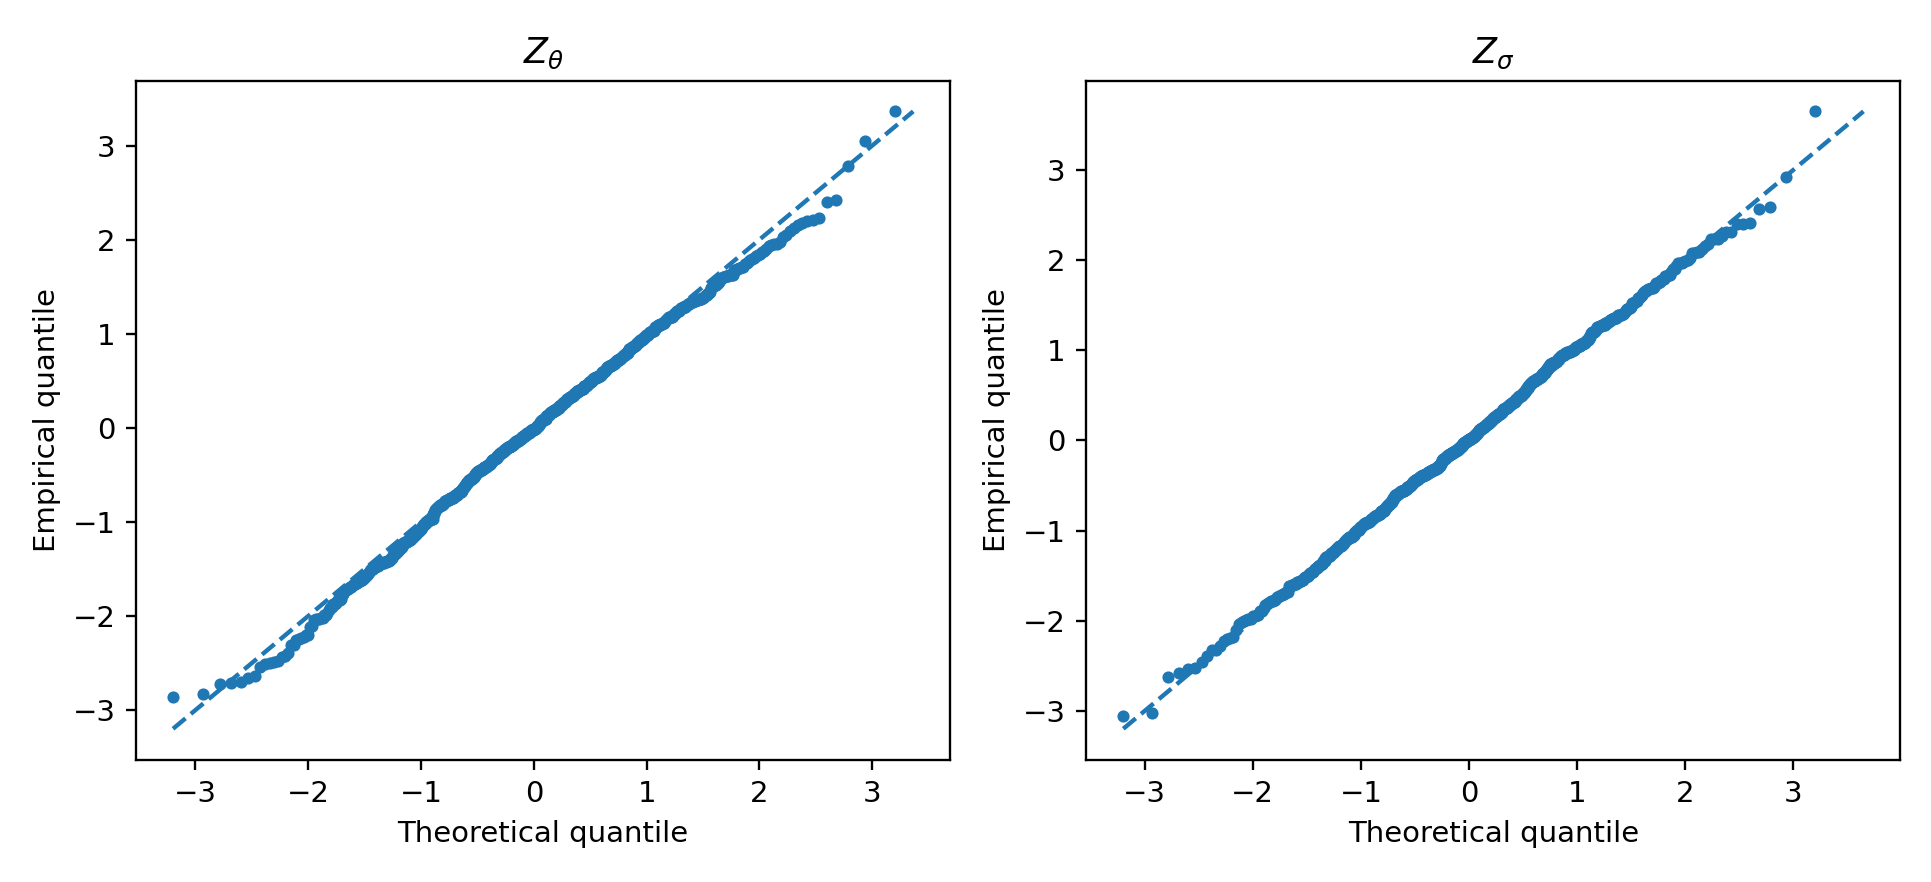
\includegraphics[width=.82\textwidth]{lan_qq_plots.png}
\caption{Normal quantile--quantile diagnostics for the standardised estimators. The visible right-skew of $Z_\theta$ at $N=5$ (skewness $0.49$, Kolmogorov--Smirnov $p=0.021$) dissipates along the design path ($p=0.42$ at $N=10$, $p=0.75$ at $N=20$), consistent with the first-order asymptotics.}
\label{fig:lan-qq}
\end{figure}

\subsection{Counterfactual process and bootstrap}

Fixed-intervention CDF sup-norm RMSE decreases from approximately $1.72\times10^{-3}$ to $2.13\times10^{-4}$. Distributional-effect sup-norm RMSE decreases from $1.64\times10^{-2}$ to $2.26\times10^{-3}$. Simultaneous coverage remains close to $0.95$ for both rate families.

\begin{table}[t]
\centering
\caption{Uniform target error and simultaneous coverage.}
\begin{tabular}{rrrrr}
\toprule
$N$ & CDF sup RMSE & Effect sup RMSE & Fast coverage & Slow coverage\\
\midrule
5  & $1.72\times10^{-3}$ & $1.64\times10^{-2}$ & 0.946 & 0.950\\
10 & $6.04\times10^{-4}$ & $6.29\times10^{-3}$ & 0.955 & 0.948\\
20 & $2.13\times10^{-4}$ & $2.26\times10^{-3}$ & 0.951 & 0.951\\
\bottomrule
\end{tabular}
\label{tab:coverage}
\end{table}

\begin{figure}[t]
\centering
\begin{subfigure}{.46\textwidth}
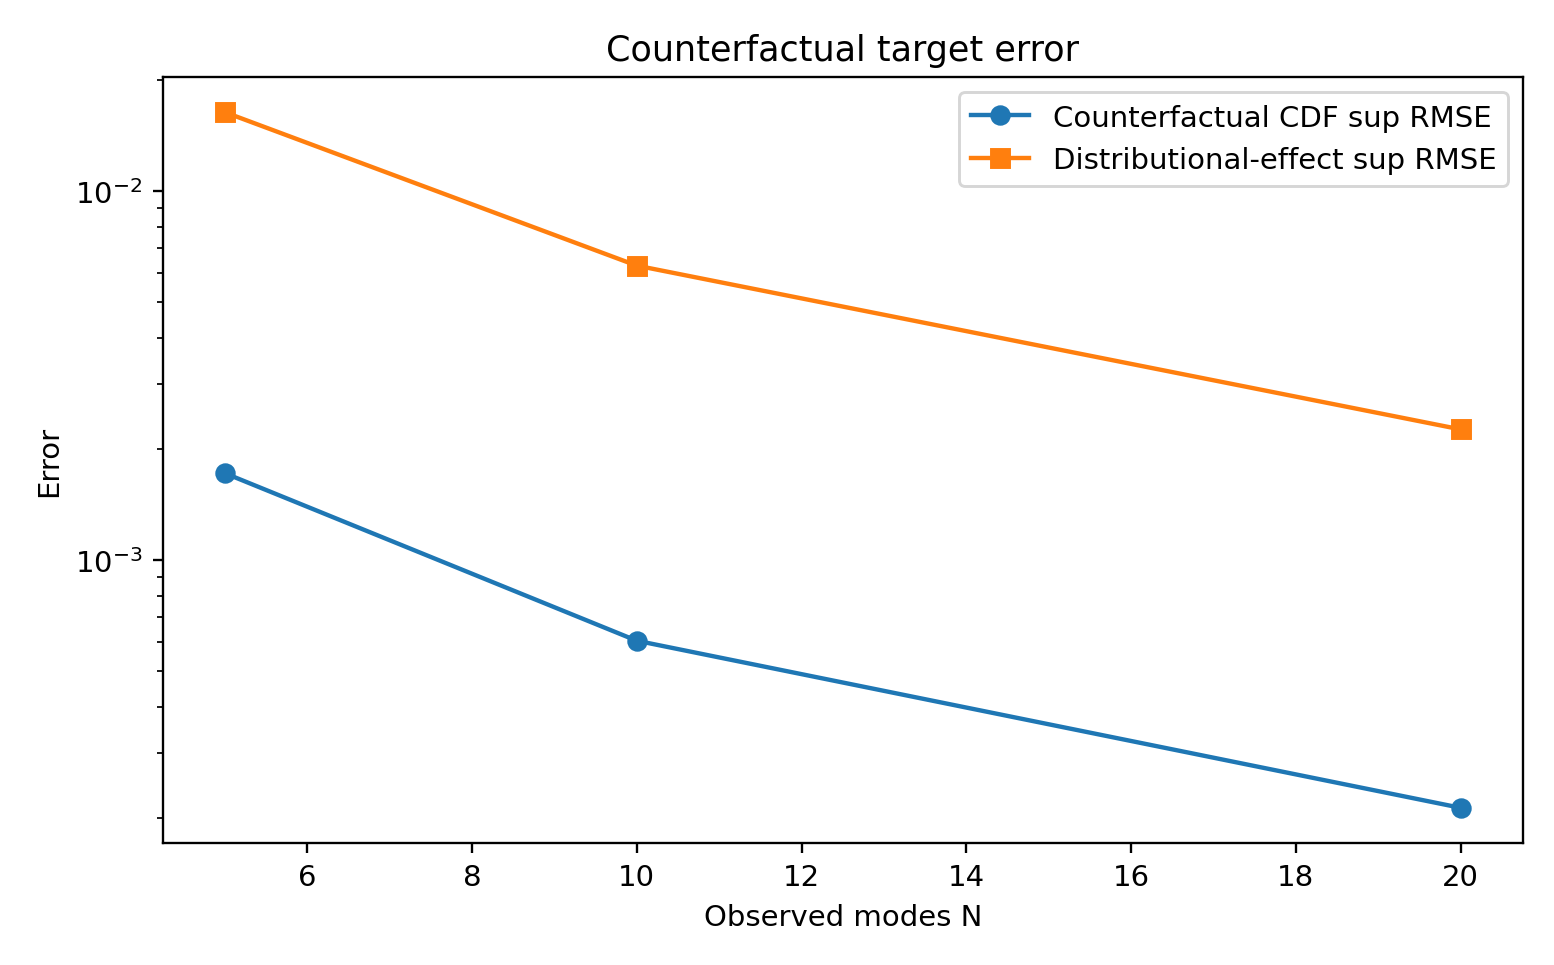
\includegraphics[width=\textwidth]{counterfactual_target_errors.png}
\caption{Uniform target errors.}
\end{subfigure}
\begin{subfigure}{.46\textwidth}
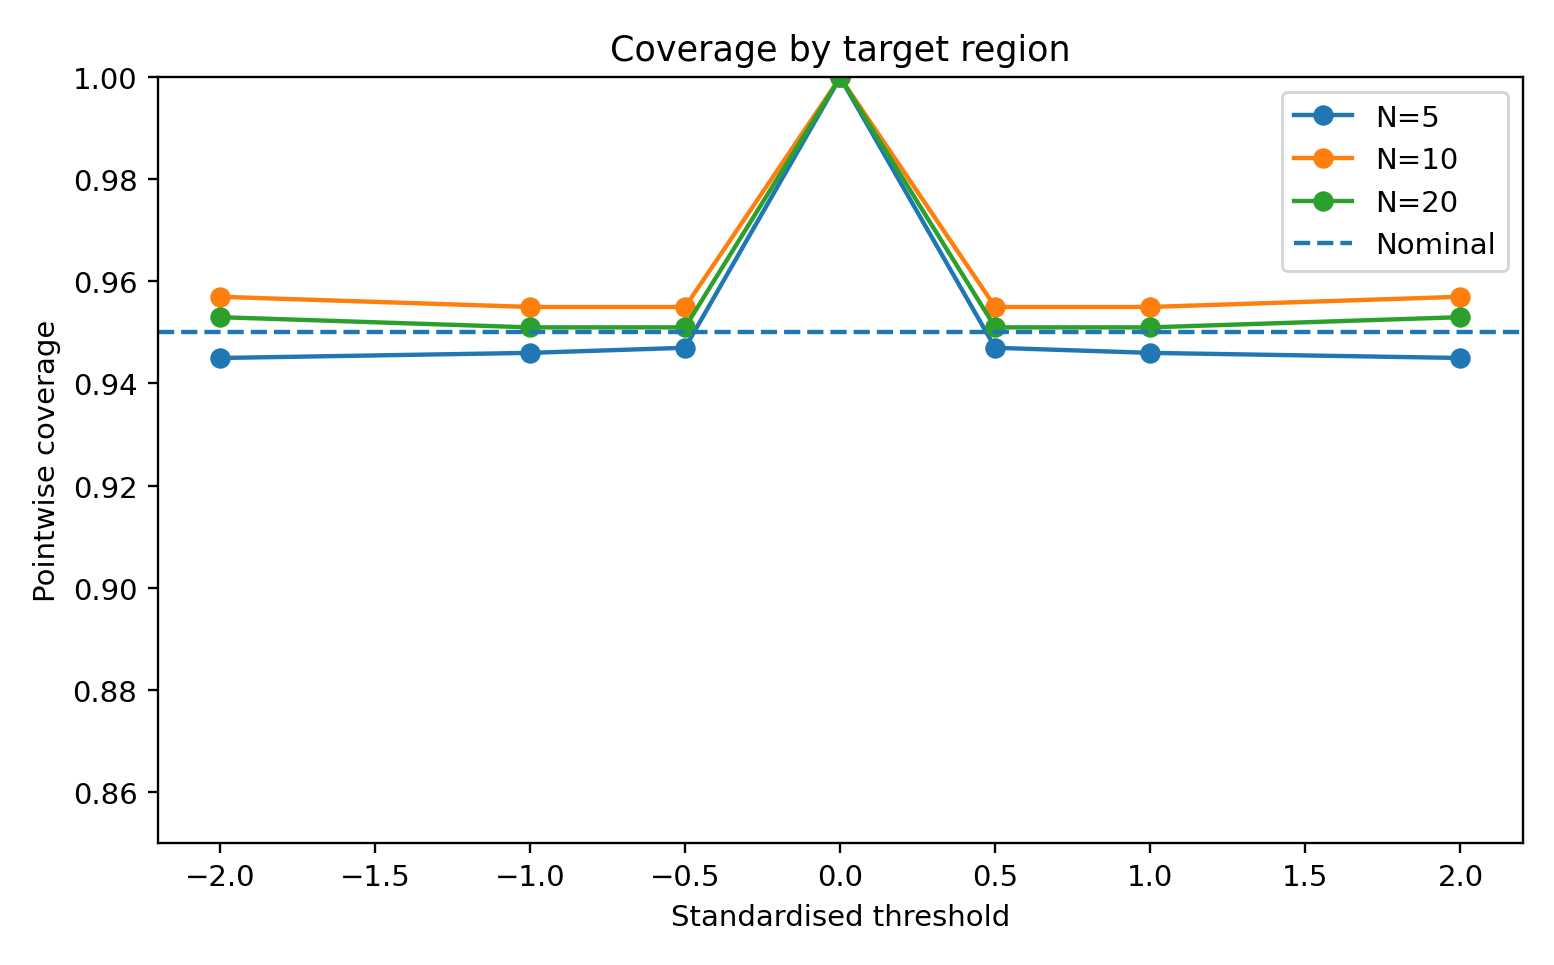
\includegraphics[width=\textwidth]{pointwise_coverage_by_threshold.png}
\caption{Coverage across thresholds.}
\end{subfigure}
\caption{Counterfactual target accuracy and coverage.}
\end{figure}

Beyond the headline coverage, the multiplier construction itself was stress-tested at $(N,n)=(10,8000)$ with $300$ replications per variant: the direct Gaussian draw, the modal-score multiplier with Gaussian weights, and the modal-score multiplier with Rademacher weights give statistically indistinguishable simultaneous coverage, and coverage is flat in the number of draws and in the threshold-grid resolution.

\begin{table}[t]
\centering
\caption{Bootstrap implementation sensitivity at $(N,n)=(10,8000)$, $300$ replications per row (Monte Carlo s.e.\ $\approx0.013$); nominal level $0.95$.}
\label{tab:boot-sens}
\begin{tabular}{llrrr}
\toprule
axis & variant & draws & fast cov. & slow cov.\\
\midrule
multiplier & direct Gaussian & 499 & 0.933 & 0.930\\
multiplier & modal Gaussian & 499 & 0.960 & 0.947\\
multiplier & modal Rademacher & 499 & 0.957 & 0.947\\
draws & direct Gaussian & 199 & 0.940 & 0.937\\
draws & direct Gaussian & 999 & 0.940 & 0.927\\
grid ($11$ pts) & direct Gaussian & 499 & 0.933 & 0.927\\
grid ($61$ pts) & direct Gaussian & 499 & 0.937 & 0.920\\
\bottomrule
\end{tabular}
\end{table}

\subsection{Approximation and sensitivity}

For the baseline spatial design, fitted log--log slopes are $-2.580$ for the mean tail, $-4.564$ for the variance tail, $-2.307$ for the strong RMS error, and $-2.580$ for the Gaussian CDF error, close to the theoretical values $-2.6,-4.6,-2.3,-2.6$. Temporal slopes lie between $0.994$ and $0.999$.

\begin{figure}[t]
\centering
\begin{subfigure}{.46\textwidth}
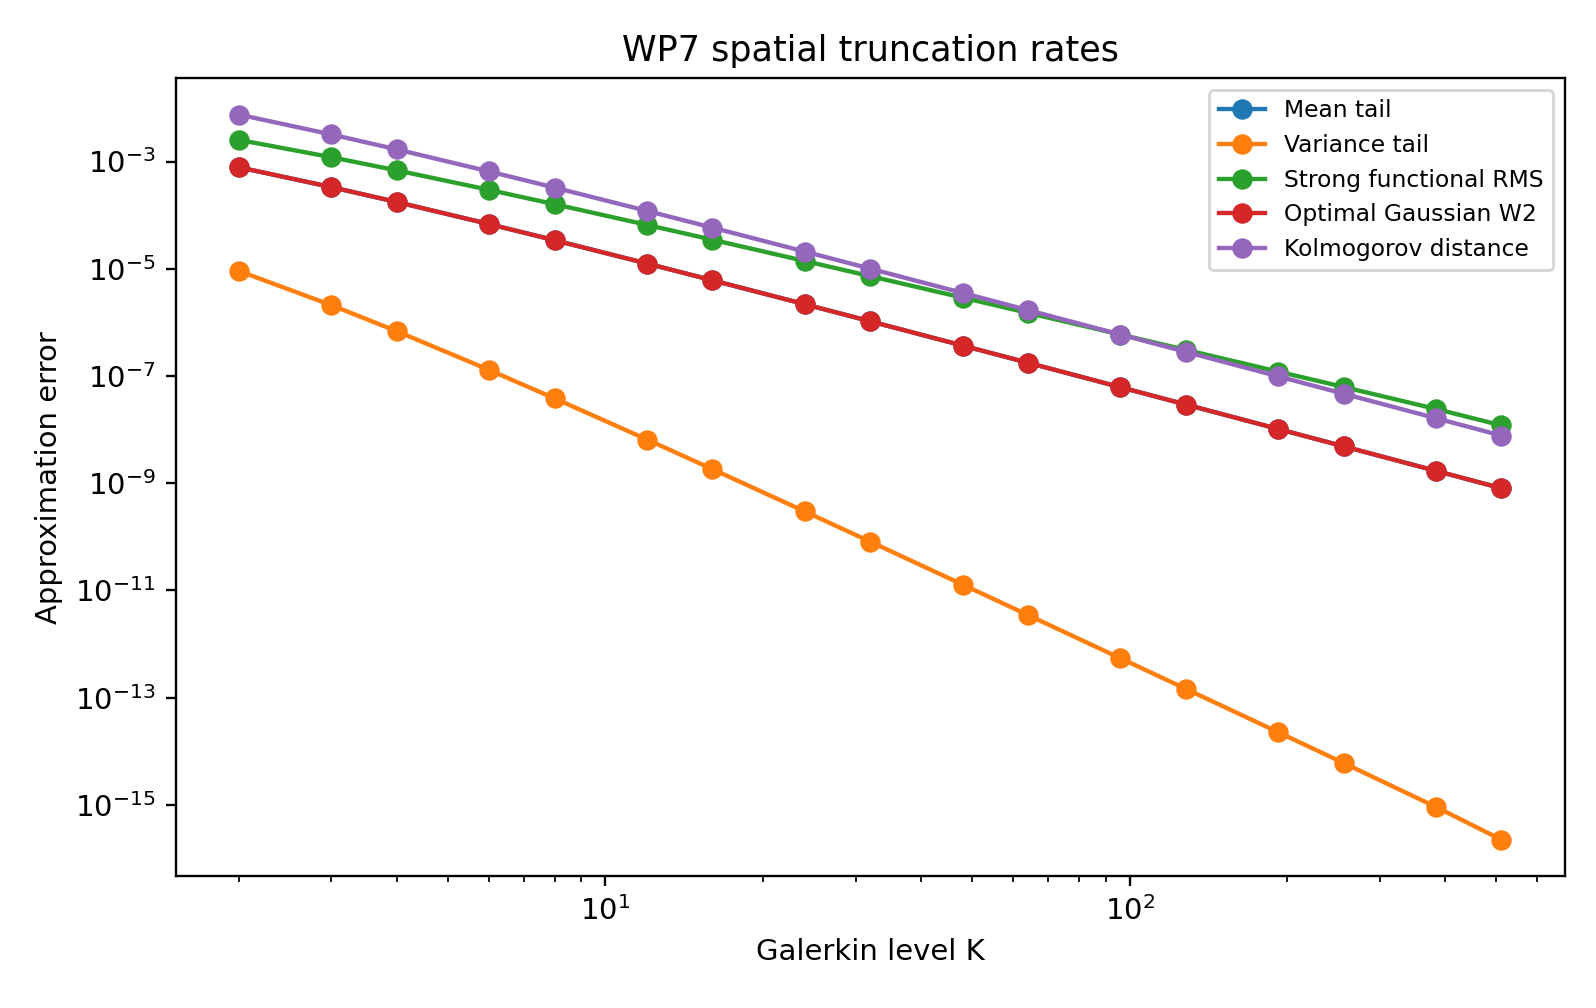
\includegraphics[width=\textwidth]{spatial_rates_baseline.png}
\caption{Galerkin rates.}
\end{subfigure}
\begin{subfigure}{.46\textwidth}
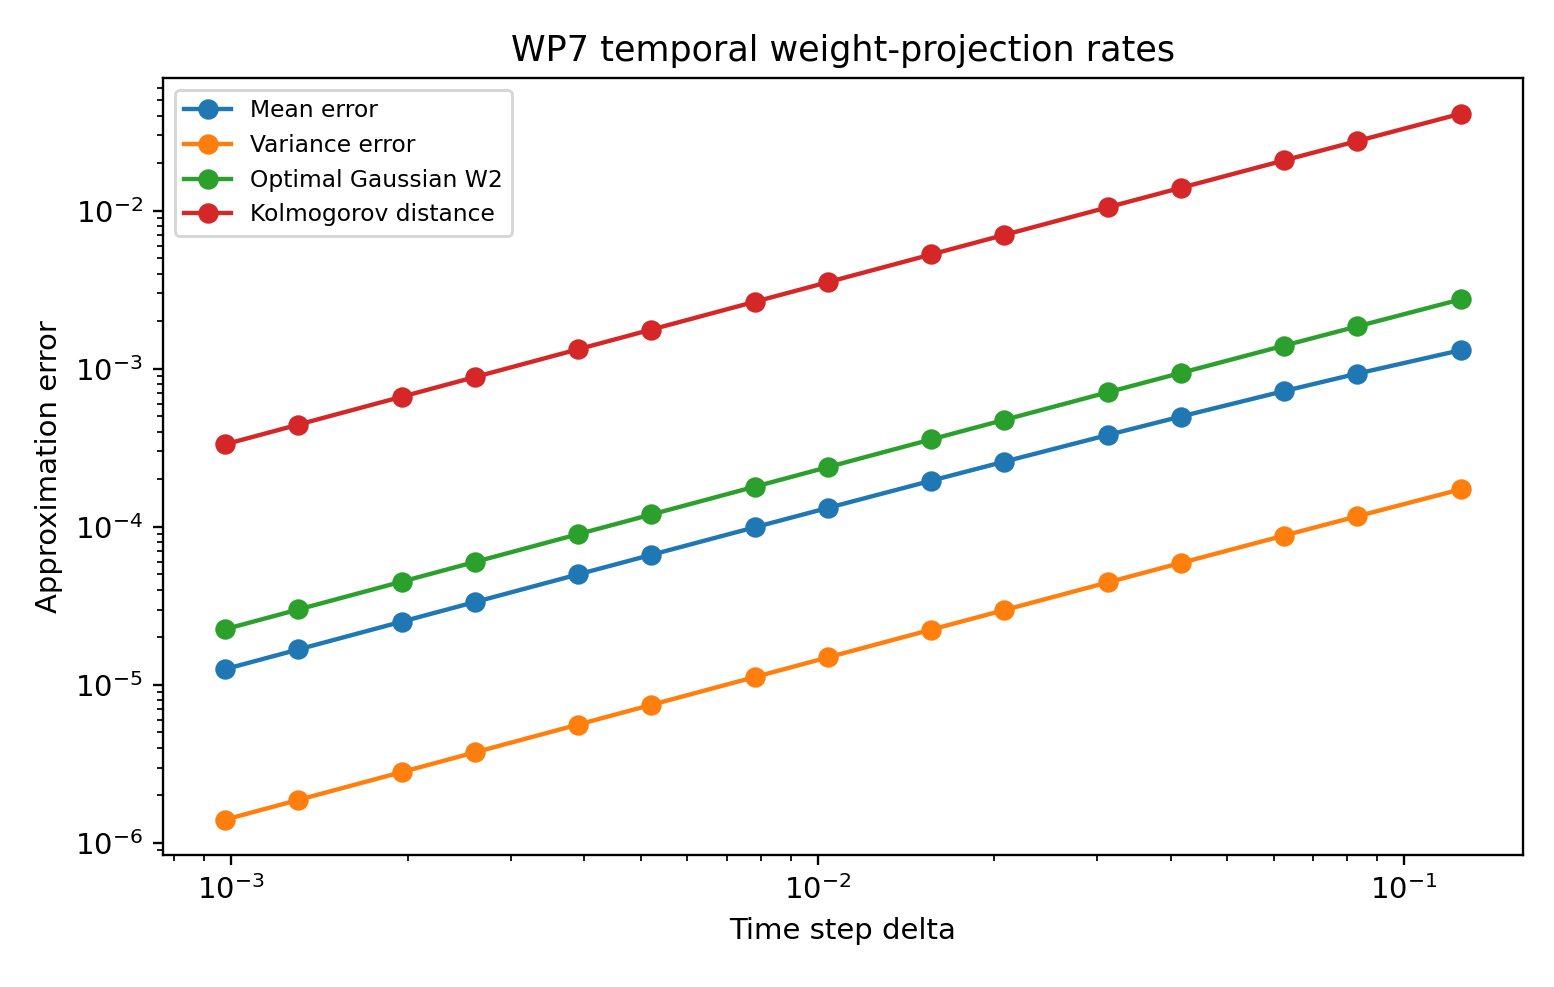
\includegraphics[width=\textwidth]{temporal_rates.png}
\caption{Temporal rates.}
\end{subfigure}
\caption{Deterministic approximation diagnostics.}
\end{figure}

For a non-commuting bounded perturbation, the central finite-difference derivative error decreases from $4.27\times10^{-6}$ at $\varepsilon=0.1$ to $1.71\times10^{-9}$ at $\varepsilon=0.002$. The CDF linearisation remainder is quadratic and the exact Gaussian $W_2$ distance remains below the derived Lipschitz envelope.

\subsection{Impossibility constructions}

The non-identification experiments are exact calculations rather than power studies. The adapted-feedback factual variance gap is zero while the post-intervention Kolmogorov distance is $0.0359$. The one-time open-loop factual variance gap is numerical zero and its post-intervention distance is $0.0984$. On a four-time grid, the factual covariance gap is $8.2\times10^{-16}$ while the post-intervention covariance gap is $0.7003$.


All tables and the headline diagnostics are regenerated by \texttt{make reproduce-publication}; the paper figures are regenerated end-to-end by the seeded validation pipeline (\texttt{make reproduce-paper}). The code records seeds, profiles, runtime, environment versions, and checksums.

\section{Discussion}

The paper places a narrow causal object on a complete mathematical and inferential footing. The intervention is an operator-module replacement inside a declared linear Gaussian SPDE class. The target is a counterfactual field-functional distribution. Identification is target specific. The inferential limit is mixed rate. Numerical approximation must be controlled at the target family's root-information scale.

Three distinctions are particularly important.

First, semantics and identification are separate. \Cref{sec:semantics} provides a coherent shared-noise intervention even before one asks whether the resulting law is recoverable from factual data; \Cref{sec:identification,sec:nonid} then characterise the positive and negative identification results.

Second, strong field approximation and Gaussian law approximation need not have the same rate. Under non-degeneracy, the variance tail enters normal CDF, quantile, and optimal Wasserstein comparisons linearly. Using the common-noise strong rate for every law target can be unnecessarily conservative.

Third, the phrase ``causal SPDE'' should not be read as unrestricted causal discovery. The intervention and invariant modules must be supplied. The feedback-gauge and open-loop constructions show that passive equality of factual laws cannot decide which part of a drift is the module that should be replaced.

Several extensions remain. Non-diagonal unbounded perturbations, including spatially varying divergence-form coefficients, require domain-sensitive perturbation theory. Semilinear equations require differentiability of nonlinear solution maps. Non-Gaussian noise calls for characteristic-function, Wasserstein, or quantile-specific methods rather than Gaussian mean--variance reduction. Physical-space observations require a separate statistical experiment and may produce different rates.

The present results are nevertheless sufficient for a coherent paper-level conclusion:
\begin{equation*}
\begin{aligned}
&\text{specified structural intervention}
+\text{identified factual experiment}\\
&\quad+\text{controlled numerical approximation}\\
&\hspace{2.5cm}\Longrightarrow
\text{uniformly inferable counterfactual laws}.
\end{aligned}
\end{equation*}
The impossibility results define the boundary of that conclusion rather than an exception to it.


\section*{Declarations}
\paragraph{Funding.} This work was supported by a DS4H (Digital Systems
for Humans) fellowship, Universit\'e C\^ote d'Azur.
\paragraph{Competing interests.} The author declares no competing interests.
\paragraph{Data and code availability.} All numerical results are generated
by the seeded replication package (Python reference implementation with a
Julia parity implementation, deterministic profiles, SHA-256 manifests, and
continuous-integration checks) archived with the manuscript sources; the
figures and tables of Section~\ref{sec:numerics} are reproduced end-to-end
by the documented \texttt{make} targets. [Repository DOI to be added upon
archival deposition.]
\paragraph{Acknowledgements.} Grammarly and generative AI tools were used
for proofreading, grammatical corrections, and targeted suggestions to
enhance sentence clarity. After using these tools, all authors reviewed and
edited the manuscript, taking full responsibility for its contents.

\bibliographystyle{plainnat}
\bibliography{references_merged}
\end{document}
"
% which silences the flags (status tracked in CHANGES_v2.md).
\ifdefined\SUBMISSIONCLEAN
\newcommand{\closuredraft}{}
\else
\newcommand{\closuredraft}{\par\smallskip\noindent
\textcolor{blue!55!black}{\footnotesize\textbf{[Verification
pending.]}}\par\smallskip}
\fi

\title{\textbf{Operator Interventions in Linear SPDEs:\\
Galerkin Structural Semantics, Mixed-Rate Local Asymptotic Normality,\\
and Uniform Inference for Post-Intervention Laws}}
\author{Gabriel Lucas St\'ephane Bontemps\thanks{Email:
\texttt{[address]}. ORCID: \texttt{[id]}.}\\[2pt]
{\normalsize GREDEG--CNRS, Universit\'e C\^ote d'Azur, Nice, France}\\
{\normalsize Adaptive Decision Lab, University of Oxford, Oxford, United Kingdom}}
\date{\ifdefined\SUBMISSIONCLEAN July 2026\else Working paper v4 (proto-submission draft), July 2026\fi}

\begin{document}
\maketitle

\begin{abstract}
We develop a causal-statistical theory for operator interventions in linear parabolic stochastic partial differential equations. The intervention replaces the generator coefficient while preserving the initial condition, noise spectrum, scale, observation mechanism, and primitive Wiener process. We first prove that the post-intervention SPDE is the infinite-dimensional limit of intervened Galerkin structural causal models driven by common exogenous Brownian segments. For Gaussian field functionals we give explicit post-intervention laws and necessary-and-sufficient target-identification criteria. Under exact discrete spectral observation, the likelihood is regular but anisotropic: the drift parameter is learned at rate $\sqrt{\sum_{k\le N}\lambda_k}$, whereas the noise scale is learned at rate $\sqrt{Nn}$. We establish local asymptotic normality, efficient estimation, uniform counterfactual CDF, quantile, tail, and distributional-effect processes, and feasible simultaneous confidence bands based on modal-score multipliers. We derive Fr\'echet derivatives of the operator-to-law map, combine statistical, Galerkin, temporal, and bounded operator-approximation errors, and state rate conditions for full-field inference. Finally, we construct observationally equivalent mechanisms with different post-intervention laws when forcing, initial, sensing, or cross-world modules are left unrestricted. Complete proofs are contained in the paper; numerical experiments verify the mixed rates, simultaneous coverage, approximation slopes, operator sensitivities, and impossibility constructions.
\end{abstract}

\noindent\textbf{Keywords:} stochastic partial differential equations; operator intervention; spectral inference; local asymptotic normality; empirical processes; multiplier bootstrap; Galerkin approximation.\\
\textbf{MSC2020:} 60H15; 62M05; 62F12; 62G15; 65M60.

% ---------- statements ----------
\section{Introduction}

Many scientific interventions change a law of motion rather than a scalar treatment. Diffusivity can be altered by a material, a boundary protocol can change a transport operator, and a spatial policy can modify the generator of a stochastic field. In these settings the object of interest is not merely a parameter. It is a post-intervention distribution of a functional of the field.

We study the linear parabolic model
\begin{equation}\label{eq:intro-spde}
 dU_t=\theta A_0U_t\,dt+\sigma Q^{1/2}dW_t,
 \qquad U_0=u_0,
\end{equation}
where $A_0$ is self-adjoint, negative, and has compact resolvent. The primary intervention is
\[
 \doop(\theta=\widetilde\theta),
\]
which replaces $\theta A_0$ by $\widetilde\theta A_0$ while leaving the other structural modules invariant. For a space-time weight $w$, the target is
\begin{equation}\label{eq:intro-target}
 F_{\widetilde\theta,w}(z;\vartheta)
 =\Pp_{\vartheta}\left\{
 \int_0^T\inner{w_t}{U_t^{\widetilde\theta}}\,dt\le z
 \right\},
 \qquad \vartheta=(\theta,\sigma).
\end{equation}

The paper addresses four distinct questions. First, what makes the formal replacement of an operator a structural intervention rather than a relabelled stochastic equation? Second, when is the counterfactual law identified from a factual observation experiment? Third, how can it be estimated uniformly over interventions, weights, and thresholds? Fourth, how do statistical and numerical errors interact at the inferential scale?

Our construction extends the finite-dimensional intervention logic of \citet{SokolHansen2014} to a diagonal parabolic SPDE. The post-intervention field is represented as the limit of intervened Galerkin structural causal models using the same Brownian path segments in every world. This common-noise convention is stronger than specifying marginal laws; it fixes the primitive disturbances that remain invariant under the intervention.

The statistical experiment uses exact discrete observations of the first $N$ spectral coordinates. This setting is close to the spectral inference literature surveyed by \citet{Cialenco2018}, but the target and asymptotic geometry are different. The exact transition likelihood produces two rates. With $\Lambda_N=\sum_{k\le N}\lambda_k$,
\[
 \sqrt{\Lambda_N}(\widehat\theta-\theta_0)
 \quad\text{and}\quad
 \sqrt{Nn}(\widehat\sigma-\sigma_0)
\]
have non-degenerate limits. Fixed absolute-intervention laws overwrite the factual drift and are therefore estimated at the faster scale rate. Factual and factual-versus-counterfactual effects retain the slower drift uncertainty.

The main contributions are as follows.

\begin{enumerate}[label=(\roman*)]
\item We prove exact finite-dimensional intervention semantics and uniform convergence of intervened Galerkin models to the post-intervention SPDE.
\item We give a fibre criterion for target identification and explicit finite-sample identification results under exact and noisy spectral observations.
\item We derive the exact likelihood, mixed Fisher-information limit, LAN expansion, efficient MLE, and moment convergence.
\item We establish uniform plug-in processes in $C(\cT)$, feasible multiplier bands, and contact-set tests for one-sided counterfactual hypotheses.
\item We prove operator-to-law derivatives for bounded perturbations and a separate analytic-semigroup theorem for the unbounded rescaling direction $A_0$.
\item We combine statistical, Galerkin, temporal, and operator approximation errors in one family-specific inference theorem.
\item We construct sharp non-identification examples. In particular, unrestricted feedback or open-loop forcing can absorb the factual operator and separate only after intervention.
\end{enumerate}

The contribution is deliberately narrower than causal discovery. The intervention is specified by the analyst. The theory identifies its target inside an admissible model class. It does not infer a causal graph from passive field observations, and it does not claim that every decomposition of an observed drift is structural.

\subsection*{Related literature}

Three literatures meet in this paper, and the delimitation matters.

\paragraph{Statistics for SPDEs.}
The spectral approach to drift estimation under continuous observation goes
back to \citet{HuebnerRozovskii1995}; see \citet{Lototsky2009} and the survey
of \citet{Cialenco2018}. An active recent strand studies discretely observed
parabolic equations: power variations and volatility estimation under
high-frequency sampling \citep{BibingerTrabs2020,Chong2020}, joint estimation
from space--time grids
\citep{HildebrandtTrabs2021,KainoUchida2021,TonakiKainoUchida2023,TonakiKainoUchida2024},
drift estimation from discretely sampled Fourier modes
\citep{CialencoDelgadoVencesKim2020}, local measurements
\citep{AltmeyerReiss2021}, and semilinear extensions
\citep{PasemannStannat2020}. Relative to this literature our observation
scheme is deliberately the cleanest one --- exact discrete observation of $N$
spectral coordinates --- but the output is of a different kind: a
\emph{joint} local asymptotic normality expansion with anisotropic diagonal
normalisation $\diag(\sqrt{\Lambda_N},\sqrt{Nn})$, efficiency and moment
convergence of the exact conditional MLE, pushed through to uniform
inference on post-intervention laws of field functionals. To our knowledge
both the mixed-rate LAN statement and any inferential theory for operator
interventions in SPDEs are new; the nearest discrete-observation results
concern estimation rates rather than experiment-level asymptotics.

\paragraph{Causal models for dynamical systems.}
Interventions in ODE systems were formalised as limits of structural
equation models by \citet{MooijJanzingScholkopf2013}, and extended to dynamic
equilibria and random differential equations by \citet{RubensteinEtAl2018}
and \citet{BongersMooij2018}; \citet{SokolHansen2014} treat SDEs via Euler
schemes, and \citet{PetersBauerPfister2022} survey the programme.
\Cref{thm:semantics} is the infinite-dimensional counterpart: the
post-intervention SPDE is the limit of intervened Galerkin structural causal
models driven by \emph{common} Brownian segments, so the intervention is
module surgery in the sense of \citet{Haavelmo1944} rather than a
relabelling of stochastic equations. The non-identification constructions of
\Cref{sec:nonid} calibrate exactly which invariances carry identifying
content.

\paragraph{Uniform inference on distributional targets.}
The plug-in processes and feasible bands use the functional delta method
\citep{vanDerVaart1998,vanDerVaartWellner1996}, multiplier approximations
for suprema \citep{ChernozhukovChetverikovKato2013}, directional
differentiability \citep{FangSantos2019}, and contact-set logic
\citep{AndrewsSoares2010,LintonSongWhang2010}. The finite-rank limit
geometry --- every target process is a deterministic derivative surface
loading a two-dimensional Gaussian --- makes these tools exact rather than
high-dimensional approximations, and the mixed rates propagate to
target-specific band widths. In econometric terms the targets are
counterfactual distributions and quantiles
\citep{ChernozhukovFernandezValMelly2013}; identification from discretely
sampled continuous-time dynamics connects to the aliasing literature
(\Cref{rem:no-aliasing}).

The paper is organised as follows. \Cref{sec:model} states the model and Gaussian target law. \Cref{sec:semantics} proves the intervention semantics. \Cref{sec:identification} treats identification. \Cref{sec:lan} develops the statistical experiment. \Cref{sec:uniform} gives uniform inference and bootstrap procedures. \Cref{sec:sensitivity} treats operator response and total error. \Cref{sec:nonid} gives the impossibility boundary. \Cref{sec:numerics} reports numerical validation. \ifdefined\MERGEDDOC Complete proofs of every statement are collected in \Cref{sec:proofs} (parts S0--S8), in dependency order and preceded by part S0, which restates every imported external theorem as an attributed local proposition whose hypotheses are verified at each point of use.\else Complete proofs of every statement are collected in the accompanying consolidated technical supplement (parts S0--S8), which supersedes the separate work-package archives; part S0 restates every imported external theorem as an attributed local proposition whose hypotheses are verified at each point of use.\fi

\subsection*{Notation}
$H=L^2(D)$ with inner product $\inner\cdot\cdot$ and norm $\norm\cdot$; $A_0$ is self-adjoint, negative, with compact resolvent, eigenpairs $(-\lambda_k,e_k)$, $0<\lambda_1\le\lambda_2\le\cdots$, and $\lambda_k\asymp k^{2/d}$ (Weyl growth). $\Lambda_N:=\sum_{k\le N}\lambda_k$. The parameter is $\vartheta=(\theta,\sigma)$, its true value $\vartheta_0$, and $A_{N,n}:=\diag(\sqrt{\Lambda_N},\sqrt{Nn})$ is the information normalisation. $\doop(\theta=\tilde a)$ denotes module surgery on the generator coefficient. Weak convergence is $\Rightarrow$; $\op(1),\Op(1)$ are stochastic order symbols; $C,c$ denote finite positive constants that may change between displays and whose dependencies are stated where they matter; $a\wedge b=\min(a,b)$, $a\vee b=\max(a,b)$, and $x_+=\max(x,0)$. For a compact index set $\cT$, $C(\cT)$ carries the supremum norm $\norm\cdot_\infty$. \ifdefined\MERGEDDOC\else \Cref{tab:crosswalk} maps each statement to its proof.\fi

\ifdefined\MERGEDDOC\else
\begin{table}[t]
\centering\small
\caption{Statement-to-proof crosswalk\ifdefined\MERGEDDOC\ (\Cref{sec:proofs})\else\ (technical supplement)\fi.}
\label{tab:crosswalk}
\begin{tabular}{ll}
\toprule
Main-text statement & Proof location \\
\midrule
\Cref{prop:gaussian-law} & Part S2 (Gaussian post-intervention law)\\
\Cref{prop:exact-scm,thm:semantics} & Part S1 (exact representation; Galerkin limits)\\
\Cref{thm:fibre,thm:exact-id,prop:partial} & Part S2 (identification)\\
\Cref{thm:lan} & Part S3 (LAN, efficiency, moment convergence)\\
\Cref{thm:processes,thm:quantile-tail} & Part S4 (uniform target processes)\\
\Cref{thm:bands} & Part S5 (multiplier, floor bands, contact sets)\\
\Cref{thm:sensitivity} & Part S6 (operator sensitivity)\\
\Cref{thm:total-error} & Part S7 (total error)\\
\Cref{thm:gauge-main,thm:nonid-assembly} & Part S8 (non-identification)\\
\bottomrule
\end{tabular}
\end{table}
\fi

\section{Model and counterfactual targets}\label{sec:model}

Let $D\subset\R^d$ be bounded and regular, and let $H=L^2(D)$. Let $A_0:D(A_0)\subset H\to H$ be densely defined, self-adjoint, negative, and have compact resolvent. There is an orthonormal basis $(e_k)_{k\ge1}$ and eigenvalues $0<\lambda_1\le\lambda_2\le\cdots$ such that
\[
 A_0e_k=-\lambda_ke_k,
 \qquad
 \lambda_k\asymp k^{2/d}.
\]
Let $W_t=\sum_{k\ge1}\beta_k(t)e_k$ be cylindrical Wiener noise and let $Q^{1/2}e_k=q_ke_k$.

\begin{assumption}[Positive core]\label{ass:core}
The factual parameter belongs to a compact rectangle
\[
 \vartheta=(\theta,\sigma)\in
 [\underline\theta,\overline\theta]\times
 [\underline\sigma,\overline\sigma]\Subset(0,\infty)^2.
\]
The intervention set $\widetilde\Theta$ is a compact subset of $(0,\infty)$. The initial state is deterministic. At minimum,
\[
 \sum_{k\ge1}\frac{q_k^2}{\lambda_k}<\infty.
\]
For pathwise Galerkin rates we impose the stronger fractional summability stated in \Cref{sec:semantics}.
\end{assumption}

The factual mild solution is
\[
 U_t^\theta
 =e^{t\theta A_0}u_0
 +\sigma\int_0^t e^{(t-s)\theta A_0}Q^{1/2}dW_s.
\]
The intervention replaces only the generator coefficient:
\begin{equation}\label{eq:cf-spde}
 dU_t^{a}=aA_0U_t^{a}\,dt+\sigma Q^{1/2}dW_t,
 \qquad U_0^a=u_0,
 \qquad a\in\widetilde\Theta.
\end{equation}
All fields in \eqref{eq:cf-spde} are constructed with the same $u_0,Q,\sigma$, and $W$.

For $w\in L^2(0,T;H)$ define
\[
 \Psi_w(U)=\int_0^T\inner{w_t}{U_t}\,dt.
\]
Write $w_k(t)=\inner{w_t}{e_k}$ and $u_{0,k}=\inner{u_0}{e_k}$. The law of $\Psi_w(U^a)$ is obtained in three displayed steps. Modally, $u^a_k(t)=e^{-a\lambda_kt}u_{0,k}+\sigma q_k\int_0^te^{-a\lambda_k(t-s)}d\beta_k(s)$, so
\[
 \Psi_w(U^a)
 =\sum_{k\ge1}\int_0^Tw_k(t)u^a_k(t)\,dt
 =m_a(w)+\sigma\sum_{k\ge1}q_k\int_0^T\!\!w_k(t)\!\int_0^t
 e^{-a\lambda_k(t-s)}\,d\beta_k(s)\,dt .
\]
The stochastic Fubini interchange (Part S0, imported stochastic Fubini theorem) applies because
\[
 \int_0^T\Big(\E\int_0^T w_k(t)^2e^{-2a\lambda_k(t-s)}\mathbf 1_{s\le t}\,dt\Big)^{1/2}ds
 \le\sqrt T\,\norm{w_k}_{L^2}<\infty
 \qquad\text{for each }k,
\]
and exchanging the two integrals collects, for each innovation time $s$, the total future weight it loads:
\[
 \int_0^T\!\!w_k(t)\!\int_0^te^{-a\lambda_k(t-s)}d\beta_k(s)\,dt
 =\int_0^T\Big(\underbrace{\int_s^Tw_k(t)e^{-a\lambda_k(t-s)}\,dt}_{=\,g_{a,k,w}(s)}\Big)d\beta_k(s).
\]
Hence
\[
 \Psi_w(U^a)
 =m_a(w)+\sigma\sum_{k\ge1}q_k
 \int_0^T g_{a,k,w}(s)\,d\beta_k(s),
\]
where
\begin{align}
 m_a(w)
 &=\sum_{k\ge1}u_{0,k}\int_0^T w_k(t)e^{-a\lambda_kt}\,dt,\label{eq:mean}\\
 g_{a,k,w}(s)
 &=\int_s^T w_k(t)e^{-a\lambda_k(t-s)}\,dt.\label{eq:transfer}
\end{align}

\begin{proposition}[Gaussian counterfactual law]\label{prop:gaussian-law}
Under \Cref{ass:core},
\[
 \Psi_w(U^a)\sim N\bigl(m_a(w),\sigma^2V_a(w)\bigr),
\]
where
\begin{equation}\label{eq:variance}
 V_a(w)=\sum_{k\ge1}q_k^2\int_0^T g_{a,k,w}(s)^2\,ds.
\end{equation}
Consequently,
\[
 F_{a,w}(z;\sigma)
 =\Phi\left(
 \frac{z-m_a(w)}{\sigma\sqrt{V_a(w)}}
 \right).
\]
\end{proposition}

\inwords{The intervention law is explicit once the invariant structural modules are fixed. The factual drift parameter $\theta$ is absent from the fixed absolute-intervention law because it has been overwritten.}

The indexed target set is
\[
 \cT=\widetilde\Theta\times\cW\times\cZ,
\]
where $\cZ$ is compact and $\cW$ is a compact ellipsoid in a space-time Sobolev basis. For CDF and quantile inference we impose
\[
 \inf_{(a,w)\in\widetilde\Theta\times\cW}V_a(w)>0.
\]
Wasserstein and field-functional convergence do not require this non-degeneracy condition.

\begin{figure}[t]
\centering
\resizebox{.96\textwidth}{!}{% Modal decay under intervention and the transfer kernel g_{a,k,w}.
% Left: e^{-a lambda_k t} for factual theta vs intervened a on two modes.
% Right: the backward transfer kernel s -> g_{a,k,w}(s) for w_k = 1.
\begin{tikzpicture}[font=\small, scale=1.0,
  ax/.style={-{Stealth[length=2.2mm]}, thick},
  lbl/.style={font=\footnotesize\itshape, text=black!70}]
% ---------------- left panel: modal decay ----------------
\begin{scope}
\draw[ax] (0,0) -- (4.4,0) node[below left=1pt]{$t$};
\draw[ax] (0,0) -- (0,3.1);
\node[anchor=south, rotate=90] at (-.55,1.4) {$e^{-a\lambda_k t}$};
\draw (0.03,2.6) node[left, font=\scriptsize]{$1$} -- (-0.07,2.6);
% mode k=1: lambda=1 scaled; factual theta=0.7 -> rate .7; intervened a=1.4
\draw[thick, blue!60!black]  plot[domain=0:4, samples=60] (\x,{2.6*exp(-0.55*\x)});
\draw[thick, red!60!black, dashed] plot[domain=0:4, samples=60] (\x,{2.6*exp(-1.1*\x)});
% mode k=2: lambda 4x
\draw[thin, blue!60!black]  plot[domain=0:4, samples=60] (\x,{2.6*exp(-2.2*\x)});
\draw[thin, red!60!black, dashed] plot[domain=0:4, samples=60] (\x,{2.6*exp(-4.4*\x)});
\node[lbl, blue!60!black]  at (3.05,1.15) {factual $\theta$};
\node[lbl, red!60!black]   at (2.95,0.33) {intervened $\tilde a=2\theta$};
\node[lbl] at (2.2,-0.42) {mode $k=1$ (thick), $k=2$ (thin): $\lambda_2=4\lambda_1$};
\end{scope}
% ---------------- right panel: transfer kernel ----------------
\begin{scope}[xshift=7.1cm]
\draw[ax] (0,0) -- (4.4,0) node[below left=1pt]{$s$};
\draw[ax] (0,0) -- (0,3.1);
\node[anchor=south, rotate=90] at (-.55,1.4) {$g_{a,k,w}(s)$};
\draw (4.0,0.05) -- (4.0,-0.05) node[below, font=\scriptsize]{$T$};
% g(s) = (1 - e^{-a lambda (T-s)})/(a lambda) for w=1; a*lambda = .55 resp 1.1 (k=1)
\draw[thick, blue!60!black] plot[domain=0:4, samples=60]
  (\x,{2.6*(1-exp(-0.55*(4-\x)))/(0.55*4)*2.2});
\draw[thick, red!60!black, dashed] plot[domain=0:4, samples=60]
  (\x,{2.6*(1-exp(-1.1*(4-\x)))/(1.1*4)*2.2});
\node[lbl, align=left, anchor=west] at (1.45,2.85)
  {$g_{a,k,w}(s)=\int_s^T w_k(t)e^{-a\lambda_k(t-s)}\,dt$\\[1pt]
   here $w_k\equiv1$: $g=\frac{1-e^{-a\lambda_k(T-s)}}{a\lambda_k}$};
\node[lbl, blue!60!black] at (1.15,1.28) {$a=\theta$};
\node[lbl, red!60!black]  at (1.28,0.44) {$a=\tilde a$};
\node[lbl, align=center] at (2.2,-0.42)
  {$V_a(w)=\sum_kq_k^2\!\int_0^T\!g_{a,k,w}^2$: intervention lowers the\\
   load of every innovation, monotonically in $a$};
\end{scope}
\end{tikzpicture}
}
\caption{The two ingredients of the post-intervention law. Left: modal decay $e^{-a\lambda_kt}$ under the factual coefficient and under $\doop(\theta=\tilde a)$, for a slow and a fast mode. Right: the backward transfer kernel $g_{a,k,w}$ collecting, for each innovation time $s$, the future weight it loads; by It\^o isometry the target variance is $\sigma^2\sum_kq_k^2\norm{g_{a,k,w}}_{L^2}^2$.}
\label{fig:transfer}
\end{figure}

\section{Galerkin structural intervention semantics}\label{sec:semantics}

Let $H_K=\operatorname{span}\{e_1,\ldots,e_K\}$ and let $P_K$ be the orthogonal projection. Fix a partition $0=t_0<\cdots<t_J=T$. For mode $k$ and interval $j$, use the Brownian segment
\[
 E_{k,j}(r)=\beta_k(t_j+r)-\beta_k(t_j),
 \qquad 0\le r\le\Delta_j,
\]
as the primitive exogenous variable.

For $a>0$, define the exact local map
\[
 G_{a,k,r}(x,e)
 =e^{-a\lambda_kr}x
 +\sigma q_k\mathfrak I_{a\lambda_k,r}(e),
\]
where
\begin{equation}\label{eq:pathmap}
 \mathfrak I_{c,r}(e)
 =e(r)-c\int_0^r e^{-c(r-s)}e(s)\,ds.
\end{equation}
The map in \eqref{eq:pathmap} is continuous on $C_0([0,r])$. For Brownian $e$ it equals the It\^o convolution
\[
 \int_0^r e^{-c(r-s)}de(s)
\]
by integration by parts. Thus the structural equation is a measurable, indeed continuous, function of the primitive Brownian segment.

The finite model recursively applies $G_{a,k,r}$ to every mode and interval. The intervention $\doop(\theta=a)$ replaces the family $G_{\theta,k,r}$ by $G_{a,k,r}$ while preserving all exogenous segments.

\begin{proposition}[Exact structural representation]\label{prop:exact-scm}
For every $K$, partition, and $a\in\widetilde\Theta$, the intervened structural recursion equals the exact projected post-intervention SPDE path:
\[
 \mathcal X_t^{K,\doop(\theta=a)}
 =U_t^{K,a}
 =P_KU_t^a
 \quad\text{for all }t\in[0,T]
 \quad\text{almost surely}.
\]
\end{proposition}

\begin{theorem}[Galerkin limits of intervened SCMs]\label{thm:semantics}
Assume, for some $\alpha\ge0$ and $\delta>0$,
\[
 u_0\in D((-A_0)^\alpha),
 \qquad
 \sum_{k\ge1}q_k^2\lambda_k^{2(\alpha+\delta)-1}<\infty.
\]
Then
\[
 \sup_{a\in\widetilde\Theta}
 \E\sup_{t\le T}
 \norm{U_t^a-P_KU_t^a}_H^2
 \le C\lambda_{K+1}^{-2\alpha}.
\]
Under only $u_0\in H$ and $\sum q_k^2/\lambda_k<\infty$,
\[
 \sup_a\E\int_0^T\norm{U_t^a-P_KU_t^a}^2dt\to0.
\]
Finally, for every bounded $\cW\subset L^2(0,T;H)$,
\[
 \sup_{a,w}
 \E\abs{\Psi_w(U^a)-\Psi_w(P_KU^a)}^2\to0,
\]
and the corresponding laws converge uniformly in quadratic Wasserstein distance.
\end{theorem}

\inwords{The post-intervention SPDE is not introduced by notation alone. It is the limit of finite structural models whose operator mechanism is surgically replaced while the primitive shocks are fixed. \Cref{fig:modules} displays the two-world construction.}

\begin{figure}[t]
\centering
\resizebox{.98\textwidth}{!}{% Two-world common-noise construction. Design rules: one box per concept,
% at most one short label per arrow, labels never over lines or boxes.
\begin{tikzpicture}[
  font=\small,
  box/.style={draw, rounded corners=2pt, minimum width=3.4cm,
              minimum height=1.05cm, align=center},
  shared/.style={box, fill=gray!16, minimum width=3.9cm, minimum height=1.7cm},
  mechF/.style={box, fill=blue!10},
  mechI/.style={box, fill=red!9},
  law/.style={box, fill=green!11},
  flow/.style={-{Stealth[length=2.6mm]}, semithick},
  surg/.style={-{Stealth[length=3mm]}, very thick, red!70!black},
  lbl/.style={font=\footnotesize\itshape, text=black!70}
]
% shared primitives: one box
\node[shared] (prim) at (0,-2.2)
  {invariant modules\\[2pt]
   $W,\quad u_0,\quad Q^{1/2},\quad \sigma,\quad \mathcal H$};

% factual row (y=0)
\node[mechF] (Gf) at (5.4,0)  {mechanism\\[-1pt] $dU=\theta A_0U\,dt+\sigma Q^{1/2}dW$};
\node[box]   (Uf) at (10.4,0) {field $U^{\theta}$};
\node[law]   (Yf) at (14.6,0) {observed law\\[-1pt] $Y_{k,j}=u_k(t_j)$};

% intervened row (y=-4.4)
\node[mechI] (Gi) at (5.4,-4.4)  {mechanism\\[-1pt] $dU=\tilde aA_0U\,dt+\sigma Q^{1/2}dW$};
\node[box]   (Ui) at (10.4,-4.4) {field $U^{\tilde a}$};
\node[law]   (Ti) at (14.6,-4.4) {target law\\[-1pt] $F_{\tilde a,w}$};

% shared -> mechanisms (two clean diagonals from box corners)
\draw[flow] (prim.north east) -- (Gf.west);
\draw[flow] (prim.south east) -- (Gi.west);
\node[lbl, anchor=north] at (2.15,-4.45) {same Brownian segments};

% rows
\draw[flow] (Gf) -- (Uf);
\draw[flow] (Uf) -- (Yf);
\draw[flow] (Gi) -- (Ui);
\draw[flow] (Ui) -- (Ti);
\node[lbl] at (12.5,0.72)  {spectral sampling};
\node[lbl] at (12.5,-3.68) {functional $\Psi_w$};

% surgery arrow, label fully to its left in white space
\draw[surg] (Gf.south) -- (Gi.north);
\node[font=\footnotesize, red!70!black, align=right, anchor=east] at (4.55,-2.2)
  {$\doop(\theta=\tilde a)$};

% estimation arrow on the far right, label to its right
\draw[flow, dashed, black!60] (Yf.south) -- (Ti.north);
\node[lbl, anchor=west, align=left] at (15.8,-2.2)
  {plug-in $\widehat\vartheta$\\ rates $\sqrt{\Lambda_N}$, $\sqrt{Nn}$};

% Galerkin note in free space between the field boxes
\node[lbl] at (10.4,-2.2)
  {$\mathcal X^{K,\doop(\theta=\tilde a)}=P_KU^{\tilde a}\ \xrightarrow{\ K\to\infty\ }\ U^{\tilde a}$};
\end{tikzpicture}
}
\caption{Common-noise structural semantics. The invariant modules (left) feed both worlds; $\doop(\theta=\tilde a)$ replaces only the generator mechanism. The observed spectral law identifies $\widehat\vartheta$, which is transported to the target law along the dashed edge at the mixed rates of \Cref{sec:lan}.}
\label{fig:modules}
\end{figure}

\begin{remark}[Relation to finite-dimensional intervention limits]\label{rem:sde-analogue}
For SDEs, \citet{SokolHansen2014} obtain the post-intervention equation as the limit of intervened Euler-scheme structural models; ODE precursors are \citet{MooijJanzingScholkopf2013,RubensteinEtAl2018}. Two features distinguish the present construction: the finite recursion is \emph{exact} (no scheme error enters the semantics, cf.\ the transfer principle closing this section), and the limit is taken in the spatial resolution $K$ rather than in a time step, which is what makes the common-noise coupling compatible with the spectral statistical experiment of \Cref{sec:lan}.
\end{remark}

\begin{remark}[Regularity margin]
The boundary condition
\[
 \sum_kq_k^2\lambda_k^{2\alpha-1}<\infty
\]
controls fixed-time fractional regularity but does not by itself justify the stated supremum-in-time $L^2$ maximal estimate. The positive margin $\delta$ is a clean factorisation condition in the sense of the factorisation method of \citet{DaPratoKwapienZabczyk1987}. For one-dimensional space-time white noise it implies $\alpha+\delta<1/4$.
\end{remark}

The exact recursion has no temporal approximation error. Such an error appears only when $G_{a,k,r}$ is replaced by an Euler or other numerical map. This distinction becomes important in \Cref{sec:sensitivity}.

\section{Target identification}\label{sec:identification}

Identification is a property of the target, observation experiment, and admissible mechanism class. Let $P_\vartheta^Y$ denote the factual observed law and let $T_\tau(\vartheta)$ denote a counterfactual target.

\begin{lemma}[Fibre criterion]\label{thm:fibre}
The target $T_\tau$ is identified from $P_\vartheta^Y$ if and only if
\[
 P_{\vartheta_1}^Y=P_{\vartheta_2}^Y
 \quad\Longrightarrow\quad
 T_\tau(\vartheta_1)=T_\tau(\vartheta_2)
\]
for every pair $\vartheta_1,\vartheta_2$ in the admissible model.
\end{lemma}

This elementary observation is stated as a lemma because its value is organisational rather than technical: it separates necessary-and-sufficient logic from convenient sufficient conditions. We now specialise it to spectral observations.

Let $t_j=j\Delta$, and observe
\[
 Y_{k,j}=u_k(t_j),
 \qquad k=1,\ldots,N.
\]
For each mode,
\begin{equation}\label{eq:transition}
 Y_{k,j+1}\mid Y_{k,j}
 \sim N\left(\rho_k(\theta)Y_{k,j},\eta_k^2(\theta,\sigma)\right),
\end{equation}
where
\[
 \rho_k(\theta)=e^{-\theta\lambda_k\Delta},
 \qquad
 \eta_k^2(\theta,\sigma)
 =\sigma^2q_k^2\frac{1-e^{-2\theta\lambda_k\Delta}}{2\theta\lambda_k}.
\]

\begin{theorem}[Exact finite-sample spectral identification]\label{thm:exact-id}
Suppose an observed mode satisfies $q_k>0$ and is observed at $0,\Delta,2\Delta$. Equality of its finite-dimensional law identifies
\[
 \rho_k
 =\frac{\Cov(Y_{k,1},Y_{k,2})}{\Var(Y_{k,1})},
 \qquad
 \theta=-\frac{\log\rho_k}{\lambda_k\Delta},
\]
and then identifies $\sigma$ from $\Var(Y_{k,1})$. Hence $(\theta,\sigma)$ and every fixed-intervention target are identified.
\end{theorem}

With only one positive-time observation, full identification still holds if an observed initial coordinate is non-zero or if at least two distinct eigenvalues are observed. If all observed initial coordinates vanish and only one repeated eigenvalue is present, the data identify the composite scale $\sigma^2h_\lambda(\theta)$ rather than the two parameters separately.

\begin{remark}[No aliasing]\label{rem:no-aliasing}
Identification of $\theta$ from $\rho_k=e^{-\theta\lambda_k\Delta}$ exploits positivity and reality of the semigroup spectrum: on the positive core, the discrete transition determines the continuous-time generator uniquely. This contrasts with the aliasing problem for general finite-parameter continuous-time systems observed at equally spaced times \citep{Phillips1973,HansenSargent1983}, in which distinct generators are compatible with the same discrete-time law.
\end{remark}

For a fixed absolute intervention, the law in \Cref{prop:gaussian-law} depends on $\sigma$ but not on the overwritten factual $\theta$. Thus a non-degenerate fixed-intervention target can remain identified even when the full factual parameter is not.

For noisy observations
\[
 \widetilde Y_{k,j}=Y_{k,j}+\varepsilon_{k,j},
\]
a known error law with non-vanishing characteristic function identifies the latent finite-dimensional law by deconvolution. In the Gaussian state-space model, two positive observation times identify $(\theta,\sigma)$ when the measurement variance is known; three positive times identify an unknown constant measurement variance as well.

For a general linear sensor $Y=\mathcal HU$, the mean and covariance must be treated separately. Let $\mathfrak M_\theta$ map an initial direction to its observed mean trajectory and let $\mathfrak K_\theta$ map a covariance input to the observed covariance kernel. Let $\mathfrak L_{a,w}$ and $\mathfrak V_{a,w}$ be the corresponding target maps.

\begin{proposition}[Partial-observation kernel criterion]\label{prop:partial}
A Gaussian target is identified on a linear nuisance class if and only if
\[
 \ker\mathfrak M_\theta\subseteq\ker\mathfrak L_{a,w}
 \quad\text{and}\quad
 \ker\mathfrak K_\theta\subseteq\ker\mathfrak V_{a,w}.
\]
Ordinary state observability controls the mean component. Covariance identification is a lifted operator problem and does not follow automatically from state observability.
\end{proposition}

A simple modal support condition becomes necessary only in an enlarged model with free mode-specific amplitudes. In the scalar positive core, known $Q$ links unobserved modes through the common $\sigma$, so observing every target mode is not necessary.

\section{Exact likelihood, mixed-rate LAN, and efficiency}\label{sec:lan}

Let $\mathcal E_{N,n}$ be the experiment generated by the transitions in \eqref{eq:transition}. Conditional on the initial values, the log-likelihood is
\[
 \ell_{N,n}(\theta,\sigma)
 =-\frac12\sum_{k=1}^N\sum_{j=0}^{n-1}
 \left\{
 \log\eta_{k,n}^2
 +\frac{(Y_{k,j+1}-\rho_{k,n}Y_{k,j})^2}{\eta_{k,n}^2}
 \right\}+C.
\]
The scale parameter can be profiled explicitly for every $\theta$, leaving a one-dimensional compact optimisation.

Set
\[
 \Lambda_N=\sum_{k=1}^N\lambda_k,
 \qquad
 A_{N,n}=\diag(\sqrt{\Lambda_N},\sqrt{Nn}).
\]

\begin{assumption}[Joint spectral and temporal regime]\label{ass:regime}
As $N,n\to\infty$,
\[
 \lambda_N\Delta_n\to0,
 \qquad
 \frac{\lambda_N}{\Lambda_N}\to0,
\]
and the deterministic initial energy satisfies
\[
 \sum_{k\le N}\frac{\lambda_ku_{0,k}^2}{q_k^2}=o(\Lambda_N).
\]
\end{assumption}

\begin{theorem}[Mixed-rate LAN]\label{thm:lan}
Under \Cref{ass:core,ass:regime}, for every bounded $h\in\R^2$,
\[
 \ell_{N,n}(\vartheta_0+A_{N,n}^{-1}h)-\ell_{N,n}(\vartheta_0)
 =h^\top\Delta_{N,n}-\frac12h^\top J(\vartheta_0)h+o_{\Pp}(1),
\]
uniformly on compact $h$-sets, where
\[
 \Delta_{N,n}\Rightarrow N(0,J(\vartheta_0)),
 \qquad
 J(\vartheta_0)=
 \begin{pmatrix}
 T/(2\theta_0)&0\\
 0&2/\sigma_0^2
 \end{pmatrix}.
\]
The exact conditional MLE is consistent, asymptotically linear, and efficient:
\[
 \begin{pmatrix}
 \sqrt{\Lambda_N}(\widehat\theta-\theta_0)\\
 \sqrt{Nn}(\widehat\sigma-\sigma_0)
 \end{pmatrix}
 \Rightarrow
 N\left(
 0,
 \begin{pmatrix}
 2\theta_0/T&0\\
 0&\sigma_0^2/2
 \end{pmatrix}
 \right).
\]
Polynomial likelihood-ratio bounds imply convergence of polynomial moments.
\end{theorem}

\inwords{Spatial replication supplies the drift information that fixed-horizon high-frequency sampling of one diffusion path cannot. The scale accumulates information from every transition and is learned faster.}

For the Dirichlet heat equation on $(0,1)$,
\[
 \lambda_k=\pi^2k^2,
 \qquad
 \Lambda_N\sim\frac{\pi^2}{3}N^3.
\]
The temporal condition is $N^2/n\to0$, and
\[
 N^{3/2}(\widehat\theta-\theta_0)
 \Rightarrow
 N\left(0,\frac{6\theta_0}{\pi^2T}\right).
\]

\begin{remark}[Where the drift information comes from]\label{rem:info-arith}
The rate $\sqrt{\Lambda_N}$ has a two-line derivation. One transition of mode $k$ carries drift information $(\partial_\theta\rho_k)^2\E Y_{k,j}^2/\eta_k^2\approx(\lambda_k\Delta)^2\cdot\frac{\sigma^2q_k^2}{2\theta\lambda_k}\cdot\frac1{\sigma^2q_k^2\Delta}=\frac{\lambda_k\Delta}{2\theta}$ at stationarity; over $n$ transitions this is $\lambda_kT/(2\theta)$ per mode --- \emph{finite}, because a fixed-horizon path of one mode cannot identify $\theta$ --- and summing across observed modes gives $\Lambda_N\,T/(2\theta)$. Spatial replication, not time, drives drift information; the scale $\sigma$, in contrast, collects $2/\sigma^2$ from every one of the $Nn$ standardised innovations. This is the entire content of the limit $J(\vartheta_0)$ in \Cref{thm:lan}; the proof in part S3 controls the remainder of this arithmetic uniformly.
\end{remark}

\begin{remark}[Rate separation within the joint regime]\label{rem:cross}
The normalised drift--scale cross-information vanishes at rate
$\sqrt{\Lambda_N/(Nn)}\le\sqrt{\lambda_N\Delta_n/T}$, since
$\Lambda_N\le N\lambda_N$ and $n\Delta_n=T$; asymptotic orthogonality of
the two coordinates is therefore a consequence of resolving the fastest
observed relaxation time, not an additional assumption. Complete proofs of
\Cref{thm:lan} --- the score CLT, the uniform quadratic remainder,
consistency via exact scale profiling, and a polynomial likelihood-ratio
bound yielding moment convergence --- are given in \ifdefined\MERGEDDOC Part~S3 (\Cref{mpart:wp3})\else part S3 of the technical supplement\fi.
\end{remark}

\begin{figure}[t]
\centering
\resizebox{.9\textwidth}{!}{\begin{tikzpicture}[font=\small,
  ax/.style={-{Stealth[length=2.6mm]}, thick},
  lbl/.style={font=\footnotesize\itshape, text=black!70}]

% mapping: X = xa*(log10 N - 0.4), Y = ya*(log10 n - 2.5); ranges logN in [0.4,1.8], logn in [2.5,5.3]
\pgfmathsetmacro{\xa}{5.5}\pgfmathsetmacro{\ya}{2.4}
\pgfmathsetmacro{\Xmax}{\xa*1.4}   % logN=1.8
\pgfmathsetmacro{\Ymax}{\ya*2.8}   % logn=5.3

% boundary line: log n = 0.903 + 2 log N  (lambda_N Delta_n = const)
% at logN=0.4 -> logn=1.703 (below plot, clip); crosses logn=2.5 at logN=0.7985
\pgfmathsetmacro{\xcross}{\xa*(0.7985-0.4)}
\pgfmathsetmacro{\ybndR}{\ya*(0.903+2*1.8-2.5)}  % at logN=1.8 -> logn=4.503

% shading
\fill[blue!8] (0,0) -- (\xcross,0) -- (\Xmax,\ybndR) -- (\Xmax,\Ymax) -- (0,\Ymax) -- cycle;
\fill[red!8]  (\xcross,0) -- (\Xmax,0) -- (\Xmax,\ybndR) -- cycle;

% axes
\draw[ax] (0,0) -- (\Xmax+0.55,0);
\node[anchor=north] at (\Xmax*0.5,-0.55) {$\log_{10}N$ \ (Fourier modes)};
\draw[ax] (0,0) -- (0,\Ymax+0.45);
\node[anchor=south, rotate=90] at (-0.85,\Ymax*0.5) {$\log_{10}n$ \ (time steps)};

% ticks
\foreach \N/\lx in {5/0.699, 10/1.0, 20/1.301, 40/1.602}{
  \draw ({\xa*(\lx-0.4)},0) -- ++(0,-0.09) node[below, font=\scriptsize]{\N};}
\foreach \n/\ly in {1000/3.0, 8000/3.903, 64000/4.806}{
  \draw (0,{\ya*(\ly-2.5)}) -- ++(-0.09,0) node[left, font=\scriptsize]{\n};}

% boundary line
\draw[dashed, thick, black!60] (\xcross,0) -- (\Xmax,\ybndR)
  node[pos=.62, below, sloped, lbl]{$\lambda_N\Delta_n\asymp1$ \ ($n\asymp N^2$)};

% design line n = 80 N^2: log n = 1.903 + 2 log N; from logN=0.5 to logN=1.55
\draw[thick, blue!60!black]
  ({\xa*(0.5-0.4)},{\ya*(1.903+2*0.5-2.5)}) -- ({\xa*(1.45-0.4)},{\ya*(1.903+2*1.45-2.5)})
  node[pos=.45, above, sloped, font=\footnotesize, blue!60!black]{$n=80N^2$};

% design points, labels below-right to clear the line
\foreach \N/\n/\lx/\ly in {5/2000/0.699/3.301, 10/8000/1.0/3.903, 20/32000/1.301/4.505}{
  \fill[blue!60!black] ({\xa*(\lx-0.4)},{\ya*(\ly-2.5)}) circle (2.4pt);
  \node[below right=0pt and 1pt, font=\scriptsize, blue!60!black]
    at ({\xa*(\lx-0.4)},{\ya*(\ly-2.5)}) {$(\N,\n)$};}

% regime labels
\node[align=left, font=\footnotesize, blue!50!black, anchor=north west] at (0.25,\Ymax-0.15)
  {\textbf{theorem-aligned regime:} $\lambda_N\Delta_n\to0$ \ (LAN holds)\\[2pt]
   $\sqrt{\Lambda_N}\,(\widehat\theta-\theta_0)\Rightarrow N\!\big(0,\tfrac{2\theta_0}{T}\big)$\qquad
   $\sqrt{Nn}\,(\widehat\sigma-\sigma_0)\Rightarrow N\!\big(0,\tfrac{\sigma_0^2}{2}\big)$};
\node[align=center, font=\footnotesize, red!55!black, anchor=north] at (\Xmax-1.35,1.95)
  {$\lambda_N\Delta_n\not\to0$:\\ fast modes under-resolved,\\ no LAN guarantee};

% side annotation: rate anisotropy (outside plot, right)
\node[align=left, font=\footnotesize, draw=black!30, rounded corners=2pt, fill=white,
      inner sep=5pt, anchor=west] at (\Xmax+0.75,\Ymax*0.62)
  {mixed rates (heat eq., $d=1$):\\[2pt]
   drift\ \ $\sqrt{\Lambda_N}\asymp N^{3/2}$\ \ (spatial replication)\\[1pt]
   scale\ \ $\sqrt{Nn}$\ \ (every transition)\\[3pt]
   cross-term control:\\[1pt]
   $\dfrac{\Lambda_N}{Nn}\le\dfrac{\lambda_N\Delta_n}{T}\to0$};
\end{tikzpicture}
}
\caption{Theorem-aligned designs for the Dirichlet heat equation. The publication designs sit on $n=80N^2$, inside the regime $\lambda_N\Delta_n\to0$ where \Cref{thm:lan} applies; drift and scale are learned at the anisotropic rates shown.}
\label{fig:regimes}
\end{figure}

Continuous spectral observation is not used as the joint regular experiment because quadratic variation reveals $\sigma$ exactly on a continuously observed path. The discrete experiment retains a regular two-parameter likelihood.

\begin{remark}[Rate comparison with continuous observation]\label{rem:hr-compare}
Under continuous observation of the first $N$ modes on $[0,T]$, the drift MLE attains the same spectral rate $\sqrt{\Lambda_N}$ \citep{HuebnerRozovskii1995}; see \citet{Lototsky2009,Cialenco2018}. The contribution of discreteness here is not a different drift rate but a \emph{regular joint} experiment: $\sigma$ becomes a genuine parameter learned at $\sqrt{Nn}$, and the LAN structure with diagonal normalisation transfers to every post-intervention functional in \Cref{sec:uniform}.
\end{remark}

\section{Uniform counterfactual inference and multiplier bands}\label{sec:uniform}

Let $T_\tau(\vartheta)$ denote a CDF, quantile, tail, or effect target. The map
\[
 \vartheta\mapsto T(\vartheta)\in C(\cT)
\]
is uniformly Fr\'echet differentiable on the compact target class. Because the estimated factual model has two parameters, the limiting processes are finite rank.

For a fixed absolute-intervention CDF,
\[
 F_{a,w,z}^{\cf}(\sigma)
 =\Phi\left(\frac{z-m_a(w)}{\sigma\sqrt{V_a(w)}}\right),
\]
and
\[
 d_\sigma^{\cf}(a,w,z)
 =-\frac{c_{a,w,z}\phi(c_{a,w,z})}{\sigma_0}.
\]

\begin{theorem}[Uniform mixed-rate target processes]\label{thm:processes}
Under \Cref{ass:core,ass:regime} and compactness of $\cT$,
\[
 \sqrt{Nn}\left(\widehat F^{\cf}-F^{\cf}\right)
 \Rightarrow
 \mathbb G_{\cf}
 \quad\text{in }C(\cT),
\]
where
\[
 \mathbb G_{\cf}(a,w,z)=d_\sigma^{\cf}(a,w,z)Z_\sigma,
 \qquad
 Z_\sigma\sim N(0,\sigma_0^2/2).
\]
Factual CDFs satisfy
\[
 \sqrt{\Lambda_N}(\widehat F^{\fact}-F^{\fact})
 \Rightarrow d_\theta^{\fact}(w,z)Z_\theta,
 \qquad
 Z_\theta\sim N(0,2\theta_0/T).
\]
For the absolute-intervention distributional effect
\[
 \Delta_{a,w,z}=F_{a,w,z}^{\cf}-F_{w,z}^{\fact},
\]
the slow first-order limit is
\[
 \sqrt{\Lambda_N}(\widehat\Delta-\Delta)
 \Rightarrow-d_\theta^{\fact}(w,z)Z_\theta.
\]
\end{theorem}

\begin{theorem}[Uniform quantile and tail processes]\label{thm:quantile-tail}
Let $\mathcal P\Subset(0,1)$ be compact and let
$Q_{a,w}(p)=m_a(w)+\sigma\sqrt{V_a(w)}\,\Phi^{-1}(p)$ be the
fixed-intervention quantile surface. Under the conditions of
\Cref{thm:processes},
\[
 \sqrt{Nn}\big(\widehat Q-Q\big)
 \Rightarrow\sqrt{V_a(w)}\,\Phi^{-1}(p)\,Z_\sigma
 \qquad\text{in }C(\widetilde\Theta\times\cW\times\mathcal P),
\]
and the fixed-intervention tail process
$\sqrt{Nn}(\widehat S-S)$, $S:=1-F^{\cf}$, converges to
$-\mathbb G_{\cf}$. Factual and distributional-effect versions hold at rate
$\sqrt{\Lambda_N}$ with the corresponding $\theta$-loadings. Proofs are in
\ifdefined\MERGEDDOC Part~S4 (\Cref{mpart:wp4})\else part S4 of the technical supplement\fi.
\end{theorem}

\begin{remark}[Counterfactual-distribution parallel]\label{rem:cfm}
The objects of \Cref{thm:processes,thm:quantile-tail} are the dynamic-field analogues of counterfactual distribution and quantile processes in microeconometrics \citep{ChernozhukovFernandezValMelly2013}. The structural difference is the limit geometry: a two-parameter factual experiment makes every target process finite rank, so simultaneous inference reduces to a two-dimensional Gaussian draw (\Cref{thm:bands}) rather than to empirical-process approximations over Donsker classes.
\end{remark}

The slow effect limit is constant in the absolute intervention coordinate because the counterfactual part is learned at the faster scale rate. A relative intervention $a=\eta\theta$ yields intervention-indexed slow uncertainty when that is scientifically appropriate.

For feasible inference, let $S_{k,N,n}(\widehat\vartheta)$ be the complete modal score block and set
\[
 \widehat B_k=A_{N,n}^{-1}S_{k,N,n}(\widehat\vartheta),
 \qquad
 \widehat J_B=\sum_{k=1}^N\widehat B_k\widehat B_k^\top.
\]
With independent Gaussian multipliers $\xi_k$ define
\[
 H^*=\widehat J_B^{-1}\sum_{k=1}^N\xi_k\widehat B_k.
\]
Conditionally on the data,
\[
 H^*\sim N(0,\widehat J_B^{-1}).
\]
Thus the score multiplier is equivalent to a direct two-dimensional Gaussian draw with estimated inverse-information covariance.

\begin{theorem}[Simultaneous confidence bands]\label{thm:bands}
The multiplier target processes obtained by multiplying the estimated derivative surfaces by the corresponding coordinates of $H^*$ converge conditionally to the processes in \Cref{thm:processes}. Conditional sup-norm quantiles yield asymptotically valid simultaneous bands.

At derivative zeros, define
\[
 \widehat s_\kappa(\tau)
 =\max\{\widehat s(\tau),\kappa_{N,n}\norm{\widehat s}_\infty\}.
\]
For fast targets require
\[
 \kappa_{N,n}\downarrow0,
 \qquad
 \sqrt{Nn}\,\kappa_{N,n}\to\infty.
\]
For slow targets also require
\[
 \sqrt{\Lambda_N}\,\kappa_{N,n}\to\infty,
 \qquad
 \frac{\sqrt{\Lambda_N}}{\sqrt{Nn}\,\kappa_{N,n}}\to0.
\]
The resulting floor-studentised bands remain valid uniformly, including at first-order derivative zeros.
\end{theorem}

\begin{figure}[t]
\centering
\resizebox{.8\textwidth}{!}{% Schematic: floor-studentised simultaneous band and estimated contact set.
% Effect surface tau -> Delta(tau) (one-sided null Delta <= 0), band of
% half-width c* s_kappa / r, floor active near the derivative zero, and the
% estimated contact set where the studentised surface exceeds -eta_{N,n}.
\begin{tikzpicture}[font=\small, scale=1.0,
  ax/.style={-{Stealth[length=2.2mm]}, thick},
  lbl/.style={font=\footnotesize\itshape, text=black!70}]
% effect curve Delta(tau) = -(tau-3)^2/6 + 0 : contact at tau=3
\pgfmathsetmacro{\shift}{2.2}
\draw[ax] (0,\shift) -- (8.6,\shift) node[below left=1pt]{$\tau$};
\draw[ax] (0,0) -- (0,4.4);
\node[anchor=south, rotate=90] at (-.6,2.2) {$\widehat\Delta(\tau)$, band};

% band (drawn first, behind): half-width h(tau) = .30 + .22*exp(-((tau-3)^2))  floor bump near zero-derivative point tau=3?
% use s(tau) ~ |tau-3|/3 studentiser with floor kappa: h = max(.14, .38*|tau-3|/3) + .12
\fill[blue!10]
  plot[domain=0.3:8.2, samples=80]
    (\x,{\shift-((\x-3)^2)/6 + max(0.16,0.36*abs(\x-3)/3)+0.10})
  -- plot[domain=8.2:0.3, samples=80]
    (\x,{\shift-((\x-3)^2)/6 - max(0.16,0.36*abs(\x-3)/3)-0.10});
% true effect
\draw[thick, black!70, dashed] plot[domain=0.3:8.2, samples=80]
  (\x,{\shift-((\x-3)^2)/6});
% estimate (slightly wiggly)
\draw[thick, blue!60!black] plot[domain=0.3:8.2, samples=90]
  (\x,{\shift-((\x-3)^2)/6+0.09*sin(160*\x)});
% zero line
\draw[black!50] (0,\shift) -- (8.6,\shift);
\node[font=\scriptsize, black!50, anchor=west] at (8.15,\shift+0.16) {$0$};

% floor-active region: where .36|tau-3|/3 < .16  => |tau-3| < 1.333
\draw[decorate, decoration={brace, mirror, amplitude=4pt}, black!60]
  (1.667,0.28) -- (4.333,0.28)
  node[midway, below=5pt, lbl]{floor active: $\widehat s<\kappa_{N,n}\norm{\widehat s}_\infty$};
% contact set (true): tau = 3
\fill[red!70!black] (3,\shift) circle (2pt);
\node[lbl, red!70!black, above right=1pt and 2pt] at (3,\shift) {$\cC_0$};
% estimated contact set: where r Delta / s_kappa >= -eta: interval around 3
\draw[very thick, red!60!black] (2.05,0.72) -- (3.95,0.72)
  node[midway, below=2pt, lbl, red!60!black]
  {$\widehat{\cC}_{N,n}$ (shrinks to $\cC_0$ at rate driven by $\eta_{N,n}/r$)};
% band label
\node[lbl, blue!50!black, align=left] at (6.7,3.75)
  {simultaneous band\\ $\widehat T\pm c^*_{1-\alpha}\widehat s_\kappa/r$};
\draw[-{Stealth[length=2mm]}, black!50] (6.05,3.55) -- (5.35,3.05);
\end{tikzpicture}
}
\caption{Schematic of the floor-studentised simultaneous band and the estimated contact set for a one-sided effect hypothesis. Near the derivative zero the floor $\kappa_{N,n}\norm{\widehat s}_\infty$ keeps the band width above the quadratic remainder; the estimated contact set $\widehat{\cC}_{N,n}$ retains the true contact set and shrinks onto it because $\eta_{N,n}\to\infty$ while $\eta_{N,n}/r_{N,n}\to0$.}
\label{fig:band-contact}
\end{figure}

Equality hypotheses use sup-norm or integrated-square statistics. For one-sided hypotheses $G(\tau)\le0$, define the estimated contact set
\[
 \widehat{\mathcal C}_{N,n}
 =\left\{\tau:
 \frac{r_{N,n}\widehat G(\tau)}{\widehat s_\kappa(\tau)}
 \ge-\eta_{N,n}
 \right\},
\]
with $\eta_{N,n}\to\infty$ and $\eta_{N,n}/r_{N,n}\to0$. Bootstrapping the positive-part supremum over this set gives asymptotically valid and consistent stochastic-dominance, tail-sign, and quantile-sign tests, following the logic of moment-selection procedures \citep{AndrewsSoares2010,LintonSongWhang2010,FangSantos2019}.

\section{Operator sensitivity and total approximation error}\label{sec:sensitivity}

The operator derivative must distinguish bounded perturbations from the paper's unbounded scalar-rescaling direction.

Let $A$ generate a $C_0$-semigroup $S(t)$ and let $B\in\mathcal L(H)$. The bounded perturbation theorem \citep{EngelNagel2000,Pazy1983} gives
\[
 D_BS(t)=\int_0^tS(t-s)BS(s)\,ds.
\]

\begin{theorem}[Operator-to-law differentiability]\label{thm:sensitivity}
For bounded $B$, the map $A\mapsto U^A$ is Fr\'echet differentiable in
\[
 L^2(\Omega;L^2(0,T;H)).
\]
The derivative is
\[
 \dot U_t[B]
 =D_BS(t)u_0
 +\sigma\int_0^tD_BS(t-r)Q^{1/2}dW_r
 =\int_0^tS(t-s)BU_s\,ds.
\]
For the Gaussian target,
\[
 D_AF_{A,w}(z)[B]
 =\phi(c)
 \left[
 -\frac{D_Am_A(w)[B]}{\sqrt{v_A(w)}}
 -\frac{z-m_A(w)}{2v_A(w)^{3/2}}D_Av_A(w)[B]
 \right],
\]
with a uniform quadratic remainder on bounded target classes. Moreover,
\[
 W_2\left(
 \Law(\Psi_w(U^{A+\varepsilon B})),
 \Law(\Psi_w(U^A))
 \right)
 \le C|\varepsilon|\norm{B}\norm{w}_{L^2}.
\]
\end{theorem}

The primary intervention uses $A_a=aA_0$, whose direction $A_0$ is unbounded. Analytic-semigroup calculus instead gives
\[
 \partial_a e^{taA_0}=tA_0e^{taA_0},
 \qquad
 \partial_a^2e^{taA_0}=t^2A_0^2e^{taA_0},
\]
with operator-norm remainder bounds uniform for $a$ in compact positive intervals.

We next combine the inferential and numerical layers. Assume
\[
 q_k^2\lesssim\lambda_k^{-\beta},
 \qquad
 u_0\in D((-A_0)^{r_0/2}),
\]
and let the weight ellipsoid have spatial smoothness $s$. Define
\[
 \mu_m=\frac{r_0+1+2s}{2},
 \qquad
 \mu_V=\beta+2+2s.
\]
Then
\[
 \sup_{a,w}\abs{m_a(w)-m_{a,K}(w)}
 \lesssim\lambda_{K+1}^{-\mu_m},
\]
and
\[
 \sup_{a,w}\abs{V_a(w)-V_{a,K}(w)}
 \lesssim\lambda_{K+1}^{-\mu_V}.
\]
Under a uniform positive variance lower bound, Gaussian law errors depend linearly on the variance tail, not on its square root. Under Weyl growth the exponent of \eqref{eq:rhoF} below follows in two lines: the Gaussian-law error is Lipschitz in $(m,V)$ under the variance floor, so the uniform CDF error is at most $C(\lambda_{K+1}^{-\mu_m}+\lambda_{K+1}^{-\mu_V})$; inserting $\lambda_{K+1}\asymp K^{2/d}$ turns the spectral exponents $(\mu_m,\mu_V)$ into the truncation exponents $(2\mu_m/d,\,2\mu_V/d)$, of which the smaller one binds:
\begin{equation}\label{eq:rhoF}
 \rho_F
 =\min\left\{
 \frac{2\mu_m}{d},\frac{2\mu_V}{d}
 \right\}
 =\min\left\{
 \frac{r_0+1+2s}{d},
 \frac{2(\beta+2+2s)}{d}
 \right\}.
\end{equation}

Let $\delta$ be the functional quadrature step and let $\eta_M$ bound a bounded operator approximation. Let $\kappa$ be the proven temporal exponent for the declared implementation.

\begin{theorem}[Full statistical--numerical error]\label{thm:total-error}
For a target family $f$ with statistical rate
\[
 R_f=
 \begin{cases}
 \sqrt{Nn},&\text{fixed-intervention targets},\\
 \sqrt{\Lambda_N},&\text{factual and effect targets},
 \end{cases}
\]
the implemented estimator satisfies
\[
 \norm{\widehat T_f^{K,\delta,M}-T_{f,0}}_\infty
 =\Op(R_f^{-1})
 +O\left(K^{-\rho_F}+\delta^\kappa+\eta_M\right).
\]
More precisely,
\[
 R_f(\widehat T_f^{K,\delta,M}-T_{f,0})
 =\mathbb G_f+R_fb_{f,K,\delta,M}+o_{\Pp}(1).
\]
Thus ordinary bands remain valid under
\[
 R_f\left(K^{-\rho_F}+\delta^\kappa+\eta_M\right)\to0.
\]
A certified deterministic approximation bound can instead be added to the statistical half-width. A first-order operator-response correction replaces $\eta_M$ by $\eta_M^2$.
\end{theorem}

\begin{figure}[t]
\centering
\resizebox{.95\textwidth}{!}{% Error budget: strict vertical flow, no elbow crossings, no side boxes.
\begin{tikzpicture}[
  font=\small,
  box/.style={draw, rounded corners=2pt, minimum height=.8cm, align=center},
  comp/.style={box, fill=orange!14, minimum width=3.3cm, minimum height=1.0cm},
  reg/.style={box, minimum width=4.2cm, minimum height=1.15cm},
  flow/.style={-{Stealth[length=2.5mm]}, semithick}
]
% level 1: total
\node[box, fill=green!12, minimum width=6.2cm] (tot) at (0,0)
  {$\big\|\widehat T_f^{\,K,\delta,M}-T_{f,0}\big\|_\infty$};
% level 2: four components, symmetric fan
\node[comp, fill=blue!12] (c1) at (-6.3,-1.9) {statistical\\[-1pt] $O_{\Pp}(R_f^{-1})$};
\node[comp] (c2) at (-2.1,-1.9) {Galerkin\\[-1pt] $O(K^{-\rho_F})$};
\node[comp] (c3) at (2.1,-1.9)  {temporal\\[-1pt] $O(\delta^{\kappa})$};
\node[comp] (c4) at (6.3,-1.9)  {operator\\[-1pt] $O(\eta_M)$};
\foreach \c in {c1,c2,c3,c4}{\draw[flow] (tot.south) -- (\c.north);}
% level 3: expansion at the inferential scale
\node[box, fill=gray!8, minimum width=12.2cm] (exp) at (0,-3.8)
  {$R_f\big(\widehat T_f-T_{f,0}\big)\;=\;\mathbb G_f\;+\;R_f\,b_{f,K,\delta,M}\;+\;o_{\Pp}(1),
   \qquad R_f=\sqrt{Nn}\ \text{(fixed-intervention)},\ \ \sqrt{\Lambda_N}\ \text{(factual, effects)}$};
\draw[flow] (c1.south) -- (exp.north -| c1.south);
\draw[flow] (c2.south) -- (exp.north -| c2.south);
\draw[flow] (c3.south) -- (exp.north -| c3.south);
\draw[flow] (c4.south) -- (exp.north -| c4.south);
% level 4: regimes
\node[reg, fill=green!10]  (r1) at (-5.0,-5.8) {\textbf{unshifted}\\[-1pt] $R_fb\to0$: bands valid};
\node[reg, fill=yellow!16] (r2) at (0,-5.8)    {\textbf{local bias}\\[-1pt] $R_fb\to c$: widen bands};
\node[reg, fill=red!11]    (r3) at (5.0,-5.8)  {\textbf{dominant bias}\\[-1pt] $R_fb\to\infty$: inference fails};
\foreach \r in {r1,r2,r3}{\draw[flow] (exp.south -| \r.north) -- (\r.north);}
% level 5: allocation rule (no arrows; a summary bar)
\node[box, fill=blue!6, minimum width=12.2cm] at (0,-7.5)
  {balanced, undersmoothed computation: \ $K\asymp R_f^{1/\rho_F}$, \ $\delta\asymp R_f^{-1/\kappa}$,
   \ valid iff $R_f\big(K^{-\rho_F}+\delta^{\kappa}+\eta_M\big)\to0$};
\end{tikzpicture}
}
\caption{The error budget of \Cref{thm:total-error} at the inferential scale: statistical error at the family rate $R_f$, three numerical error sources, and the resulting bias trichotomy with the balanced allocation rule.}
\label{fig:budget}
\end{figure}

The theorem distinguishes an unshifted regime, a local-bias regime with a shifted Gaussian process, and a dominant-bias regime in which naive inference fails. Balanced computation uses
\[
 K\asymp R_f^{1/\rho_F},
 \qquad
 \delta\asymp R_f^{-1/\kappa},
\]
with a slowly diverging factor for strict undersmoothing.

\section{Sharp non-identification boundaries}\label{sec:nonid}

The positive results rely on structural invariance, not merely analytic regularity. We now show what fails when key modules are unrestricted.

Let a general mechanism have drift
\[
 AU_t+G(t,U_t).
\]
For bounded $L$, define
\[
 \mathcal T_L(A,G)=(A-L,G+L\,\cdot).
\]

\begin{theorem}[Operator--forcing gauge]\label{thm:gauge-main}
The mechanisms $(A,G)$ and $(A-L,G+L\,\cdot)$ generate the same factual stochastic evolution equation and hence the same factual path under common exogenous noise. Under a common operator intervention $A\mapsto\widetilde A$, their post-intervention drifts differ by $Lu$. Unless the selected target annihilates this direction, the post-intervention laws differ.
\end{theorem}

This is not merely an adapted-feedback pathology. Let $a_1\ne a_2$, let $h(0)=0$, and define an open-loop input
\[
 F_i(t)=Z(h'(t)+a_ih(t)),
\]
where $Z$ is generated ex ante. Both equations
\[
 dX_t=-a_iX_tdt+F_i(t)dt
\]
have the same complete factual path $X_t=Zh(t)$. After a common intervention to $\widetilde a$,
\[
 X_t^{i,do}
 =Z\left[
 h(t)+(a_i-\widetilde a)\int_0^te^{-\widetilde a(t-s)}h(s)ds
 \right],
\]
so the target laws separate.

A positive-noise construction works on every finite observation grid. With a piecewise-constant Gaussian input, the observed vector is
\[
 Y=L_aZ+\varepsilon_a.
\]
For a common covariance $C$, choosing
\[
 K_a=L_a^{-1}(C-C_a^W)L_a^{-\top}
\]
produces the same factual $N(0,C)$ law under distinct operators, while a common post-intervention operator generally produces different covariance matrices.

\begin{theorem}[Sharp boundary assembly]\label{thm:nonid-assembly}
Each of the following enlarged model classes contains observationally equivalent factual mechanisms with different post-intervention target laws:
\begin{enumerate}[label=(\roman*)]
\item unrestricted bounded state-feedback forcing;
\item unrestricted open-loop forcing law, even when independent of the Wiener noise;
\item unknown random initial law under finite observation;
\item rank-deficient sensing with a free target-relevant latent direction;
\item unknown calibration for field-scale targets;
\item intervention-dependent measurement;
\item non-identified state and measurement noise decomposition.
\end{enumerate}
Furthermore, identified marginal counterfactual laws do not identify a unit-level contrast without a cross-world coupling convention.
\end{theorem}

\begin{figure}[t]
\centering
\resizebox{.98\textwidth}{!}{\begin{tikzpicture}[font=\small]
\matrix (m) [matrix of nodes,
  nodes={minimum height=.62cm, anchor=center},
  column 1/.style={nodes={align=left, anchor=west, font=\small, text width=5.6cm}},
  column 2/.style={nodes={text width=1.7cm, align=center}},
  column 3/.style={nodes={text width=2.3cm, align=center}},
  column 4/.style={nodes={text width=2.1cm, align=center}},
  column 5/.style={nodes={text width=2.1cm, align=center}},
  row 1/.style={nodes={font=\footnotesize\bfseries, align=center}},
  row sep=1pt, column sep=4pt]
{
 |[font=\footnotesize\bfseries, align=left]| freed module (nuisance class) & factual law & fixed-interv.\ marginal $F_{a,w}$ & distributional effect $\Delta_{a,w,z}$ & unit-level contrast \\
 baseline: all modules invariant (Ass.~2.1, \S4) & \yes & \yes & \yes & \yes$^{\dagger}$ \\
 state-feedback forcing $G+L\,\cdot$ (gauge, Thm~8.1) & \yes & \no & \no & \no \\
 open-loop forcing law (ex-ante $Z$) & \yes & \no & \no & \no \\
 initial law free, finite observation & \yes & \no & \no & \no \\
 rank-deficient sensing, free latent direction & \yes & \no & \no & \no \\
 rank-deficient sensing, known cross-mode link & \yes & \yes & \yes & \yes$^{\dagger}$ \\
 unknown calibration $c$ (sensor $Y=c\,U$) & \yes & \half & \half & \no \\
 intervention-dependent measurement & \yes & \no & \no & \no \\
 cross-world coupling free & \yes & \yes & \yes & \no \\
};
% header rule and separators
\draw[black!60, thick] (m-1-1.south west) -- (m-1-5.south east);
\draw[black!25] (m-2-1.south west) -- (m-2-5.south east);
\draw[black!25] (m-1-1.north east) -- (m-10-1.south east);

% notes
\node[anchor=north west, align=left, font=\footnotesize, text=black!70, text width=14.2cm]
  at ($(m-10-1.south west)+(0,-0.25)$)
  {\half\ target-specific: field-scale targets fail, sensor-scale targets remain identified (Thm~8.2(v)).\quad
   $^{\dagger}$ unit-level contrasts additionally require the cross-world coupling convention (shared Wiener path, \S3);
   marginals never do.\\
   Reading: each row frees one module of the SCM while preserving observational equivalence of the factual law
   (column 1 always \yes); columns record which post-intervention targets survive (\S4, Thm~8.1--8.2).};
\end{tikzpicture}
}
\caption{Identification boundary map. Each row frees one structural module while preserving observational equivalence of the factual law; columns record which post-intervention targets survive (\Cref{thm:gauge-main,thm:nonid-assembly}).}
\label{fig:boundary}
\end{figure}

The qualifications are target specific. Unknown calibration can leave sensor-scale counterfactuals identified while field-scale targets fail. Partial sensing can be harmless when known cross-mode structure links latent and observed directions. Marginal CDF and quantile effects do not require identification of cross-world correlation.

The shared-Wiener construction of \Cref{sec:semantics} selects a structural coupling for unit-level contrasts. Other couplings can preserve the same marginals and change
\[
 \Var(X^a-X^b)=v_a+v_b-2\rho\sqrt{v_av_b}.
\]
This limits individual-effect claims but does not weaken the marginal distribution results.


% ---------- proofs ----------
\clearpage
\section{Proofs of the main results}\label{sec:proofs}

This section proves every result of the paper. Part S0 first restates the
external theorems we rely on as attributed local propositions, so that each
later invocation is an internal reference with hypotheses verified at the
point of use. Parts S1--S8 then follow the dependency order
semantics $\to$ identification $\to$ likelihood $\to$ uniform processes
$\to$ bootstrap $\to$ sensitivity $\to$ total error $\to$
non-identification, beginning, as the finite-dimensional layer must, with
the Galerkin approximation. A statement that re-proves a result already
announced carries the mark ``establishes Theorem~$x.y$'' in its title; all
other numbered statements are supporting lemmas. Notation is local to each
part where it deviates from the main text. \Cref{fig:proofmap} displays
the dependency structure.

\begin{figure}[h]
\centering
\resizebox{.98\textwidth}{!}{% Proof-architecture dependency map. Design rules: left-to-right flow,
% no crossing edges, no labels on edges (the caption carries semantics).
\begin{tikzpicture}[
  font=\small,
  part/.style={draw, rounded corners=2pt, fill=blue!8, minimum width=3.5cm,
               minimum height=1.05cm, align=center},
  imp/.style={part, fill=gray!15},
  dep/.style={-{Stealth[length=2.6mm]}, semithick, black!65}
]
% row 1
\node[imp]  (s0) at (0,0)    {S0 imported results};
\node[part] (s1) at (4.9,0)  {S1 semantics\\[-1pt] {\scriptsize Prop.~3.1, Thm.~3.2}};
\node[part] (s2) at (9.8,0)  {S2 identification\\[-1pt] {\scriptsize Lem.~4.1, Thm.~4.2, Prop.~4.3}};
\node[part] (s8) at (14.7,0) {S8 non-identification\\[-1pt] {\scriptsize Thm.~8.1, Thm.~8.2}};
% row 2
\node[part] (s3) at (4.9,-2.3)  {S3 likelihood, LAN\\[-1pt] {\scriptsize Thm.~5.1}};
\node[part] (s4) at (9.8,-2.3)  {S4 uniform processes\\[-1pt] {\scriptsize Thm.~6.1, Thm.~6.2}};
\node[part] (s5) at (14.7,-2.3) {S5 bootstrap, bands\\[-1pt] {\scriptsize Thm.~6.3}};
% row 3
\node[part] (s6) at (4.9,-4.6)  {S6 sensitivity\\[-1pt] {\scriptsize Thm.~7.1}};
\node[part] (s7) at (9.8,-4.6)  {S7 total error\\[-1pt] {\scriptsize Thm.~7.2}};

% row-wise edges (straight, horizontal)
\draw[dep] (s0) -- (s1);
\draw[dep] (s1) -- (s2);
\draw[dep] (s2) -- (s8);
\draw[dep] (s3) -- (s4);
\draw[dep] (s4) -- (s5);
\draw[dep] (s6) -- (s7);
% vertical edges (straight, no crossings)
\draw[dep] (s1) -- (s3);
\draw[dep] (s2) -- (s4);
\draw[dep] (s4) -- (s7);
\draw[dep] (s3) -- (s6);
% dashed feedback, routed below row 3 to avoid all boxes
\draw[dep, dashed] (s7.south) -- ++(0,-0.55) -| (s5.south);
\end{tikzpicture}
}
\caption{Dependency structure of the proofs. Solid arrows are proof-level dependencies; the dashed arrow is the bias-aware band construction feeding back from the total-error analysis into the inference machinery. Part tags list the main-text statements established in each part.}
\label{fig:proofmap}
\end{figure}

\input{supplement_imports_merged}
\input{supplement_parts_merged}

% ---------- applications and numerics ----------
\section{Numerical validation}\label{sec:numerics}

The replication package separates theorem-aligned simulation, deterministic rate checks, and deliberate assumption-failure experiments. The one-dimensional heat equation uses
\[
 \lambda_k=\pi^2k^2.
\]
\begin{remark}[Verification of the standing assumptions for the benchmark model]\label{rem:heat-verify}
All abstract hypotheses are fulfilled for the one-dimensional Dirichlet heat equation with $q_k\equiv1$, $u_0=0$, $\sigma_0>0$:
(i) $A_0=\partial_{xx}$ on $D=(0,1)$ with Dirichlet boundary is self-adjoint, negative, with compact resolvent, $\lambda_k=\pi^2k^2$, $e_k=\sqrt2\sin(k\pi x)$, and Weyl growth holds with $d=1$;
(ii) trace condition: $\sum_kq_k^2/\lambda_k=\pi^{-2}\sum_kk^{-2}<\infty$ (\Cref{ass:core});
(iii) pathwise Galerkin condition: $\sum_kq_k^2\lambda_k^{2(\alpha+\delta)-1}<\infty$ iff $\alpha+\delta<1/4$, as recorded after \Cref{thm:semantics};
(iv) regime (\Cref{ass:regime}): $\lambda_N\Delta_n=\pi^2N^2T/n\to0$ iff $N^2/n\to0$; the design path $n=80N^2$ holds $\lambda_N\Delta_n=\pi^2T/80\approx0.123$ \emph{constant} (as recorded in the archived design table), so the experiments probe the joint regime at a fixed small resolution while $N$ and $n$ grow --- strict theorem alignment would let $n/N^2$ diverge slowly, at higher cost and, per the reported diagnostics, no visible change; the initial-energy condition holds trivially with $u_0=0$;
(v) spectral-growth condition of the consistency proof: $N\sqrt{\lambda_N}=\pi N^2=o(\Lambda_N)$ since $\Lambda_N\sim\pi^2N^3/3$;
(vi) target class: $\widetilde\Theta\Subset(0,\infty)$, compact threshold and weight sets, and $\inf_{a,w}V_a(w)>0$ on the chosen ellipsoid, checked numerically alongside the runs.
\end{remark}

Because the LAN condition is $\lambda_N\Delta_n\to0$, a naive Cartesian grid in $(N,n)$ is not automatically theorem aligned. The main designs pair $n$ with $N^2$ so that $\lambda_N\Delta_n$ remains small.

\subsection{Mixed-rate likelihood}

The publication validation uses the paired designs
\[
 (N,n)\in\{(5,2000),(10,8000),(20,32000)\}
\]
with $1000$ replications per design. The information-standardised empirical standard deviations are within approximately $2.2\%$ of one. Drift bias and likelihood-ratio remainders contract with $N$.

\begin{table}[t]
\centering
\caption{Information-standardised estimation diagnostics.}
\begin{tabular}{rrrrr}
\toprule
$N$ & $n$ & $\mathrm{sd}(Z_\theta)$ & $\mathrm{sd}(Z_\sigma)$ & $\mathrm{bias}(\widehat\theta)$\\
\midrule
5  & 2000  & 1.0180 & 1.0062 & $3.41\times10^{-3}$\\
10 & 8000  & 1.0219 & 0.9990 & $4.5\times10^{-4}$\\
20 & 32000 & 0.9995 & 0.9955 & $-9.86\times10^{-5}$\\
\bottomrule
\end{tabular}
\label{tab:lan-num}
\end{table}

\begin{figure}[t]
\centering
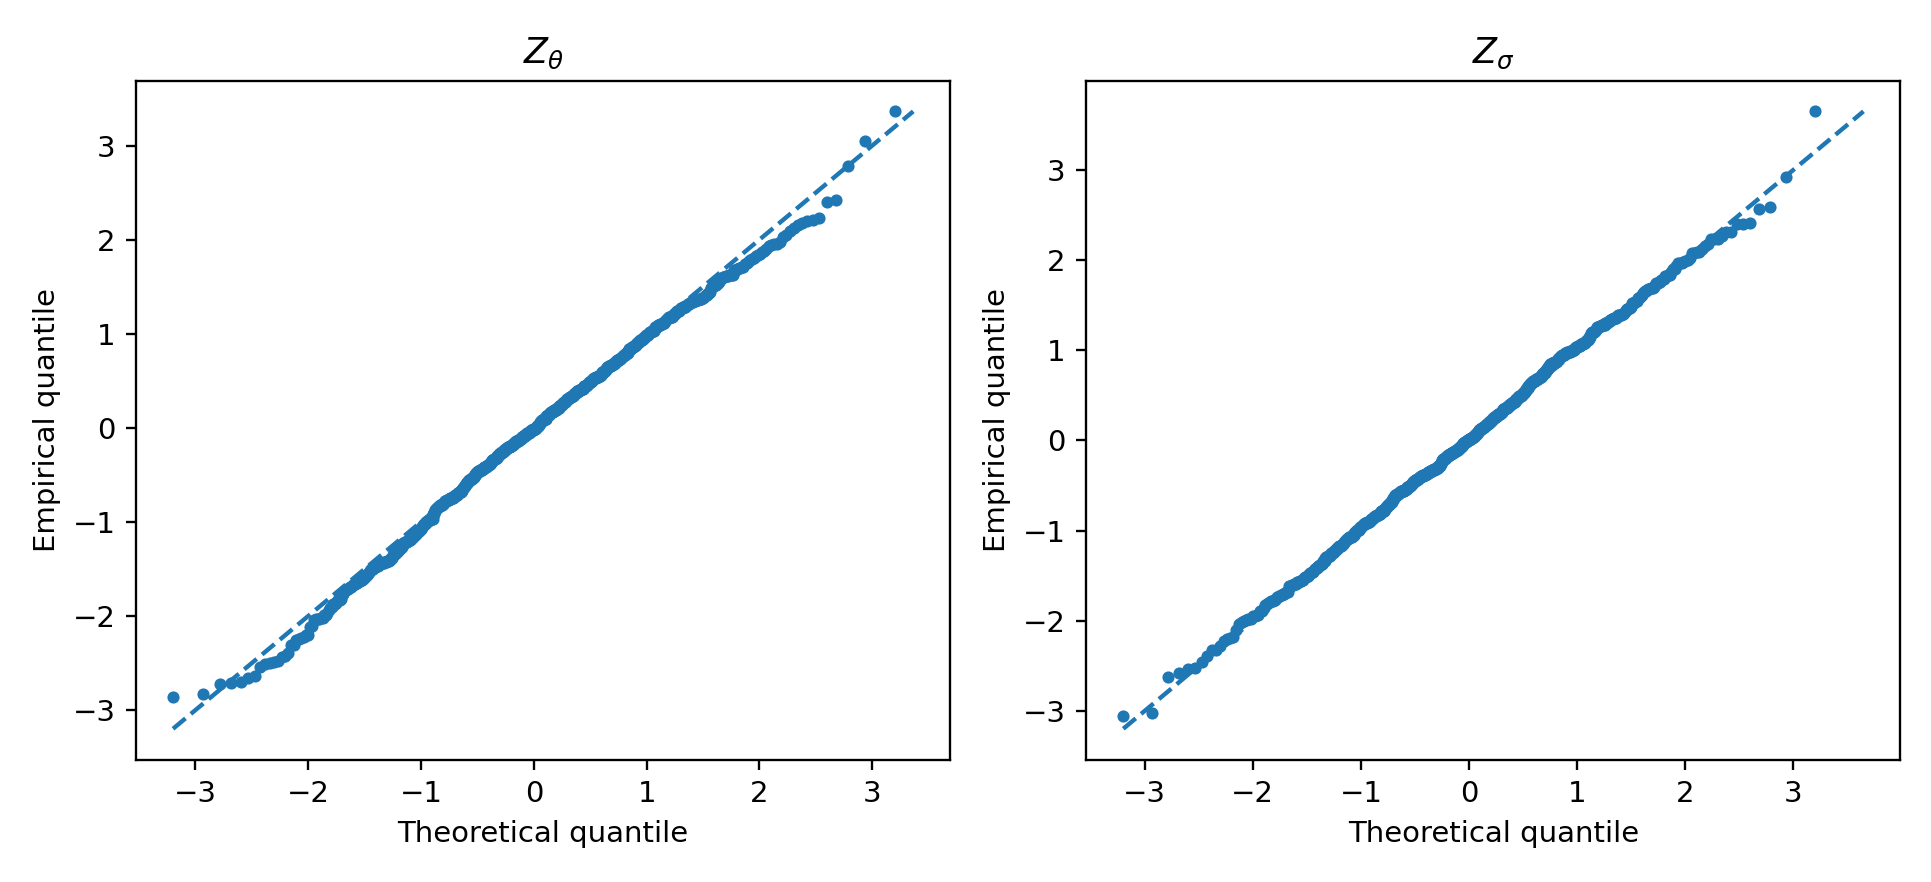
\includegraphics[width=.82\textwidth]{lan_qq_plots.png}
\caption{Normal quantile--quantile diagnostics for the standardised estimators. The visible right-skew of $Z_\theta$ at $N=5$ (skewness $0.49$, Kolmogorov--Smirnov $p=0.021$) dissipates along the design path ($p=0.42$ at $N=10$, $p=0.75$ at $N=20$), consistent with the first-order asymptotics.}
\label{fig:lan-qq}
\end{figure}

\subsection{Counterfactual process and bootstrap}

Fixed-intervention CDF sup-norm RMSE decreases from approximately $1.72\times10^{-3}$ to $2.13\times10^{-4}$. Distributional-effect sup-norm RMSE decreases from $1.64\times10^{-2}$ to $2.26\times10^{-3}$. Simultaneous coverage remains close to $0.95$ for both rate families.

\begin{table}[t]
\centering
\caption{Uniform target error and simultaneous coverage.}
\begin{tabular}{rrrrr}
\toprule
$N$ & CDF sup RMSE & Effect sup RMSE & Fast coverage & Slow coverage\\
\midrule
5  & $1.72\times10^{-3}$ & $1.64\times10^{-2}$ & 0.946 & 0.950\\
10 & $6.04\times10^{-4}$ & $6.29\times10^{-3}$ & 0.955 & 0.948\\
20 & $2.13\times10^{-4}$ & $2.26\times10^{-3}$ & 0.951 & 0.951\\
\bottomrule
\end{tabular}
\label{tab:coverage}
\end{table}

\begin{figure}[t]
\centering
\begin{subfigure}{.46\textwidth}
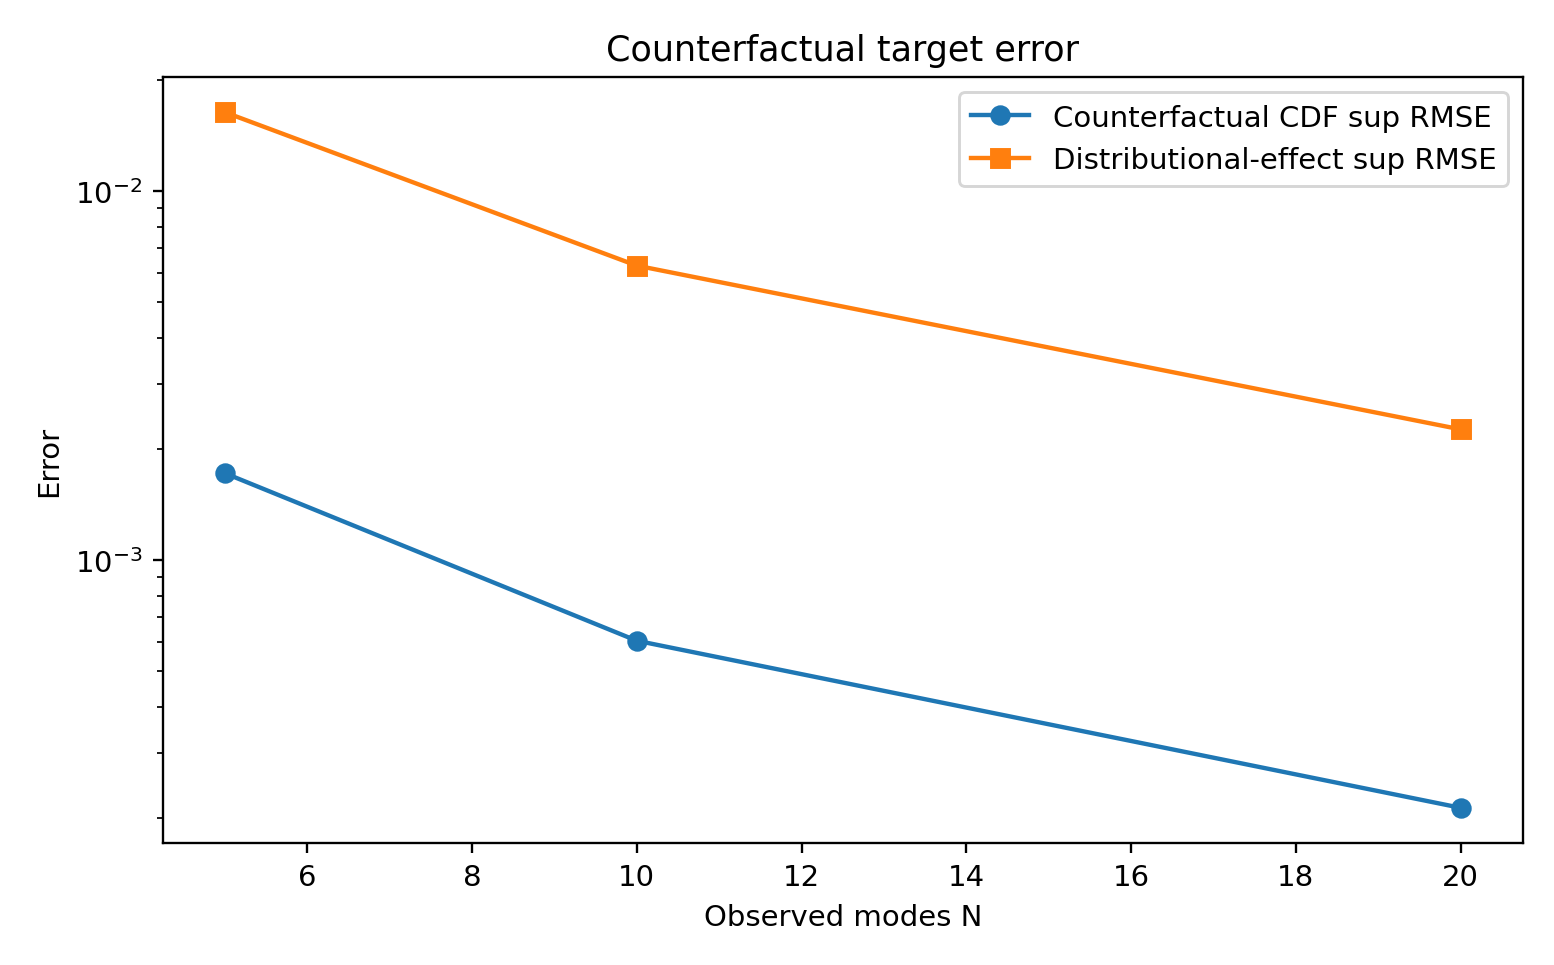
\includegraphics[width=\textwidth]{counterfactual_target_errors.png}
\caption{Uniform target errors.}
\end{subfigure}
\begin{subfigure}{.46\textwidth}
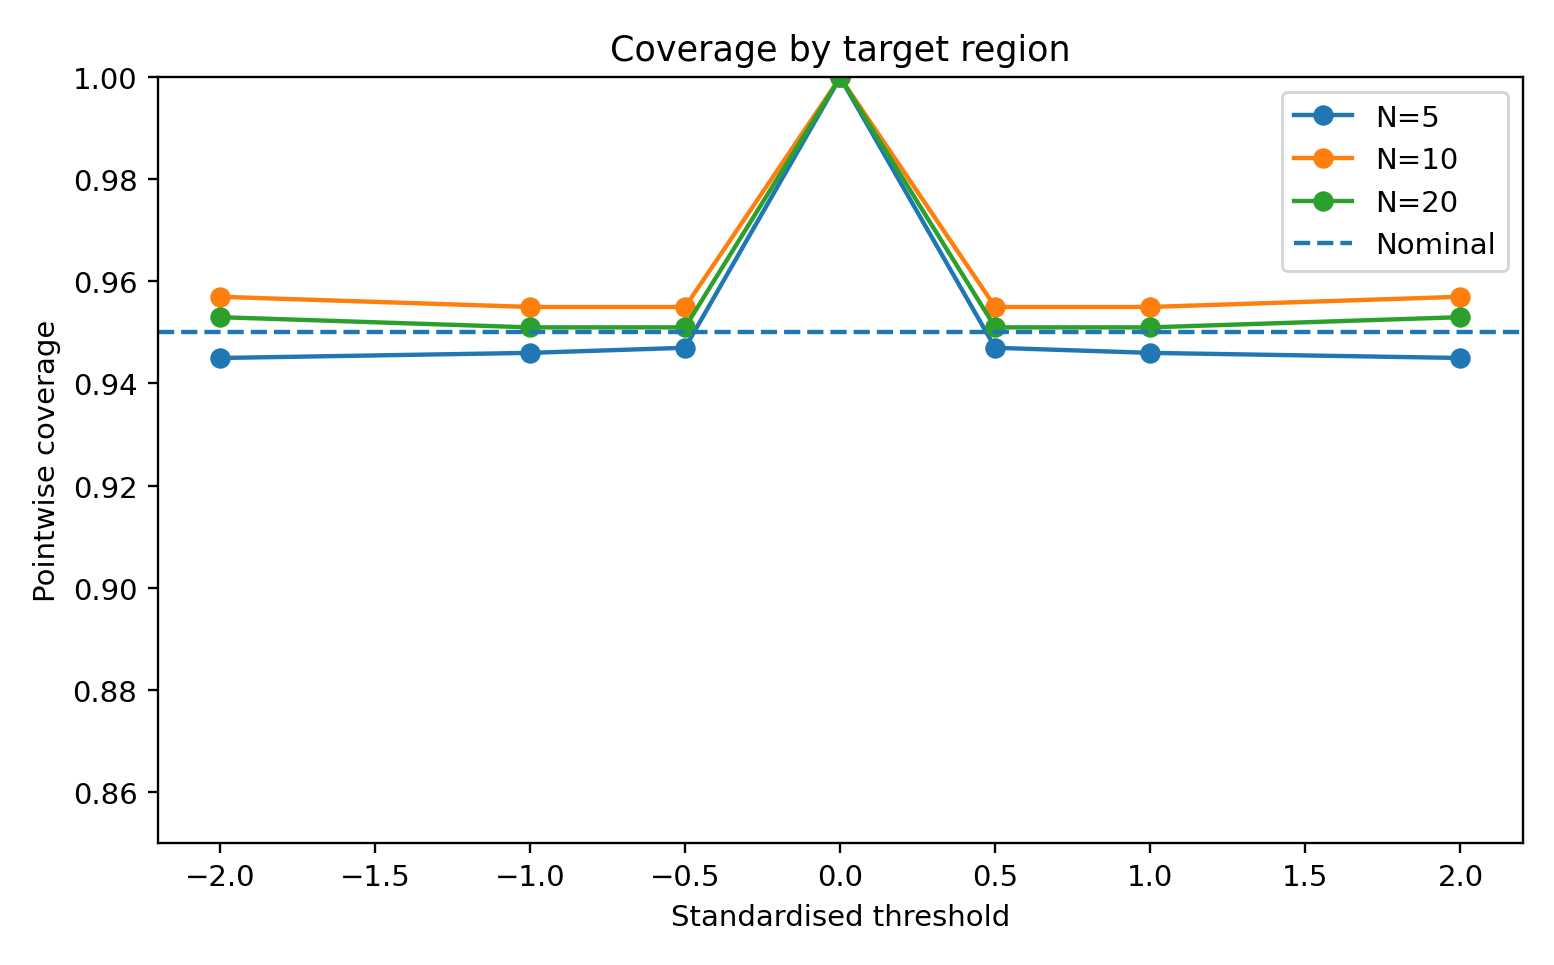
\includegraphics[width=\textwidth]{pointwise_coverage_by_threshold.png}
\caption{Coverage across thresholds.}
\end{subfigure}
\caption{Counterfactual target accuracy and coverage.}
\end{figure}

Beyond the headline coverage, the multiplier construction itself was stress-tested at $(N,n)=(10,8000)$ with $300$ replications per variant: the direct Gaussian draw, the modal-score multiplier with Gaussian weights, and the modal-score multiplier with Rademacher weights give statistically indistinguishable simultaneous coverage, and coverage is flat in the number of draws and in the threshold-grid resolution.

\begin{table}[t]
\centering
\caption{Bootstrap implementation sensitivity at $(N,n)=(10,8000)$, $300$ replications per row (Monte Carlo s.e.\ $\approx0.013$); nominal level $0.95$.}
\label{tab:boot-sens}
\begin{tabular}{llrrr}
\toprule
axis & variant & draws & fast cov. & slow cov.\\
\midrule
multiplier & direct Gaussian & 499 & 0.933 & 0.930\\
multiplier & modal Gaussian & 499 & 0.960 & 0.947\\
multiplier & modal Rademacher & 499 & 0.957 & 0.947\\
draws & direct Gaussian & 199 & 0.940 & 0.937\\
draws & direct Gaussian & 999 & 0.940 & 0.927\\
grid ($11$ pts) & direct Gaussian & 499 & 0.933 & 0.927\\
grid ($61$ pts) & direct Gaussian & 499 & 0.937 & 0.920\\
\bottomrule
\end{tabular}
\end{table}

\subsection{Approximation and sensitivity}

For the baseline spatial design, fitted log--log slopes are $-2.580$ for the mean tail, $-4.564$ for the variance tail, $-2.307$ for the strong RMS error, and $-2.580$ for the Gaussian CDF error, close to the theoretical values $-2.6,-4.6,-2.3,-2.6$. Temporal slopes lie between $0.994$ and $0.999$.

\begin{figure}[t]
\centering
\begin{subfigure}{.46\textwidth}
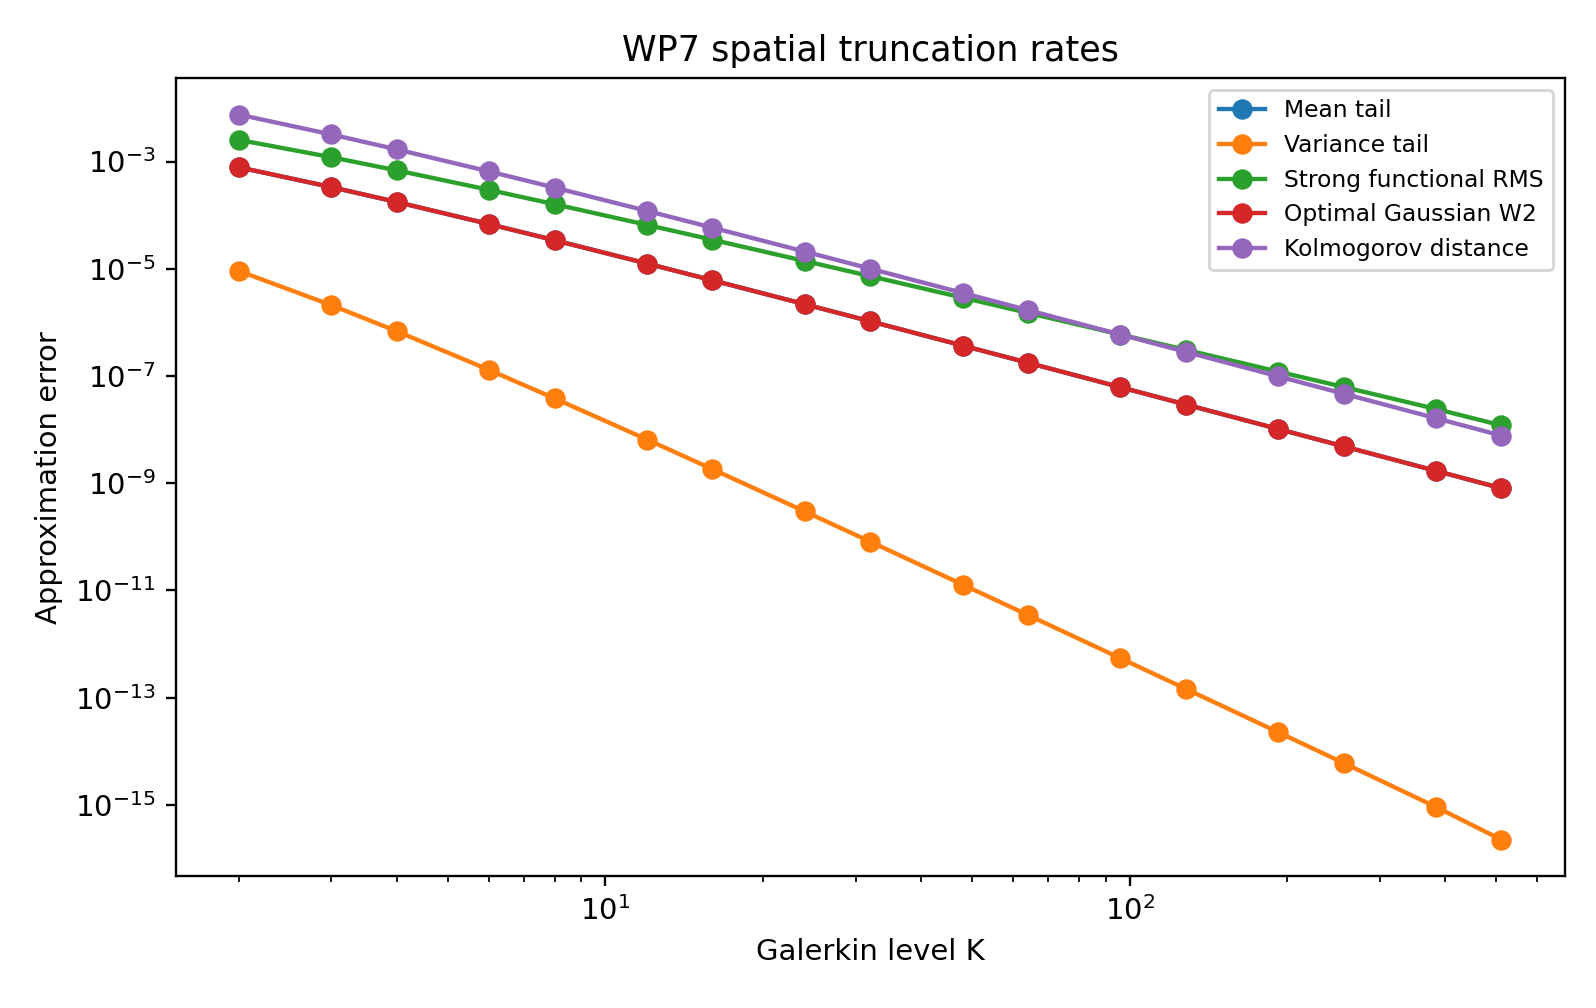
\includegraphics[width=\textwidth]{spatial_rates_baseline.png}
\caption{Galerkin rates.}
\end{subfigure}
\begin{subfigure}{.46\textwidth}
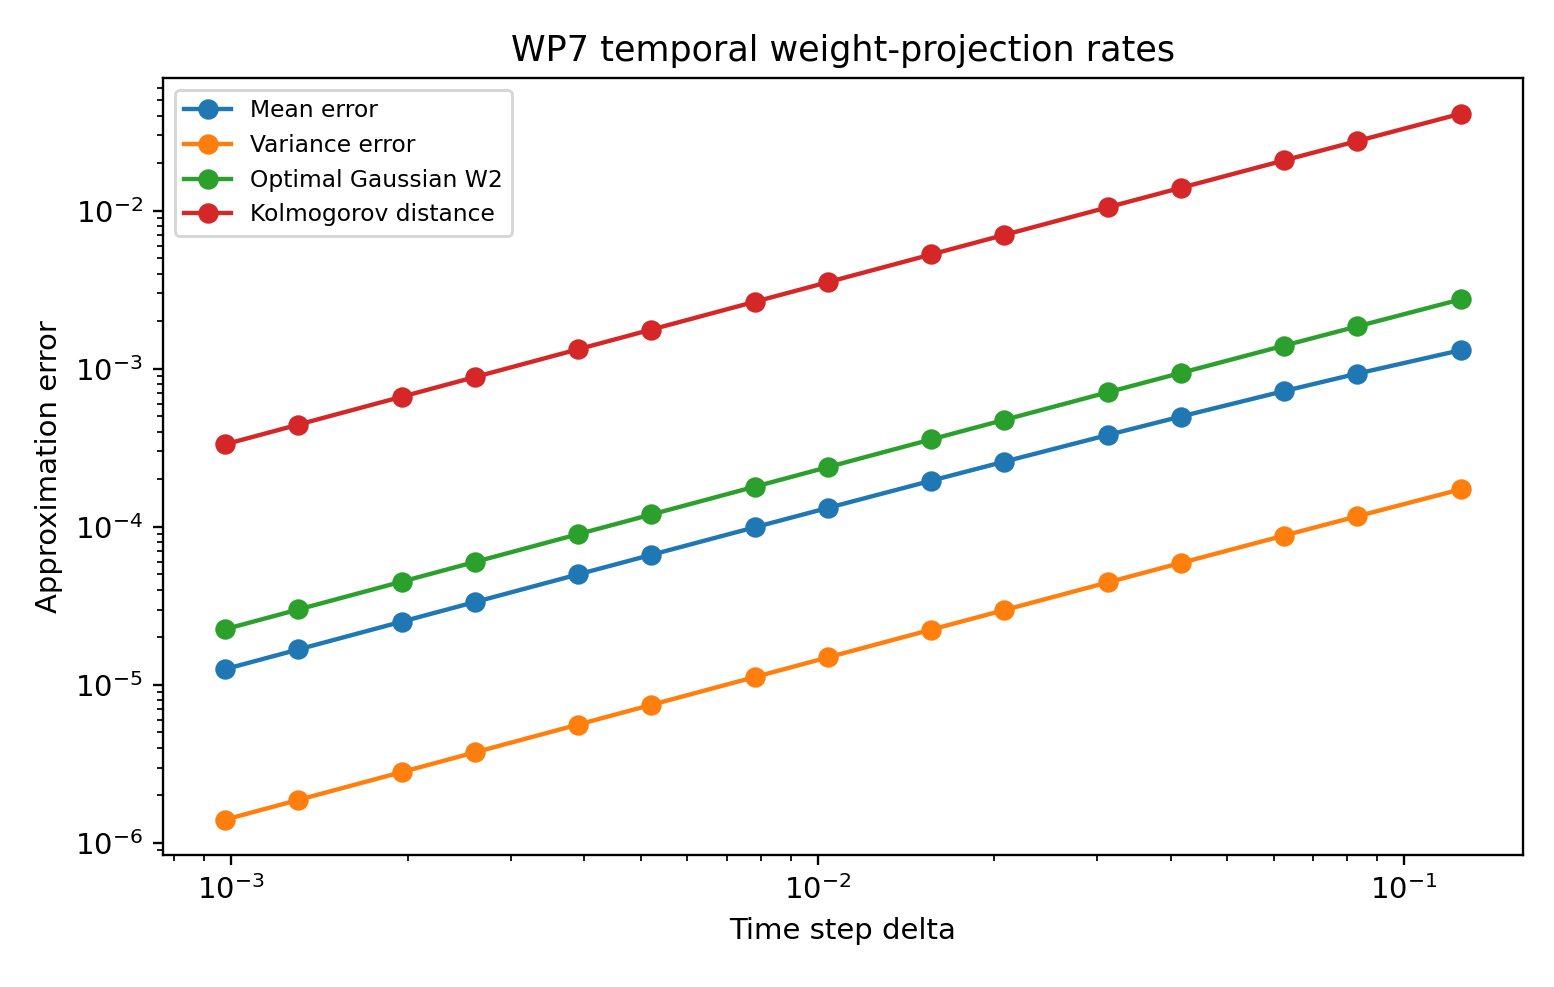
\includegraphics[width=\textwidth]{temporal_rates.png}
\caption{Temporal rates.}
\end{subfigure}
\caption{Deterministic approximation diagnostics.}
\end{figure}

For a non-commuting bounded perturbation, the central finite-difference derivative error decreases from $4.27\times10^{-6}$ at $\varepsilon=0.1$ to $1.71\times10^{-9}$ at $\varepsilon=0.002$. The CDF linearisation remainder is quadratic and the exact Gaussian $W_2$ distance remains below the derived Lipschitz envelope.

\subsection{Impossibility constructions}

The non-identification experiments are exact calculations rather than power studies. The adapted-feedback factual variance gap is zero while the post-intervention Kolmogorov distance is $0.0359$. The one-time open-loop factual variance gap is numerical zero and its post-intervention distance is $0.0984$. On a four-time grid, the factual covariance gap is $8.2\times10^{-16}$ while the post-intervention covariance gap is $0.7003$.


All tables and the headline diagnostics are regenerated by \texttt{make reproduce-publication}; the paper figures are regenerated end-to-end by the seeded validation pipeline (\texttt{make reproduce-paper}). The code records seeds, profiles, runtime, environment versions, and checksums.

\section{Discussion}

The paper places a narrow causal object on a complete mathematical and inferential footing. The intervention is an operator-module replacement inside a declared linear Gaussian SPDE class. The target is a counterfactual field-functional distribution. Identification is target specific. The inferential limit is mixed rate. Numerical approximation must be controlled at the target family's root-information scale.

Three distinctions are particularly important.

First, semantics and identification are separate. \Cref{sec:semantics} provides a coherent shared-noise intervention even before one asks whether the resulting law is recoverable from factual data; \Cref{sec:identification,sec:nonid} then characterise the positive and negative identification results.

Second, strong field approximation and Gaussian law approximation need not have the same rate. Under non-degeneracy, the variance tail enters normal CDF, quantile, and optimal Wasserstein comparisons linearly. Using the common-noise strong rate for every law target can be unnecessarily conservative.

Third, the phrase ``causal SPDE'' should not be read as unrestricted causal discovery. The intervention and invariant modules must be supplied. The feedback-gauge and open-loop constructions show that passive equality of factual laws cannot decide which part of a drift is the module that should be replaced.

Several extensions remain. Non-diagonal unbounded perturbations, including spatially varying divergence-form coefficients, require domain-sensitive perturbation theory. Semilinear equations require differentiability of nonlinear solution maps. Non-Gaussian noise calls for characteristic-function, Wasserstein, or quantile-specific methods rather than Gaussian mean--variance reduction. Physical-space observations require a separate statistical experiment and may produce different rates.

The present results are nevertheless sufficient for a coherent paper-level conclusion:
\begin{equation*}
\begin{aligned}
&\text{specified structural intervention}
+\text{identified factual experiment}\\
&\quad+\text{controlled numerical approximation}\\
&\hspace{2.5cm}\Longrightarrow
\text{uniformly inferable counterfactual laws}.
\end{aligned}
\end{equation*}
The impossibility results define the boundary of that conclusion rather than an exception to it.


\section*{Declarations}
\paragraph{Funding.} This work was supported by a DS4H (Digital Systems
for Humans) fellowship, Universit\'e C\^ote d'Azur.
\paragraph{Competing interests.} The author declares no competing interests.
\paragraph{Data and code availability.} All numerical results are generated
by the seeded replication package (Python reference implementation with a
Julia parity implementation, deterministic profiles, SHA-256 manifests, and
continuous-integration checks) archived with the manuscript sources; the
figures and tables of Section~\ref{sec:numerics} are reproduced end-to-end
by the documented \texttt{make} targets. [Repository DOI to be added upon
archival deposition.]
\paragraph{Acknowledgements.} Grammarly and generative AI tools were used
for proofreading, grammatical corrections, and targeted suggestions to
enhance sentence clarity. After using these tools, all authors reviewed and
edited the manuscript, taking full responsibility for its contents.

\bibliographystyle{plainnat}
\bibliography{references_merged}
\end{document}
"
% which silences the flags (status tracked in CHANGES_v2.md).
\ifdefined\SUBMISSIONCLEAN
\newcommand{\closuredraft}{}
\else
\newcommand{\closuredraft}{\par\smallskip\noindent
\textcolor{blue!55!black}{\footnotesize\textbf{[Verification
pending.]}}\par\smallskip}
\fi

\title{\textbf{Operator Interventions in Linear SPDEs:\\
Galerkin Structural Semantics, Mixed-Rate Local Asymptotic Normality,\\
and Uniform Inference for Post-Intervention Laws}}
\author{Gabriel Lucas St\'ephane Bontemps\thanks{Email:
\texttt{[address]}. ORCID: \texttt{[id]}.}\\[2pt]
{\normalsize GREDEG--CNRS, Universit\'e C\^ote d'Azur, Nice, France}\\
{\normalsize Adaptive Decision Lab, University of Oxford, Oxford, United Kingdom}}
\date{\ifdefined\SUBMISSIONCLEAN July 2026\else Working paper v4 (proto-submission draft), July 2026\fi}

\begin{document}
\maketitle

\begin{abstract}
We develop a causal-statistical theory for operator interventions in linear parabolic stochastic partial differential equations. The intervention replaces the generator coefficient while preserving the initial condition, noise spectrum, scale, observation mechanism, and primitive Wiener process. We first prove that the post-intervention SPDE is the infinite-dimensional limit of intervened Galerkin structural causal models driven by common exogenous Brownian segments. For Gaussian field functionals we give explicit post-intervention laws and necessary-and-sufficient target-identification criteria. Under exact discrete spectral observation, the likelihood is regular but anisotropic: the drift parameter is learned at rate $\sqrt{\sum_{k\le N}\lambda_k}$, whereas the noise scale is learned at rate $\sqrt{Nn}$. We establish local asymptotic normality, efficient estimation, uniform counterfactual CDF, quantile, tail, and distributional-effect processes, and feasible simultaneous confidence bands based on modal-score multipliers. We derive Fr\'echet derivatives of the operator-to-law map, combine statistical, Galerkin, temporal, and bounded operator-approximation errors, and state rate conditions for full-field inference. Finally, we construct observationally equivalent mechanisms with different post-intervention laws when forcing, initial, sensing, or cross-world modules are left unrestricted. Complete proofs are contained in the paper; numerical experiments verify the mixed rates, simultaneous coverage, approximation slopes, operator sensitivities, and impossibility constructions.
\end{abstract}

\noindent\textbf{Keywords:} stochastic partial differential equations; operator intervention; spectral inference; local asymptotic normality; empirical processes; multiplier bootstrap; Galerkin approximation.\\
\textbf{MSC2020:} 60H15; 62M05; 62F12; 62G15; 65M60.

% ---------- statements ----------
\section{Introduction}

Many scientific interventions change a law of motion rather than a scalar treatment. Diffusivity can be altered by a material, a boundary protocol can change a transport operator, and a spatial policy can modify the generator of a stochastic field. In these settings the object of interest is not merely a parameter. It is a post-intervention distribution of a functional of the field.

We study the linear parabolic model
\begin{equation}\label{eq:intro-spde}
 dU_t=\theta A_0U_t\,dt+\sigma Q^{1/2}dW_t,
 \qquad U_0=u_0,
\end{equation}
where $A_0$ is self-adjoint, negative, and has compact resolvent. The primary intervention is
\[
 \doop(\theta=\widetilde\theta),
\]
which replaces $\theta A_0$ by $\widetilde\theta A_0$ while leaving the other structural modules invariant. For a space-time weight $w$, the target is
\begin{equation}\label{eq:intro-target}
 F_{\widetilde\theta,w}(z;\vartheta)
 =\Pp_{\vartheta}\left\{
 \int_0^T\inner{w_t}{U_t^{\widetilde\theta}}\,dt\le z
 \right\},
 \qquad \vartheta=(\theta,\sigma).
\end{equation}

The paper addresses four distinct questions. First, what makes the formal replacement of an operator a structural intervention rather than a relabelled stochastic equation? Second, when is the counterfactual law identified from a factual observation experiment? Third, how can it be estimated uniformly over interventions, weights, and thresholds? Fourth, how do statistical and numerical errors interact at the inferential scale?

Our construction extends the finite-dimensional intervention logic of \citet{SokolHansen2014} to a diagonal parabolic SPDE. The post-intervention field is represented as the limit of intervened Galerkin structural causal models using the same Brownian path segments in every world. This common-noise convention is stronger than specifying marginal laws; it fixes the primitive disturbances that remain invariant under the intervention.

The statistical experiment uses exact discrete observations of the first $N$ spectral coordinates. This setting is close to the spectral inference literature surveyed by \citet{Cialenco2018}, but the target and asymptotic geometry are different. The exact transition likelihood produces two rates. With $\Lambda_N=\sum_{k\le N}\lambda_k$,
\[
 \sqrt{\Lambda_N}(\widehat\theta-\theta_0)
 \quad\text{and}\quad
 \sqrt{Nn}(\widehat\sigma-\sigma_0)
\]
have non-degenerate limits. Fixed absolute-intervention laws overwrite the factual drift and are therefore estimated at the faster scale rate. Factual and factual-versus-counterfactual effects retain the slower drift uncertainty.

The main contributions are as follows.

\begin{enumerate}[label=(\roman*)]
\item We prove exact finite-dimensional intervention semantics and uniform convergence of intervened Galerkin models to the post-intervention SPDE.
\item We give a fibre criterion for target identification and explicit finite-sample identification results under exact and noisy spectral observations.
\item We derive the exact likelihood, mixed Fisher-information limit, LAN expansion, efficient MLE, and moment convergence.
\item We establish uniform plug-in processes in $C(\cT)$, feasible multiplier bands, and contact-set tests for one-sided counterfactual hypotheses.
\item We prove operator-to-law derivatives for bounded perturbations and a separate analytic-semigroup theorem for the unbounded rescaling direction $A_0$.
\item We combine statistical, Galerkin, temporal, and operator approximation errors in one family-specific inference theorem.
\item We construct sharp non-identification examples. In particular, unrestricted feedback or open-loop forcing can absorb the factual operator and separate only after intervention.
\end{enumerate}

The contribution is deliberately narrower than causal discovery. The intervention is specified by the analyst. The theory identifies its target inside an admissible model class. It does not infer a causal graph from passive field observations, and it does not claim that every decomposition of an observed drift is structural.

\subsection*{Related literature}

Three literatures meet in this paper, and the delimitation matters.

\paragraph{Statistics for SPDEs.}
The spectral approach to drift estimation under continuous observation goes
back to \citet{HuebnerRozovskii1995}; see \citet{Lototsky2009} and the survey
of \citet{Cialenco2018}. An active recent strand studies discretely observed
parabolic equations: power variations and volatility estimation under
high-frequency sampling \citep{BibingerTrabs2020,Chong2020}, joint estimation
from space--time grids
\citep{HildebrandtTrabs2021,KainoUchida2021,TonakiKainoUchida2023,TonakiKainoUchida2024},
drift estimation from discretely sampled Fourier modes
\citep{CialencoDelgadoVencesKim2020}, local measurements
\citep{AltmeyerReiss2021}, and semilinear extensions
\citep{PasemannStannat2020}. Relative to this literature our observation
scheme is deliberately the cleanest one --- exact discrete observation of $N$
spectral coordinates --- but the output is of a different kind: a
\emph{joint} local asymptotic normality expansion with anisotropic diagonal
normalisation $\diag(\sqrt{\Lambda_N},\sqrt{Nn})$, efficiency and moment
convergence of the exact conditional MLE, pushed through to uniform
inference on post-intervention laws of field functionals. To our knowledge
both the mixed-rate LAN statement and any inferential theory for operator
interventions in SPDEs are new; the nearest discrete-observation results
concern estimation rates rather than experiment-level asymptotics.

\paragraph{Causal models for dynamical systems.}
Interventions in ODE systems were formalised as limits of structural
equation models by \citet{MooijJanzingScholkopf2013}, and extended to dynamic
equilibria and random differential equations by \citet{RubensteinEtAl2018}
and \citet{BongersMooij2018}; \citet{SokolHansen2014} treat SDEs via Euler
schemes, and \citet{PetersBauerPfister2022} survey the programme.
\Cref{thm:semantics} is the infinite-dimensional counterpart: the
post-intervention SPDE is the limit of intervened Galerkin structural causal
models driven by \emph{common} Brownian segments, so the intervention is
module surgery in the sense of \citet{Haavelmo1944} rather than a
relabelling of stochastic equations. The non-identification constructions of
\Cref{sec:nonid} calibrate exactly which invariances carry identifying
content.

\paragraph{Uniform inference on distributional targets.}
The plug-in processes and feasible bands use the functional delta method
\citep{vanDerVaart1998,vanDerVaartWellner1996}, multiplier approximations
for suprema \citep{ChernozhukovChetverikovKato2013}, directional
differentiability \citep{FangSantos2019}, and contact-set logic
\citep{AndrewsSoares2010,LintonSongWhang2010}. The finite-rank limit
geometry --- every target process is a deterministic derivative surface
loading a two-dimensional Gaussian --- makes these tools exact rather than
high-dimensional approximations, and the mixed rates propagate to
target-specific band widths. In econometric terms the targets are
counterfactual distributions and quantiles
\citep{ChernozhukovFernandezValMelly2013}; identification from discretely
sampled continuous-time dynamics connects to the aliasing literature
(\Cref{rem:no-aliasing}).

The paper is organised as follows. \Cref{sec:model} states the model and Gaussian target law. \Cref{sec:semantics} proves the intervention semantics. \Cref{sec:identification} treats identification. \Cref{sec:lan} develops the statistical experiment. \Cref{sec:uniform} gives uniform inference and bootstrap procedures. \Cref{sec:sensitivity} treats operator response and total error. \Cref{sec:nonid} gives the impossibility boundary. \Cref{sec:numerics} reports numerical validation. \ifdefined\MERGEDDOC Complete proofs of every statement are collected in \Cref{sec:proofs} (parts S0--S8), in dependency order and preceded by part S0, which restates every imported external theorem as an attributed local proposition whose hypotheses are verified at each point of use.\else Complete proofs of every statement are collected in the accompanying consolidated technical supplement (parts S0--S8), which supersedes the separate work-package archives; part S0 restates every imported external theorem as an attributed local proposition whose hypotheses are verified at each point of use.\fi

\subsection*{Notation}
$H=L^2(D)$ with inner product $\inner\cdot\cdot$ and norm $\norm\cdot$; $A_0$ is self-adjoint, negative, with compact resolvent, eigenpairs $(-\lambda_k,e_k)$, $0<\lambda_1\le\lambda_2\le\cdots$, and $\lambda_k\asymp k^{2/d}$ (Weyl growth). $\Lambda_N:=\sum_{k\le N}\lambda_k$. The parameter is $\vartheta=(\theta,\sigma)$, its true value $\vartheta_0$, and $A_{N,n}:=\diag(\sqrt{\Lambda_N},\sqrt{Nn})$ is the information normalisation. $\doop(\theta=\tilde a)$ denotes module surgery on the generator coefficient. Weak convergence is $\Rightarrow$; $\op(1),\Op(1)$ are stochastic order symbols; $C,c$ denote finite positive constants that may change between displays and whose dependencies are stated where they matter; $a\wedge b=\min(a,b)$, $a\vee b=\max(a,b)$, and $x_+=\max(x,0)$. For a compact index set $\cT$, $C(\cT)$ carries the supremum norm $\norm\cdot_\infty$. \ifdefined\MERGEDDOC\else \Cref{tab:crosswalk} maps each statement to its proof.\fi

\ifdefined\MERGEDDOC\else
\begin{table}[t]
\centering\small
\caption{Statement-to-proof crosswalk\ifdefined\MERGEDDOC\ (\Cref{sec:proofs})\else\ (technical supplement)\fi.}
\label{tab:crosswalk}
\begin{tabular}{ll}
\toprule
Main-text statement & Proof location \\
\midrule
\Cref{prop:gaussian-law} & Part S2 (Gaussian post-intervention law)\\
\Cref{prop:exact-scm,thm:semantics} & Part S1 (exact representation; Galerkin limits)\\
\Cref{thm:fibre,thm:exact-id,prop:partial} & Part S2 (identification)\\
\Cref{thm:lan} & Part S3 (LAN, efficiency, moment convergence)\\
\Cref{thm:processes,thm:quantile-tail} & Part S4 (uniform target processes)\\
\Cref{thm:bands} & Part S5 (multiplier, floor bands, contact sets)\\
\Cref{thm:sensitivity} & Part S6 (operator sensitivity)\\
\Cref{thm:total-error} & Part S7 (total error)\\
\Cref{thm:gauge-main,thm:nonid-assembly} & Part S8 (non-identification)\\
\bottomrule
\end{tabular}
\end{table}
\fi

\section{Model and counterfactual targets}\label{sec:model}

Let $D\subset\R^d$ be bounded and regular, and let $H=L^2(D)$. Let $A_0:D(A_0)\subset H\to H$ be densely defined, self-adjoint, negative, and have compact resolvent. There is an orthonormal basis $(e_k)_{k\ge1}$ and eigenvalues $0<\lambda_1\le\lambda_2\le\cdots$ such that
\[
 A_0e_k=-\lambda_ke_k,
 \qquad
 \lambda_k\asymp k^{2/d}.
\]
Let $W_t=\sum_{k\ge1}\beta_k(t)e_k$ be cylindrical Wiener noise and let $Q^{1/2}e_k=q_ke_k$.

\begin{assumption}[Positive core]\label{ass:core}
The factual parameter belongs to a compact rectangle
\[
 \vartheta=(\theta,\sigma)\in
 [\underline\theta,\overline\theta]\times
 [\underline\sigma,\overline\sigma]\Subset(0,\infty)^2.
\]
The intervention set $\widetilde\Theta$ is a compact subset of $(0,\infty)$. The initial state is deterministic. At minimum,
\[
 \sum_{k\ge1}\frac{q_k^2}{\lambda_k}<\infty.
\]
For pathwise Galerkin rates we impose the stronger fractional summability stated in \Cref{sec:semantics}.
\end{assumption}

The factual mild solution is
\[
 U_t^\theta
 =e^{t\theta A_0}u_0
 +\sigma\int_0^t e^{(t-s)\theta A_0}Q^{1/2}dW_s.
\]
The intervention replaces only the generator coefficient:
\begin{equation}\label{eq:cf-spde}
 dU_t^{a}=aA_0U_t^{a}\,dt+\sigma Q^{1/2}dW_t,
 \qquad U_0^a=u_0,
 \qquad a\in\widetilde\Theta.
\end{equation}
All fields in \eqref{eq:cf-spde} are constructed with the same $u_0,Q,\sigma$, and $W$.

For $w\in L^2(0,T;H)$ define
\[
 \Psi_w(U)=\int_0^T\inner{w_t}{U_t}\,dt.
\]
Write $w_k(t)=\inner{w_t}{e_k}$ and $u_{0,k}=\inner{u_0}{e_k}$. The law of $\Psi_w(U^a)$ is obtained in three displayed steps. Modally, $u^a_k(t)=e^{-a\lambda_kt}u_{0,k}+\sigma q_k\int_0^te^{-a\lambda_k(t-s)}d\beta_k(s)$, so
\[
 \Psi_w(U^a)
 =\sum_{k\ge1}\int_0^Tw_k(t)u^a_k(t)\,dt
 =m_a(w)+\sigma\sum_{k\ge1}q_k\int_0^T\!\!w_k(t)\!\int_0^t
 e^{-a\lambda_k(t-s)}\,d\beta_k(s)\,dt .
\]
The stochastic Fubini interchange (Part S0, imported stochastic Fubini theorem) applies because
\[
 \int_0^T\Big(\E\int_0^T w_k(t)^2e^{-2a\lambda_k(t-s)}\mathbf 1_{s\le t}\,dt\Big)^{1/2}ds
 \le\sqrt T\,\norm{w_k}_{L^2}<\infty
 \qquad\text{for each }k,
\]
and exchanging the two integrals collects, for each innovation time $s$, the total future weight it loads:
\[
 \int_0^T\!\!w_k(t)\!\int_0^te^{-a\lambda_k(t-s)}d\beta_k(s)\,dt
 =\int_0^T\Big(\underbrace{\int_s^Tw_k(t)e^{-a\lambda_k(t-s)}\,dt}_{=\,g_{a,k,w}(s)}\Big)d\beta_k(s).
\]
Hence
\[
 \Psi_w(U^a)
 =m_a(w)+\sigma\sum_{k\ge1}q_k
 \int_0^T g_{a,k,w}(s)\,d\beta_k(s),
\]
where
\begin{align}
 m_a(w)
 &=\sum_{k\ge1}u_{0,k}\int_0^T w_k(t)e^{-a\lambda_kt}\,dt,\label{eq:mean}\\
 g_{a,k,w}(s)
 &=\int_s^T w_k(t)e^{-a\lambda_k(t-s)}\,dt.\label{eq:transfer}
\end{align}

\begin{proposition}[Gaussian counterfactual law]\label{prop:gaussian-law}
Under \Cref{ass:core},
\[
 \Psi_w(U^a)\sim N\bigl(m_a(w),\sigma^2V_a(w)\bigr),
\]
where
\begin{equation}\label{eq:variance}
 V_a(w)=\sum_{k\ge1}q_k^2\int_0^T g_{a,k,w}(s)^2\,ds.
\end{equation}
Consequently,
\[
 F_{a,w}(z;\sigma)
 =\Phi\left(
 \frac{z-m_a(w)}{\sigma\sqrt{V_a(w)}}
 \right).
\]
\end{proposition}

\inwords{The intervention law is explicit once the invariant structural modules are fixed. The factual drift parameter $\theta$ is absent from the fixed absolute-intervention law because it has been overwritten.}

The indexed target set is
\[
 \cT=\widetilde\Theta\times\cW\times\cZ,
\]
where $\cZ$ is compact and $\cW$ is a compact ellipsoid in a space-time Sobolev basis. For CDF and quantile inference we impose
\[
 \inf_{(a,w)\in\widetilde\Theta\times\cW}V_a(w)>0.
\]
Wasserstein and field-functional convergence do not require this non-degeneracy condition.

\begin{figure}[t]
\centering
\resizebox{.96\textwidth}{!}{% Modal decay under intervention and the transfer kernel g_{a,k,w}.
% Left: e^{-a lambda_k t} for factual theta vs intervened a on two modes.
% Right: the backward transfer kernel s -> g_{a,k,w}(s) for w_k = 1.
\begin{tikzpicture}[font=\small, scale=1.0,
  ax/.style={-{Stealth[length=2.2mm]}, thick},
  lbl/.style={font=\footnotesize\itshape, text=black!70}]
% ---------------- left panel: modal decay ----------------
\begin{scope}
\draw[ax] (0,0) -- (4.4,0) node[below left=1pt]{$t$};
\draw[ax] (0,0) -- (0,3.1);
\node[anchor=south, rotate=90] at (-.55,1.4) {$e^{-a\lambda_k t}$};
\draw (0.03,2.6) node[left, font=\scriptsize]{$1$} -- (-0.07,2.6);
% mode k=1: lambda=1 scaled; factual theta=0.7 -> rate .7; intervened a=1.4
\draw[thick, blue!60!black]  plot[domain=0:4, samples=60] (\x,{2.6*exp(-0.55*\x)});
\draw[thick, red!60!black, dashed] plot[domain=0:4, samples=60] (\x,{2.6*exp(-1.1*\x)});
% mode k=2: lambda 4x
\draw[thin, blue!60!black]  plot[domain=0:4, samples=60] (\x,{2.6*exp(-2.2*\x)});
\draw[thin, red!60!black, dashed] plot[domain=0:4, samples=60] (\x,{2.6*exp(-4.4*\x)});
\node[lbl, blue!60!black]  at (3.05,1.15) {factual $\theta$};
\node[lbl, red!60!black]   at (2.95,0.33) {intervened $\tilde a=2\theta$};
\node[lbl] at (2.2,-0.42) {mode $k=1$ (thick), $k=2$ (thin): $\lambda_2=4\lambda_1$};
\end{scope}
% ---------------- right panel: transfer kernel ----------------
\begin{scope}[xshift=7.1cm]
\draw[ax] (0,0) -- (4.4,0) node[below left=1pt]{$s$};
\draw[ax] (0,0) -- (0,3.1);
\node[anchor=south, rotate=90] at (-.55,1.4) {$g_{a,k,w}(s)$};
\draw (4.0,0.05) -- (4.0,-0.05) node[below, font=\scriptsize]{$T$};
% g(s) = (1 - e^{-a lambda (T-s)})/(a lambda) for w=1; a*lambda = .55 resp 1.1 (k=1)
\draw[thick, blue!60!black] plot[domain=0:4, samples=60]
  (\x,{2.6*(1-exp(-0.55*(4-\x)))/(0.55*4)*2.2});
\draw[thick, red!60!black, dashed] plot[domain=0:4, samples=60]
  (\x,{2.6*(1-exp(-1.1*(4-\x)))/(1.1*4)*2.2});
\node[lbl, align=left, anchor=west] at (1.45,2.85)
  {$g_{a,k,w}(s)=\int_s^T w_k(t)e^{-a\lambda_k(t-s)}\,dt$\\[1pt]
   here $w_k\equiv1$: $g=\frac{1-e^{-a\lambda_k(T-s)}}{a\lambda_k}$};
\node[lbl, blue!60!black] at (1.15,1.28) {$a=\theta$};
\node[lbl, red!60!black]  at (1.28,0.44) {$a=\tilde a$};
\node[lbl, align=center] at (2.2,-0.42)
  {$V_a(w)=\sum_kq_k^2\!\int_0^T\!g_{a,k,w}^2$: intervention lowers the\\
   load of every innovation, monotonically in $a$};
\end{scope}
\end{tikzpicture}
}
\caption{The two ingredients of the post-intervention law. Left: modal decay $e^{-a\lambda_kt}$ under the factual coefficient and under $\doop(\theta=\tilde a)$, for a slow and a fast mode. Right: the backward transfer kernel $g_{a,k,w}$ collecting, for each innovation time $s$, the future weight it loads; by It\^o isometry the target variance is $\sigma^2\sum_kq_k^2\norm{g_{a,k,w}}_{L^2}^2$.}
\label{fig:transfer}
\end{figure}

\section{Galerkin structural intervention semantics}\label{sec:semantics}

Let $H_K=\operatorname{span}\{e_1,\ldots,e_K\}$ and let $P_K$ be the orthogonal projection. Fix a partition $0=t_0<\cdots<t_J=T$. For mode $k$ and interval $j$, use the Brownian segment
\[
 E_{k,j}(r)=\beta_k(t_j+r)-\beta_k(t_j),
 \qquad 0\le r\le\Delta_j,
\]
as the primitive exogenous variable.

For $a>0$, define the exact local map
\[
 G_{a,k,r}(x,e)
 =e^{-a\lambda_kr}x
 +\sigma q_k\mathfrak I_{a\lambda_k,r}(e),
\]
where
\begin{equation}\label{eq:pathmap}
 \mathfrak I_{c,r}(e)
 =e(r)-c\int_0^r e^{-c(r-s)}e(s)\,ds.
\end{equation}
The map in \eqref{eq:pathmap} is continuous on $C_0([0,r])$. For Brownian $e$ it equals the It\^o convolution
\[
 \int_0^r e^{-c(r-s)}de(s)
\]
by integration by parts. Thus the structural equation is a measurable, indeed continuous, function of the primitive Brownian segment.

The finite model recursively applies $G_{a,k,r}$ to every mode and interval. The intervention $\doop(\theta=a)$ replaces the family $G_{\theta,k,r}$ by $G_{a,k,r}$ while preserving all exogenous segments.

\begin{proposition}[Exact structural representation]\label{prop:exact-scm}
For every $K$, partition, and $a\in\widetilde\Theta$, the intervened structural recursion equals the exact projected post-intervention SPDE path:
\[
 \mathcal X_t^{K,\doop(\theta=a)}
 =U_t^{K,a}
 =P_KU_t^a
 \quad\text{for all }t\in[0,T]
 \quad\text{almost surely}.
\]
\end{proposition}

\begin{theorem}[Galerkin limits of intervened SCMs]\label{thm:semantics}
Assume, for some $\alpha\ge0$ and $\delta>0$,
\[
 u_0\in D((-A_0)^\alpha),
 \qquad
 \sum_{k\ge1}q_k^2\lambda_k^{2(\alpha+\delta)-1}<\infty.
\]
Then
\[
 \sup_{a\in\widetilde\Theta}
 \E\sup_{t\le T}
 \norm{U_t^a-P_KU_t^a}_H^2
 \le C\lambda_{K+1}^{-2\alpha}.
\]
Under only $u_0\in H$ and $\sum q_k^2/\lambda_k<\infty$,
\[
 \sup_a\E\int_0^T\norm{U_t^a-P_KU_t^a}^2dt\to0.
\]
Finally, for every bounded $\cW\subset L^2(0,T;H)$,
\[
 \sup_{a,w}
 \E\abs{\Psi_w(U^a)-\Psi_w(P_KU^a)}^2\to0,
\]
and the corresponding laws converge uniformly in quadratic Wasserstein distance.
\end{theorem}

\inwords{The post-intervention SPDE is not introduced by notation alone. It is the limit of finite structural models whose operator mechanism is surgically replaced while the primitive shocks are fixed. \Cref{fig:modules} displays the two-world construction.}

\begin{figure}[t]
\centering
\resizebox{.98\textwidth}{!}{% Two-world common-noise construction. Design rules: one box per concept,
% at most one short label per arrow, labels never over lines or boxes.
\begin{tikzpicture}[
  font=\small,
  box/.style={draw, rounded corners=2pt, minimum width=3.4cm,
              minimum height=1.05cm, align=center},
  shared/.style={box, fill=gray!16, minimum width=3.9cm, minimum height=1.7cm},
  mechF/.style={box, fill=blue!10},
  mechI/.style={box, fill=red!9},
  law/.style={box, fill=green!11},
  flow/.style={-{Stealth[length=2.6mm]}, semithick},
  surg/.style={-{Stealth[length=3mm]}, very thick, red!70!black},
  lbl/.style={font=\footnotesize\itshape, text=black!70}
]
% shared primitives: one box
\node[shared] (prim) at (0,-2.2)
  {invariant modules\\[2pt]
   $W,\quad u_0,\quad Q^{1/2},\quad \sigma,\quad \mathcal H$};

% factual row (y=0)
\node[mechF] (Gf) at (5.4,0)  {mechanism\\[-1pt] $dU=\theta A_0U\,dt+\sigma Q^{1/2}dW$};
\node[box]   (Uf) at (10.4,0) {field $U^{\theta}$};
\node[law]   (Yf) at (14.6,0) {observed law\\[-1pt] $Y_{k,j}=u_k(t_j)$};

% intervened row (y=-4.4)
\node[mechI] (Gi) at (5.4,-4.4)  {mechanism\\[-1pt] $dU=\tilde aA_0U\,dt+\sigma Q^{1/2}dW$};
\node[box]   (Ui) at (10.4,-4.4) {field $U^{\tilde a}$};
\node[law]   (Ti) at (14.6,-4.4) {target law\\[-1pt] $F_{\tilde a,w}$};

% shared -> mechanisms (two clean diagonals from box corners)
\draw[flow] (prim.north east) -- (Gf.west);
\draw[flow] (prim.south east) -- (Gi.west);
\node[lbl, anchor=north] at (2.15,-4.45) {same Brownian segments};

% rows
\draw[flow] (Gf) -- (Uf);
\draw[flow] (Uf) -- (Yf);
\draw[flow] (Gi) -- (Ui);
\draw[flow] (Ui) -- (Ti);
\node[lbl] at (12.5,0.72)  {spectral sampling};
\node[lbl] at (12.5,-3.68) {functional $\Psi_w$};

% surgery arrow, label fully to its left in white space
\draw[surg] (Gf.south) -- (Gi.north);
\node[font=\footnotesize, red!70!black, align=right, anchor=east] at (4.55,-2.2)
  {$\doop(\theta=\tilde a)$};

% estimation arrow on the far right, label to its right
\draw[flow, dashed, black!60] (Yf.south) -- (Ti.north);
\node[lbl, anchor=west, align=left] at (15.8,-2.2)
  {plug-in $\widehat\vartheta$\\ rates $\sqrt{\Lambda_N}$, $\sqrt{Nn}$};

% Galerkin note in free space between the field boxes
\node[lbl] at (10.4,-2.2)
  {$\mathcal X^{K,\doop(\theta=\tilde a)}=P_KU^{\tilde a}\ \xrightarrow{\ K\to\infty\ }\ U^{\tilde a}$};
\end{tikzpicture}
}
\caption{Common-noise structural semantics. The invariant modules (left) feed both worlds; $\doop(\theta=\tilde a)$ replaces only the generator mechanism. The observed spectral law identifies $\widehat\vartheta$, which is transported to the target law along the dashed edge at the mixed rates of \Cref{sec:lan}.}
\label{fig:modules}
\end{figure}

\begin{remark}[Relation to finite-dimensional intervention limits]\label{rem:sde-analogue}
For SDEs, \citet{SokolHansen2014} obtain the post-intervention equation as the limit of intervened Euler-scheme structural models; ODE precursors are \citet{MooijJanzingScholkopf2013,RubensteinEtAl2018}. Two features distinguish the present construction: the finite recursion is \emph{exact} (no scheme error enters the semantics, cf.\ the transfer principle closing this section), and the limit is taken in the spatial resolution $K$ rather than in a time step, which is what makes the common-noise coupling compatible with the spectral statistical experiment of \Cref{sec:lan}.
\end{remark}

\begin{remark}[Regularity margin]
The boundary condition
\[
 \sum_kq_k^2\lambda_k^{2\alpha-1}<\infty
\]
controls fixed-time fractional regularity but does not by itself justify the stated supremum-in-time $L^2$ maximal estimate. The positive margin $\delta$ is a clean factorisation condition in the sense of the factorisation method of \citet{DaPratoKwapienZabczyk1987}. For one-dimensional space-time white noise it implies $\alpha+\delta<1/4$.
\end{remark}

The exact recursion has no temporal approximation error. Such an error appears only when $G_{a,k,r}$ is replaced by an Euler or other numerical map. This distinction becomes important in \Cref{sec:sensitivity}.

\section{Target identification}\label{sec:identification}

Identification is a property of the target, observation experiment, and admissible mechanism class. Let $P_\vartheta^Y$ denote the factual observed law and let $T_\tau(\vartheta)$ denote a counterfactual target.

\begin{lemma}[Fibre criterion]\label{thm:fibre}
The target $T_\tau$ is identified from $P_\vartheta^Y$ if and only if
\[
 P_{\vartheta_1}^Y=P_{\vartheta_2}^Y
 \quad\Longrightarrow\quad
 T_\tau(\vartheta_1)=T_\tau(\vartheta_2)
\]
for every pair $\vartheta_1,\vartheta_2$ in the admissible model.
\end{lemma}

This elementary observation is stated as a lemma because its value is organisational rather than technical: it separates necessary-and-sufficient logic from convenient sufficient conditions. We now specialise it to spectral observations.

Let $t_j=j\Delta$, and observe
\[
 Y_{k,j}=u_k(t_j),
 \qquad k=1,\ldots,N.
\]
For each mode,
\begin{equation}\label{eq:transition}
 Y_{k,j+1}\mid Y_{k,j}
 \sim N\left(\rho_k(\theta)Y_{k,j},\eta_k^2(\theta,\sigma)\right),
\end{equation}
where
\[
 \rho_k(\theta)=e^{-\theta\lambda_k\Delta},
 \qquad
 \eta_k^2(\theta,\sigma)
 =\sigma^2q_k^2\frac{1-e^{-2\theta\lambda_k\Delta}}{2\theta\lambda_k}.
\]

\begin{theorem}[Exact finite-sample spectral identification]\label{thm:exact-id}
Suppose an observed mode satisfies $q_k>0$ and is observed at $0,\Delta,2\Delta$. Equality of its finite-dimensional law identifies
\[
 \rho_k
 =\frac{\Cov(Y_{k,1},Y_{k,2})}{\Var(Y_{k,1})},
 \qquad
 \theta=-\frac{\log\rho_k}{\lambda_k\Delta},
\]
and then identifies $\sigma$ from $\Var(Y_{k,1})$. Hence $(\theta,\sigma)$ and every fixed-intervention target are identified.
\end{theorem}

With only one positive-time observation, full identification still holds if an observed initial coordinate is non-zero or if at least two distinct eigenvalues are observed. If all observed initial coordinates vanish and only one repeated eigenvalue is present, the data identify the composite scale $\sigma^2h_\lambda(\theta)$ rather than the two parameters separately.

\begin{remark}[No aliasing]\label{rem:no-aliasing}
Identification of $\theta$ from $\rho_k=e^{-\theta\lambda_k\Delta}$ exploits positivity and reality of the semigroup spectrum: on the positive core, the discrete transition determines the continuous-time generator uniquely. This contrasts with the aliasing problem for general finite-parameter continuous-time systems observed at equally spaced times \citep{Phillips1973,HansenSargent1983}, in which distinct generators are compatible with the same discrete-time law.
\end{remark}

For a fixed absolute intervention, the law in \Cref{prop:gaussian-law} depends on $\sigma$ but not on the overwritten factual $\theta$. Thus a non-degenerate fixed-intervention target can remain identified even when the full factual parameter is not.

For noisy observations
\[
 \widetilde Y_{k,j}=Y_{k,j}+\varepsilon_{k,j},
\]
a known error law with non-vanishing characteristic function identifies the latent finite-dimensional law by deconvolution. In the Gaussian state-space model, two positive observation times identify $(\theta,\sigma)$ when the measurement variance is known; three positive times identify an unknown constant measurement variance as well.

For a general linear sensor $Y=\mathcal HU$, the mean and covariance must be treated separately. Let $\mathfrak M_\theta$ map an initial direction to its observed mean trajectory and let $\mathfrak K_\theta$ map a covariance input to the observed covariance kernel. Let $\mathfrak L_{a,w}$ and $\mathfrak V_{a,w}$ be the corresponding target maps.

\begin{proposition}[Partial-observation kernel criterion]\label{prop:partial}
A Gaussian target is identified on a linear nuisance class if and only if
\[
 \ker\mathfrak M_\theta\subseteq\ker\mathfrak L_{a,w}
 \quad\text{and}\quad
 \ker\mathfrak K_\theta\subseteq\ker\mathfrak V_{a,w}.
\]
Ordinary state observability controls the mean component. Covariance identification is a lifted operator problem and does not follow automatically from state observability.
\end{proposition}

A simple modal support condition becomes necessary only in an enlarged model with free mode-specific amplitudes. In the scalar positive core, known $Q$ links unobserved modes through the common $\sigma$, so observing every target mode is not necessary.

\section{Exact likelihood, mixed-rate LAN, and efficiency}\label{sec:lan}

Let $\mathcal E_{N,n}$ be the experiment generated by the transitions in \eqref{eq:transition}. Conditional on the initial values, the log-likelihood is
\[
 \ell_{N,n}(\theta,\sigma)
 =-\frac12\sum_{k=1}^N\sum_{j=0}^{n-1}
 \left\{
 \log\eta_{k,n}^2
 +\frac{(Y_{k,j+1}-\rho_{k,n}Y_{k,j})^2}{\eta_{k,n}^2}
 \right\}+C.
\]
The scale parameter can be profiled explicitly for every $\theta$, leaving a one-dimensional compact optimisation.

Set
\[
 \Lambda_N=\sum_{k=1}^N\lambda_k,
 \qquad
 A_{N,n}=\diag(\sqrt{\Lambda_N},\sqrt{Nn}).
\]

\begin{assumption}[Joint spectral and temporal regime]\label{ass:regime}
As $N,n\to\infty$,
\[
 \lambda_N\Delta_n\to0,
 \qquad
 \frac{\lambda_N}{\Lambda_N}\to0,
\]
and the deterministic initial energy satisfies
\[
 \sum_{k\le N}\frac{\lambda_ku_{0,k}^2}{q_k^2}=o(\Lambda_N).
\]
\end{assumption}

\begin{theorem}[Mixed-rate LAN]\label{thm:lan}
Under \Cref{ass:core,ass:regime}, for every bounded $h\in\R^2$,
\[
 \ell_{N,n}(\vartheta_0+A_{N,n}^{-1}h)-\ell_{N,n}(\vartheta_0)
 =h^\top\Delta_{N,n}-\frac12h^\top J(\vartheta_0)h+o_{\Pp}(1),
\]
uniformly on compact $h$-sets, where
\[
 \Delta_{N,n}\Rightarrow N(0,J(\vartheta_0)),
 \qquad
 J(\vartheta_0)=
 \begin{pmatrix}
 T/(2\theta_0)&0\\
 0&2/\sigma_0^2
 \end{pmatrix}.
\]
The exact conditional MLE is consistent, asymptotically linear, and efficient:
\[
 \begin{pmatrix}
 \sqrt{\Lambda_N}(\widehat\theta-\theta_0)\\
 \sqrt{Nn}(\widehat\sigma-\sigma_0)
 \end{pmatrix}
 \Rightarrow
 N\left(
 0,
 \begin{pmatrix}
 2\theta_0/T&0\\
 0&\sigma_0^2/2
 \end{pmatrix}
 \right).
\]
Polynomial likelihood-ratio bounds imply convergence of polynomial moments.
\end{theorem}

\inwords{Spatial replication supplies the drift information that fixed-horizon high-frequency sampling of one diffusion path cannot. The scale accumulates information from every transition and is learned faster.}

For the Dirichlet heat equation on $(0,1)$,
\[
 \lambda_k=\pi^2k^2,
 \qquad
 \Lambda_N\sim\frac{\pi^2}{3}N^3.
\]
The temporal condition is $N^2/n\to0$, and
\[
 N^{3/2}(\widehat\theta-\theta_0)
 \Rightarrow
 N\left(0,\frac{6\theta_0}{\pi^2T}\right).
\]

\begin{remark}[Where the drift information comes from]\label{rem:info-arith}
The rate $\sqrt{\Lambda_N}$ has a two-line derivation. One transition of mode $k$ carries drift information $(\partial_\theta\rho_k)^2\E Y_{k,j}^2/\eta_k^2\approx(\lambda_k\Delta)^2\cdot\frac{\sigma^2q_k^2}{2\theta\lambda_k}\cdot\frac1{\sigma^2q_k^2\Delta}=\frac{\lambda_k\Delta}{2\theta}$ at stationarity; over $n$ transitions this is $\lambda_kT/(2\theta)$ per mode --- \emph{finite}, because a fixed-horizon path of one mode cannot identify $\theta$ --- and summing across observed modes gives $\Lambda_N\,T/(2\theta)$. Spatial replication, not time, drives drift information; the scale $\sigma$, in contrast, collects $2/\sigma^2$ from every one of the $Nn$ standardised innovations. This is the entire content of the limit $J(\vartheta_0)$ in \Cref{thm:lan}; the proof in part S3 controls the remainder of this arithmetic uniformly.
\end{remark}

\begin{remark}[Rate separation within the joint regime]\label{rem:cross}
The normalised drift--scale cross-information vanishes at rate
$\sqrt{\Lambda_N/(Nn)}\le\sqrt{\lambda_N\Delta_n/T}$, since
$\Lambda_N\le N\lambda_N$ and $n\Delta_n=T$; asymptotic orthogonality of
the two coordinates is therefore a consequence of resolving the fastest
observed relaxation time, not an additional assumption. Complete proofs of
\Cref{thm:lan} --- the score CLT, the uniform quadratic remainder,
consistency via exact scale profiling, and a polynomial likelihood-ratio
bound yielding moment convergence --- are given in \ifdefined\MERGEDDOC Part~S3 (\Cref{mpart:wp3})\else part S3 of the technical supplement\fi.
\end{remark}

\begin{figure}[t]
\centering
\resizebox{.9\textwidth}{!}{\begin{tikzpicture}[font=\small,
  ax/.style={-{Stealth[length=2.6mm]}, thick},
  lbl/.style={font=\footnotesize\itshape, text=black!70}]

% mapping: X = xa*(log10 N - 0.4), Y = ya*(log10 n - 2.5); ranges logN in [0.4,1.8], logn in [2.5,5.3]
\pgfmathsetmacro{\xa}{5.5}\pgfmathsetmacro{\ya}{2.4}
\pgfmathsetmacro{\Xmax}{\xa*1.4}   % logN=1.8
\pgfmathsetmacro{\Ymax}{\ya*2.8}   % logn=5.3

% boundary line: log n = 0.903 + 2 log N  (lambda_N Delta_n = const)
% at logN=0.4 -> logn=1.703 (below plot, clip); crosses logn=2.5 at logN=0.7985
\pgfmathsetmacro{\xcross}{\xa*(0.7985-0.4)}
\pgfmathsetmacro{\ybndR}{\ya*(0.903+2*1.8-2.5)}  % at logN=1.8 -> logn=4.503

% shading
\fill[blue!8] (0,0) -- (\xcross,0) -- (\Xmax,\ybndR) -- (\Xmax,\Ymax) -- (0,\Ymax) -- cycle;
\fill[red!8]  (\xcross,0) -- (\Xmax,0) -- (\Xmax,\ybndR) -- cycle;

% axes
\draw[ax] (0,0) -- (\Xmax+0.55,0);
\node[anchor=north] at (\Xmax*0.5,-0.55) {$\log_{10}N$ \ (Fourier modes)};
\draw[ax] (0,0) -- (0,\Ymax+0.45);
\node[anchor=south, rotate=90] at (-0.85,\Ymax*0.5) {$\log_{10}n$ \ (time steps)};

% ticks
\foreach \N/\lx in {5/0.699, 10/1.0, 20/1.301, 40/1.602}{
  \draw ({\xa*(\lx-0.4)},0) -- ++(0,-0.09) node[below, font=\scriptsize]{\N};}
\foreach \n/\ly in {1000/3.0, 8000/3.903, 64000/4.806}{
  \draw (0,{\ya*(\ly-2.5)}) -- ++(-0.09,0) node[left, font=\scriptsize]{\n};}

% boundary line
\draw[dashed, thick, black!60] (\xcross,0) -- (\Xmax,\ybndR)
  node[pos=.62, below, sloped, lbl]{$\lambda_N\Delta_n\asymp1$ \ ($n\asymp N^2$)};

% design line n = 80 N^2: log n = 1.903 + 2 log N; from logN=0.5 to logN=1.55
\draw[thick, blue!60!black]
  ({\xa*(0.5-0.4)},{\ya*(1.903+2*0.5-2.5)}) -- ({\xa*(1.45-0.4)},{\ya*(1.903+2*1.45-2.5)})
  node[pos=.45, above, sloped, font=\footnotesize, blue!60!black]{$n=80N^2$};

% design points, labels below-right to clear the line
\foreach \N/\n/\lx/\ly in {5/2000/0.699/3.301, 10/8000/1.0/3.903, 20/32000/1.301/4.505}{
  \fill[blue!60!black] ({\xa*(\lx-0.4)},{\ya*(\ly-2.5)}) circle (2.4pt);
  \node[below right=0pt and 1pt, font=\scriptsize, blue!60!black]
    at ({\xa*(\lx-0.4)},{\ya*(\ly-2.5)}) {$(\N,\n)$};}

% regime labels
\node[align=left, font=\footnotesize, blue!50!black, anchor=north west] at (0.25,\Ymax-0.15)
  {\textbf{theorem-aligned regime:} $\lambda_N\Delta_n\to0$ \ (LAN holds)\\[2pt]
   $\sqrt{\Lambda_N}\,(\widehat\theta-\theta_0)\Rightarrow N\!\big(0,\tfrac{2\theta_0}{T}\big)$\qquad
   $\sqrt{Nn}\,(\widehat\sigma-\sigma_0)\Rightarrow N\!\big(0,\tfrac{\sigma_0^2}{2}\big)$};
\node[align=center, font=\footnotesize, red!55!black, anchor=north] at (\Xmax-1.35,1.95)
  {$\lambda_N\Delta_n\not\to0$:\\ fast modes under-resolved,\\ no LAN guarantee};

% side annotation: rate anisotropy (outside plot, right)
\node[align=left, font=\footnotesize, draw=black!30, rounded corners=2pt, fill=white,
      inner sep=5pt, anchor=west] at (\Xmax+0.75,\Ymax*0.62)
  {mixed rates (heat eq., $d=1$):\\[2pt]
   drift\ \ $\sqrt{\Lambda_N}\asymp N^{3/2}$\ \ (spatial replication)\\[1pt]
   scale\ \ $\sqrt{Nn}$\ \ (every transition)\\[3pt]
   cross-term control:\\[1pt]
   $\dfrac{\Lambda_N}{Nn}\le\dfrac{\lambda_N\Delta_n}{T}\to0$};
\end{tikzpicture}
}
\caption{Theorem-aligned designs for the Dirichlet heat equation. The publication designs sit on $n=80N^2$, inside the regime $\lambda_N\Delta_n\to0$ where \Cref{thm:lan} applies; drift and scale are learned at the anisotropic rates shown.}
\label{fig:regimes}
\end{figure}

Continuous spectral observation is not used as the joint regular experiment because quadratic variation reveals $\sigma$ exactly on a continuously observed path. The discrete experiment retains a regular two-parameter likelihood.

\begin{remark}[Rate comparison with continuous observation]\label{rem:hr-compare}
Under continuous observation of the first $N$ modes on $[0,T]$, the drift MLE attains the same spectral rate $\sqrt{\Lambda_N}$ \citep{HuebnerRozovskii1995}; see \citet{Lototsky2009,Cialenco2018}. The contribution of discreteness here is not a different drift rate but a \emph{regular joint} experiment: $\sigma$ becomes a genuine parameter learned at $\sqrt{Nn}$, and the LAN structure with diagonal normalisation transfers to every post-intervention functional in \Cref{sec:uniform}.
\end{remark}

\section{Uniform counterfactual inference and multiplier bands}\label{sec:uniform}

Let $T_\tau(\vartheta)$ denote a CDF, quantile, tail, or effect target. The map
\[
 \vartheta\mapsto T(\vartheta)\in C(\cT)
\]
is uniformly Fr\'echet differentiable on the compact target class. Because the estimated factual model has two parameters, the limiting processes are finite rank.

For a fixed absolute-intervention CDF,
\[
 F_{a,w,z}^{\cf}(\sigma)
 =\Phi\left(\frac{z-m_a(w)}{\sigma\sqrt{V_a(w)}}\right),
\]
and
\[
 d_\sigma^{\cf}(a,w,z)
 =-\frac{c_{a,w,z}\phi(c_{a,w,z})}{\sigma_0}.
\]

\begin{theorem}[Uniform mixed-rate target processes]\label{thm:processes}
Under \Cref{ass:core,ass:regime} and compactness of $\cT$,
\[
 \sqrt{Nn}\left(\widehat F^{\cf}-F^{\cf}\right)
 \Rightarrow
 \mathbb G_{\cf}
 \quad\text{in }C(\cT),
\]
where
\[
 \mathbb G_{\cf}(a,w,z)=d_\sigma^{\cf}(a,w,z)Z_\sigma,
 \qquad
 Z_\sigma\sim N(0,\sigma_0^2/2).
\]
Factual CDFs satisfy
\[
 \sqrt{\Lambda_N}(\widehat F^{\fact}-F^{\fact})
 \Rightarrow d_\theta^{\fact}(w,z)Z_\theta,
 \qquad
 Z_\theta\sim N(0,2\theta_0/T).
\]
For the absolute-intervention distributional effect
\[
 \Delta_{a,w,z}=F_{a,w,z}^{\cf}-F_{w,z}^{\fact},
\]
the slow first-order limit is
\[
 \sqrt{\Lambda_N}(\widehat\Delta-\Delta)
 \Rightarrow-d_\theta^{\fact}(w,z)Z_\theta.
\]
\end{theorem}

\begin{theorem}[Uniform quantile and tail processes]\label{thm:quantile-tail}
Let $\mathcal P\Subset(0,1)$ be compact and let
$Q_{a,w}(p)=m_a(w)+\sigma\sqrt{V_a(w)}\,\Phi^{-1}(p)$ be the
fixed-intervention quantile surface. Under the conditions of
\Cref{thm:processes},
\[
 \sqrt{Nn}\big(\widehat Q-Q\big)
 \Rightarrow\sqrt{V_a(w)}\,\Phi^{-1}(p)\,Z_\sigma
 \qquad\text{in }C(\widetilde\Theta\times\cW\times\mathcal P),
\]
and the fixed-intervention tail process
$\sqrt{Nn}(\widehat S-S)$, $S:=1-F^{\cf}$, converges to
$-\mathbb G_{\cf}$. Factual and distributional-effect versions hold at rate
$\sqrt{\Lambda_N}$ with the corresponding $\theta$-loadings. Proofs are in
\ifdefined\MERGEDDOC Part~S4 (\Cref{mpart:wp4})\else part S4 of the technical supplement\fi.
\end{theorem}

\begin{remark}[Counterfactual-distribution parallel]\label{rem:cfm}
The objects of \Cref{thm:processes,thm:quantile-tail} are the dynamic-field analogues of counterfactual distribution and quantile processes in microeconometrics \citep{ChernozhukovFernandezValMelly2013}. The structural difference is the limit geometry: a two-parameter factual experiment makes every target process finite rank, so simultaneous inference reduces to a two-dimensional Gaussian draw (\Cref{thm:bands}) rather than to empirical-process approximations over Donsker classes.
\end{remark}

The slow effect limit is constant in the absolute intervention coordinate because the counterfactual part is learned at the faster scale rate. A relative intervention $a=\eta\theta$ yields intervention-indexed slow uncertainty when that is scientifically appropriate.

For feasible inference, let $S_{k,N,n}(\widehat\vartheta)$ be the complete modal score block and set
\[
 \widehat B_k=A_{N,n}^{-1}S_{k,N,n}(\widehat\vartheta),
 \qquad
 \widehat J_B=\sum_{k=1}^N\widehat B_k\widehat B_k^\top.
\]
With independent Gaussian multipliers $\xi_k$ define
\[
 H^*=\widehat J_B^{-1}\sum_{k=1}^N\xi_k\widehat B_k.
\]
Conditionally on the data,
\[
 H^*\sim N(0,\widehat J_B^{-1}).
\]
Thus the score multiplier is equivalent to a direct two-dimensional Gaussian draw with estimated inverse-information covariance.

\begin{theorem}[Simultaneous confidence bands]\label{thm:bands}
The multiplier target processes obtained by multiplying the estimated derivative surfaces by the corresponding coordinates of $H^*$ converge conditionally to the processes in \Cref{thm:processes}. Conditional sup-norm quantiles yield asymptotically valid simultaneous bands.

At derivative zeros, define
\[
 \widehat s_\kappa(\tau)
 =\max\{\widehat s(\tau),\kappa_{N,n}\norm{\widehat s}_\infty\}.
\]
For fast targets require
\[
 \kappa_{N,n}\downarrow0,
 \qquad
 \sqrt{Nn}\,\kappa_{N,n}\to\infty.
\]
For slow targets also require
\[
 \sqrt{\Lambda_N}\,\kappa_{N,n}\to\infty,
 \qquad
 \frac{\sqrt{\Lambda_N}}{\sqrt{Nn}\,\kappa_{N,n}}\to0.
\]
The resulting floor-studentised bands remain valid uniformly, including at first-order derivative zeros.
\end{theorem}

\begin{figure}[t]
\centering
\resizebox{.8\textwidth}{!}{% Schematic: floor-studentised simultaneous band and estimated contact set.
% Effect surface tau -> Delta(tau) (one-sided null Delta <= 0), band of
% half-width c* s_kappa / r, floor active near the derivative zero, and the
% estimated contact set where the studentised surface exceeds -eta_{N,n}.
\begin{tikzpicture}[font=\small, scale=1.0,
  ax/.style={-{Stealth[length=2.2mm]}, thick},
  lbl/.style={font=\footnotesize\itshape, text=black!70}]
% effect curve Delta(tau) = -(tau-3)^2/6 + 0 : contact at tau=3
\pgfmathsetmacro{\shift}{2.2}
\draw[ax] (0,\shift) -- (8.6,\shift) node[below left=1pt]{$\tau$};
\draw[ax] (0,0) -- (0,4.4);
\node[anchor=south, rotate=90] at (-.6,2.2) {$\widehat\Delta(\tau)$, band};

% band (drawn first, behind): half-width h(tau) = .30 + .22*exp(-((tau-3)^2))  floor bump near zero-derivative point tau=3?
% use s(tau) ~ |tau-3|/3 studentiser with floor kappa: h = max(.14, .38*|tau-3|/3) + .12
\fill[blue!10]
  plot[domain=0.3:8.2, samples=80]
    (\x,{\shift-((\x-3)^2)/6 + max(0.16,0.36*abs(\x-3)/3)+0.10})
  -- plot[domain=8.2:0.3, samples=80]
    (\x,{\shift-((\x-3)^2)/6 - max(0.16,0.36*abs(\x-3)/3)-0.10});
% true effect
\draw[thick, black!70, dashed] plot[domain=0.3:8.2, samples=80]
  (\x,{\shift-((\x-3)^2)/6});
% estimate (slightly wiggly)
\draw[thick, blue!60!black] plot[domain=0.3:8.2, samples=90]
  (\x,{\shift-((\x-3)^2)/6+0.09*sin(160*\x)});
% zero line
\draw[black!50] (0,\shift) -- (8.6,\shift);
\node[font=\scriptsize, black!50, anchor=west] at (8.15,\shift+0.16) {$0$};

% floor-active region: where .36|tau-3|/3 < .16  => |tau-3| < 1.333
\draw[decorate, decoration={brace, mirror, amplitude=4pt}, black!60]
  (1.667,0.28) -- (4.333,0.28)
  node[midway, below=5pt, lbl]{floor active: $\widehat s<\kappa_{N,n}\norm{\widehat s}_\infty$};
% contact set (true): tau = 3
\fill[red!70!black] (3,\shift) circle (2pt);
\node[lbl, red!70!black, above right=1pt and 2pt] at (3,\shift) {$\cC_0$};
% estimated contact set: where r Delta / s_kappa >= -eta: interval around 3
\draw[very thick, red!60!black] (2.05,0.72) -- (3.95,0.72)
  node[midway, below=2pt, lbl, red!60!black]
  {$\widehat{\cC}_{N,n}$ (shrinks to $\cC_0$ at rate driven by $\eta_{N,n}/r$)};
% band label
\node[lbl, blue!50!black, align=left] at (6.7,3.75)
  {simultaneous band\\ $\widehat T\pm c^*_{1-\alpha}\widehat s_\kappa/r$};
\draw[-{Stealth[length=2mm]}, black!50] (6.05,3.55) -- (5.35,3.05);
\end{tikzpicture}
}
\caption{Schematic of the floor-studentised simultaneous band and the estimated contact set for a one-sided effect hypothesis. Near the derivative zero the floor $\kappa_{N,n}\norm{\widehat s}_\infty$ keeps the band width above the quadratic remainder; the estimated contact set $\widehat{\cC}_{N,n}$ retains the true contact set and shrinks onto it because $\eta_{N,n}\to\infty$ while $\eta_{N,n}/r_{N,n}\to0$.}
\label{fig:band-contact}
\end{figure}

Equality hypotheses use sup-norm or integrated-square statistics. For one-sided hypotheses $G(\tau)\le0$, define the estimated contact set
\[
 \widehat{\mathcal C}_{N,n}
 =\left\{\tau:
 \frac{r_{N,n}\widehat G(\tau)}{\widehat s_\kappa(\tau)}
 \ge-\eta_{N,n}
 \right\},
\]
with $\eta_{N,n}\to\infty$ and $\eta_{N,n}/r_{N,n}\to0$. Bootstrapping the positive-part supremum over this set gives asymptotically valid and consistent stochastic-dominance, tail-sign, and quantile-sign tests, following the logic of moment-selection procedures \citep{AndrewsSoares2010,LintonSongWhang2010,FangSantos2019}.

\section{Operator sensitivity and total approximation error}\label{sec:sensitivity}

The operator derivative must distinguish bounded perturbations from the paper's unbounded scalar-rescaling direction.

Let $A$ generate a $C_0$-semigroup $S(t)$ and let $B\in\mathcal L(H)$. The bounded perturbation theorem \citep{EngelNagel2000,Pazy1983} gives
\[
 D_BS(t)=\int_0^tS(t-s)BS(s)\,ds.
\]

\begin{theorem}[Operator-to-law differentiability]\label{thm:sensitivity}
For bounded $B$, the map $A\mapsto U^A$ is Fr\'echet differentiable in
\[
 L^2(\Omega;L^2(0,T;H)).
\]
The derivative is
\[
 \dot U_t[B]
 =D_BS(t)u_0
 +\sigma\int_0^tD_BS(t-r)Q^{1/2}dW_r
 =\int_0^tS(t-s)BU_s\,ds.
\]
For the Gaussian target,
\[
 D_AF_{A,w}(z)[B]
 =\phi(c)
 \left[
 -\frac{D_Am_A(w)[B]}{\sqrt{v_A(w)}}
 -\frac{z-m_A(w)}{2v_A(w)^{3/2}}D_Av_A(w)[B]
 \right],
\]
with a uniform quadratic remainder on bounded target classes. Moreover,
\[
 W_2\left(
 \Law(\Psi_w(U^{A+\varepsilon B})),
 \Law(\Psi_w(U^A))
 \right)
 \le C|\varepsilon|\norm{B}\norm{w}_{L^2}.
\]
\end{theorem}

The primary intervention uses $A_a=aA_0$, whose direction $A_0$ is unbounded. Analytic-semigroup calculus instead gives
\[
 \partial_a e^{taA_0}=tA_0e^{taA_0},
 \qquad
 \partial_a^2e^{taA_0}=t^2A_0^2e^{taA_0},
\]
with operator-norm remainder bounds uniform for $a$ in compact positive intervals.

We next combine the inferential and numerical layers. Assume
\[
 q_k^2\lesssim\lambda_k^{-\beta},
 \qquad
 u_0\in D((-A_0)^{r_0/2}),
\]
and let the weight ellipsoid have spatial smoothness $s$. Define
\[
 \mu_m=\frac{r_0+1+2s}{2},
 \qquad
 \mu_V=\beta+2+2s.
\]
Then
\[
 \sup_{a,w}\abs{m_a(w)-m_{a,K}(w)}
 \lesssim\lambda_{K+1}^{-\mu_m},
\]
and
\[
 \sup_{a,w}\abs{V_a(w)-V_{a,K}(w)}
 \lesssim\lambda_{K+1}^{-\mu_V}.
\]
Under a uniform positive variance lower bound, Gaussian law errors depend linearly on the variance tail, not on its square root. Under Weyl growth the exponent of \eqref{eq:rhoF} below follows in two lines: the Gaussian-law error is Lipschitz in $(m,V)$ under the variance floor, so the uniform CDF error is at most $C(\lambda_{K+1}^{-\mu_m}+\lambda_{K+1}^{-\mu_V})$; inserting $\lambda_{K+1}\asymp K^{2/d}$ turns the spectral exponents $(\mu_m,\mu_V)$ into the truncation exponents $(2\mu_m/d,\,2\mu_V/d)$, of which the smaller one binds:
\begin{equation}\label{eq:rhoF}
 \rho_F
 =\min\left\{
 \frac{2\mu_m}{d},\frac{2\mu_V}{d}
 \right\}
 =\min\left\{
 \frac{r_0+1+2s}{d},
 \frac{2(\beta+2+2s)}{d}
 \right\}.
\end{equation}

Let $\delta$ be the functional quadrature step and let $\eta_M$ bound a bounded operator approximation. Let $\kappa$ be the proven temporal exponent for the declared implementation.

\begin{theorem}[Full statistical--numerical error]\label{thm:total-error}
For a target family $f$ with statistical rate
\[
 R_f=
 \begin{cases}
 \sqrt{Nn},&\text{fixed-intervention targets},\\
 \sqrt{\Lambda_N},&\text{factual and effect targets},
 \end{cases}
\]
the implemented estimator satisfies
\[
 \norm{\widehat T_f^{K,\delta,M}-T_{f,0}}_\infty
 =\Op(R_f^{-1})
 +O\left(K^{-\rho_F}+\delta^\kappa+\eta_M\right).
\]
More precisely,
\[
 R_f(\widehat T_f^{K,\delta,M}-T_{f,0})
 =\mathbb G_f+R_fb_{f,K,\delta,M}+o_{\Pp}(1).
\]
Thus ordinary bands remain valid under
\[
 R_f\left(K^{-\rho_F}+\delta^\kappa+\eta_M\right)\to0.
\]
A certified deterministic approximation bound can instead be added to the statistical half-width. A first-order operator-response correction replaces $\eta_M$ by $\eta_M^2$.
\end{theorem}

\begin{figure}[t]
\centering
\resizebox{.95\textwidth}{!}{% Error budget: strict vertical flow, no elbow crossings, no side boxes.
\begin{tikzpicture}[
  font=\small,
  box/.style={draw, rounded corners=2pt, minimum height=.8cm, align=center},
  comp/.style={box, fill=orange!14, minimum width=3.3cm, minimum height=1.0cm},
  reg/.style={box, minimum width=4.2cm, minimum height=1.15cm},
  flow/.style={-{Stealth[length=2.5mm]}, semithick}
]
% level 1: total
\node[box, fill=green!12, minimum width=6.2cm] (tot) at (0,0)
  {$\big\|\widehat T_f^{\,K,\delta,M}-T_{f,0}\big\|_\infty$};
% level 2: four components, symmetric fan
\node[comp, fill=blue!12] (c1) at (-6.3,-1.9) {statistical\\[-1pt] $O_{\Pp}(R_f^{-1})$};
\node[comp] (c2) at (-2.1,-1.9) {Galerkin\\[-1pt] $O(K^{-\rho_F})$};
\node[comp] (c3) at (2.1,-1.9)  {temporal\\[-1pt] $O(\delta^{\kappa})$};
\node[comp] (c4) at (6.3,-1.9)  {operator\\[-1pt] $O(\eta_M)$};
\foreach \c in {c1,c2,c3,c4}{\draw[flow] (tot.south) -- (\c.north);}
% level 3: expansion at the inferential scale
\node[box, fill=gray!8, minimum width=12.2cm] (exp) at (0,-3.8)
  {$R_f\big(\widehat T_f-T_{f,0}\big)\;=\;\mathbb G_f\;+\;R_f\,b_{f,K,\delta,M}\;+\;o_{\Pp}(1),
   \qquad R_f=\sqrt{Nn}\ \text{(fixed-intervention)},\ \ \sqrt{\Lambda_N}\ \text{(factual, effects)}$};
\draw[flow] (c1.south) -- (exp.north -| c1.south);
\draw[flow] (c2.south) -- (exp.north -| c2.south);
\draw[flow] (c3.south) -- (exp.north -| c3.south);
\draw[flow] (c4.south) -- (exp.north -| c4.south);
% level 4: regimes
\node[reg, fill=green!10]  (r1) at (-5.0,-5.8) {\textbf{unshifted}\\[-1pt] $R_fb\to0$: bands valid};
\node[reg, fill=yellow!16] (r2) at (0,-5.8)    {\textbf{local bias}\\[-1pt] $R_fb\to c$: widen bands};
\node[reg, fill=red!11]    (r3) at (5.0,-5.8)  {\textbf{dominant bias}\\[-1pt] $R_fb\to\infty$: inference fails};
\foreach \r in {r1,r2,r3}{\draw[flow] (exp.south -| \r.north) -- (\r.north);}
% level 5: allocation rule (no arrows; a summary bar)
\node[box, fill=blue!6, minimum width=12.2cm] at (0,-7.5)
  {balanced, undersmoothed computation: \ $K\asymp R_f^{1/\rho_F}$, \ $\delta\asymp R_f^{-1/\kappa}$,
   \ valid iff $R_f\big(K^{-\rho_F}+\delta^{\kappa}+\eta_M\big)\to0$};
\end{tikzpicture}
}
\caption{The error budget of \Cref{thm:total-error} at the inferential scale: statistical error at the family rate $R_f$, three numerical error sources, and the resulting bias trichotomy with the balanced allocation rule.}
\label{fig:budget}
\end{figure}

The theorem distinguishes an unshifted regime, a local-bias regime with a shifted Gaussian process, and a dominant-bias regime in which naive inference fails. Balanced computation uses
\[
 K\asymp R_f^{1/\rho_F},
 \qquad
 \delta\asymp R_f^{-1/\kappa},
\]
with a slowly diverging factor for strict undersmoothing.

\section{Sharp non-identification boundaries}\label{sec:nonid}

The positive results rely on structural invariance, not merely analytic regularity. We now show what fails when key modules are unrestricted.

Let a general mechanism have drift
\[
 AU_t+G(t,U_t).
\]
For bounded $L$, define
\[
 \mathcal T_L(A,G)=(A-L,G+L\,\cdot).
\]

\begin{theorem}[Operator--forcing gauge]\label{thm:gauge-main}
The mechanisms $(A,G)$ and $(A-L,G+L\,\cdot)$ generate the same factual stochastic evolution equation and hence the same factual path under common exogenous noise. Under a common operator intervention $A\mapsto\widetilde A$, their post-intervention drifts differ by $Lu$. Unless the selected target annihilates this direction, the post-intervention laws differ.
\end{theorem}

This is not merely an adapted-feedback pathology. Let $a_1\ne a_2$, let $h(0)=0$, and define an open-loop input
\[
 F_i(t)=Z(h'(t)+a_ih(t)),
\]
where $Z$ is generated ex ante. Both equations
\[
 dX_t=-a_iX_tdt+F_i(t)dt
\]
have the same complete factual path $X_t=Zh(t)$. After a common intervention to $\widetilde a$,
\[
 X_t^{i,do}
 =Z\left[
 h(t)+(a_i-\widetilde a)\int_0^te^{-\widetilde a(t-s)}h(s)ds
 \right],
\]
so the target laws separate.

A positive-noise construction works on every finite observation grid. With a piecewise-constant Gaussian input, the observed vector is
\[
 Y=L_aZ+\varepsilon_a.
\]
For a common covariance $C$, choosing
\[
 K_a=L_a^{-1}(C-C_a^W)L_a^{-\top}
\]
produces the same factual $N(0,C)$ law under distinct operators, while a common post-intervention operator generally produces different covariance matrices.

\begin{theorem}[Sharp boundary assembly]\label{thm:nonid-assembly}
Each of the following enlarged model classes contains observationally equivalent factual mechanisms with different post-intervention target laws:
\begin{enumerate}[label=(\roman*)]
\item unrestricted bounded state-feedback forcing;
\item unrestricted open-loop forcing law, even when independent of the Wiener noise;
\item unknown random initial law under finite observation;
\item rank-deficient sensing with a free target-relevant latent direction;
\item unknown calibration for field-scale targets;
\item intervention-dependent measurement;
\item non-identified state and measurement noise decomposition.
\end{enumerate}
Furthermore, identified marginal counterfactual laws do not identify a unit-level contrast without a cross-world coupling convention.
\end{theorem}

\begin{figure}[t]
\centering
\resizebox{.98\textwidth}{!}{\begin{tikzpicture}[font=\small]
\matrix (m) [matrix of nodes,
  nodes={minimum height=.62cm, anchor=center},
  column 1/.style={nodes={align=left, anchor=west, font=\small, text width=5.6cm}},
  column 2/.style={nodes={text width=1.7cm, align=center}},
  column 3/.style={nodes={text width=2.3cm, align=center}},
  column 4/.style={nodes={text width=2.1cm, align=center}},
  column 5/.style={nodes={text width=2.1cm, align=center}},
  row 1/.style={nodes={font=\footnotesize\bfseries, align=center}},
  row sep=1pt, column sep=4pt]
{
 |[font=\footnotesize\bfseries, align=left]| freed module (nuisance class) & factual law & fixed-interv.\ marginal $F_{a,w}$ & distributional effect $\Delta_{a,w,z}$ & unit-level contrast \\
 baseline: all modules invariant (Ass.~2.1, \S4) & \yes & \yes & \yes & \yes$^{\dagger}$ \\
 state-feedback forcing $G+L\,\cdot$ (gauge, Thm~8.1) & \yes & \no & \no & \no \\
 open-loop forcing law (ex-ante $Z$) & \yes & \no & \no & \no \\
 initial law free, finite observation & \yes & \no & \no & \no \\
 rank-deficient sensing, free latent direction & \yes & \no & \no & \no \\
 rank-deficient sensing, known cross-mode link & \yes & \yes & \yes & \yes$^{\dagger}$ \\
 unknown calibration $c$ (sensor $Y=c\,U$) & \yes & \half & \half & \no \\
 intervention-dependent measurement & \yes & \no & \no & \no \\
 cross-world coupling free & \yes & \yes & \yes & \no \\
};
% header rule and separators
\draw[black!60, thick] (m-1-1.south west) -- (m-1-5.south east);
\draw[black!25] (m-2-1.south west) -- (m-2-5.south east);
\draw[black!25] (m-1-1.north east) -- (m-10-1.south east);

% notes
\node[anchor=north west, align=left, font=\footnotesize, text=black!70, text width=14.2cm]
  at ($(m-10-1.south west)+(0,-0.25)$)
  {\half\ target-specific: field-scale targets fail, sensor-scale targets remain identified (Thm~8.2(v)).\quad
   $^{\dagger}$ unit-level contrasts additionally require the cross-world coupling convention (shared Wiener path, \S3);
   marginals never do.\\
   Reading: each row frees one module of the SCM while preserving observational equivalence of the factual law
   (column 1 always \yes); columns record which post-intervention targets survive (\S4, Thm~8.1--8.2).};
\end{tikzpicture}
}
\caption{Identification boundary map. Each row frees one structural module while preserving observational equivalence of the factual law; columns record which post-intervention targets survive (\Cref{thm:gauge-main,thm:nonid-assembly}).}
\label{fig:boundary}
\end{figure}

The qualifications are target specific. Unknown calibration can leave sensor-scale counterfactuals identified while field-scale targets fail. Partial sensing can be harmless when known cross-mode structure links latent and observed directions. Marginal CDF and quantile effects do not require identification of cross-world correlation.

The shared-Wiener construction of \Cref{sec:semantics} selects a structural coupling for unit-level contrasts. Other couplings can preserve the same marginals and change
\[
 \Var(X^a-X^b)=v_a+v_b-2\rho\sqrt{v_av_b}.
\]
This limits individual-effect claims but does not weaken the marginal distribution results.


% ---------- proofs ----------
\clearpage
\section{Proofs of the main results}\label{sec:proofs}

This section proves every result of the paper. Part S0 first restates the
external theorems we rely on as attributed local propositions, so that each
later invocation is an internal reference with hypotheses verified at the
point of use. Parts S1--S8 then follow the dependency order
semantics $\to$ identification $\to$ likelihood $\to$ uniform processes
$\to$ bootstrap $\to$ sensitivity $\to$ total error $\to$
non-identification, beginning, as the finite-dimensional layer must, with
the Galerkin approximation. A statement that re-proves a result already
announced carries the mark ``establishes Theorem~$x.y$'' in its title; all
other numbered statements are supporting lemmas. Notation is local to each
part where it deviates from the main text. \Cref{fig:proofmap} displays
the dependency structure.

\begin{figure}[h]
\centering
\resizebox{.98\textwidth}{!}{% Proof-architecture dependency map. Design rules: left-to-right flow,
% no crossing edges, no labels on edges (the caption carries semantics).
\begin{tikzpicture}[
  font=\small,
  part/.style={draw, rounded corners=2pt, fill=blue!8, minimum width=3.5cm,
               minimum height=1.05cm, align=center},
  imp/.style={part, fill=gray!15},
  dep/.style={-{Stealth[length=2.6mm]}, semithick, black!65}
]
% row 1
\node[imp]  (s0) at (0,0)    {S0 imported results};
\node[part] (s1) at (4.9,0)  {S1 semantics\\[-1pt] {\scriptsize Prop.~3.1, Thm.~3.2}};
\node[part] (s2) at (9.8,0)  {S2 identification\\[-1pt] {\scriptsize Lem.~4.1, Thm.~4.2, Prop.~4.3}};
\node[part] (s8) at (14.7,0) {S8 non-identification\\[-1pt] {\scriptsize Thm.~8.1, Thm.~8.2}};
% row 2
\node[part] (s3) at (4.9,-2.3)  {S3 likelihood, LAN\\[-1pt] {\scriptsize Thm.~5.1}};
\node[part] (s4) at (9.8,-2.3)  {S4 uniform processes\\[-1pt] {\scriptsize Thm.~6.1, Thm.~6.2}};
\node[part] (s5) at (14.7,-2.3) {S5 bootstrap, bands\\[-1pt] {\scriptsize Thm.~6.3}};
% row 3
\node[part] (s6) at (4.9,-4.6)  {S6 sensitivity\\[-1pt] {\scriptsize Thm.~7.1}};
\node[part] (s7) at (9.8,-4.6)  {S7 total error\\[-1pt] {\scriptsize Thm.~7.2}};

% row-wise edges (straight, horizontal)
\draw[dep] (s0) -- (s1);
\draw[dep] (s1) -- (s2);
\draw[dep] (s2) -- (s8);
\draw[dep] (s3) -- (s4);
\draw[dep] (s4) -- (s5);
\draw[dep] (s6) -- (s7);
% vertical edges (straight, no crossings)
\draw[dep] (s1) -- (s3);
\draw[dep] (s2) -- (s4);
\draw[dep] (s4) -- (s7);
\draw[dep] (s3) -- (s6);
% dashed feedback, routed below row 3 to avoid all boxes
\draw[dep, dashed] (s7.south) -- ++(0,-0.55) -| (s5.south);
\end{tikzpicture}
}
\caption{Dependency structure of the proofs. Solid arrows are proof-level dependencies; the dashed arrow is the bias-aware band construction feeding back from the total-error analysis into the inference machinery. Part tags list the main-text statements established in each part.}
\label{fig:proofmap}
\end{figure}

\input{supplement_imports_merged}
\input{supplement_parts_merged}

% ---------- applications and numerics ----------
\section{Numerical validation}\label{sec:numerics}

The replication package separates theorem-aligned simulation, deterministic rate checks, and deliberate assumption-failure experiments. The one-dimensional heat equation uses
\[
 \lambda_k=\pi^2k^2.
\]
\begin{remark}[Verification of the standing assumptions for the benchmark model]\label{rem:heat-verify}
All abstract hypotheses are fulfilled for the one-dimensional Dirichlet heat equation with $q_k\equiv1$, $u_0=0$, $\sigma_0>0$:
(i) $A_0=\partial_{xx}$ on $D=(0,1)$ with Dirichlet boundary is self-adjoint, negative, with compact resolvent, $\lambda_k=\pi^2k^2$, $e_k=\sqrt2\sin(k\pi x)$, and Weyl growth holds with $d=1$;
(ii) trace condition: $\sum_kq_k^2/\lambda_k=\pi^{-2}\sum_kk^{-2}<\infty$ (\Cref{ass:core});
(iii) pathwise Galerkin condition: $\sum_kq_k^2\lambda_k^{2(\alpha+\delta)-1}<\infty$ iff $\alpha+\delta<1/4$, as recorded after \Cref{thm:semantics};
(iv) regime (\Cref{ass:regime}): $\lambda_N\Delta_n=\pi^2N^2T/n\to0$ iff $N^2/n\to0$; the design path $n=80N^2$ holds $\lambda_N\Delta_n=\pi^2T/80\approx0.123$ \emph{constant} (as recorded in the archived design table), so the experiments probe the joint regime at a fixed small resolution while $N$ and $n$ grow --- strict theorem alignment would let $n/N^2$ diverge slowly, at higher cost and, per the reported diagnostics, no visible change; the initial-energy condition holds trivially with $u_0=0$;
(v) spectral-growth condition of the consistency proof: $N\sqrt{\lambda_N}=\pi N^2=o(\Lambda_N)$ since $\Lambda_N\sim\pi^2N^3/3$;
(vi) target class: $\widetilde\Theta\Subset(0,\infty)$, compact threshold and weight sets, and $\inf_{a,w}V_a(w)>0$ on the chosen ellipsoid, checked numerically alongside the runs.
\end{remark}

Because the LAN condition is $\lambda_N\Delta_n\to0$, a naive Cartesian grid in $(N,n)$ is not automatically theorem aligned. The main designs pair $n$ with $N^2$ so that $\lambda_N\Delta_n$ remains small.

\subsection{Mixed-rate likelihood}

The publication validation uses the paired designs
\[
 (N,n)\in\{(5,2000),(10,8000),(20,32000)\}
\]
with $1000$ replications per design. The information-standardised empirical standard deviations are within approximately $2.2\%$ of one. Drift bias and likelihood-ratio remainders contract with $N$.

\begin{table}[t]
\centering
\caption{Information-standardised estimation diagnostics.}
\begin{tabular}{rrrrr}
\toprule
$N$ & $n$ & $\mathrm{sd}(Z_\theta)$ & $\mathrm{sd}(Z_\sigma)$ & $\mathrm{bias}(\widehat\theta)$\\
\midrule
5  & 2000  & 1.0180 & 1.0062 & $3.41\times10^{-3}$\\
10 & 8000  & 1.0219 & 0.9990 & $4.5\times10^{-4}$\\
20 & 32000 & 0.9995 & 0.9955 & $-9.86\times10^{-5}$\\
\bottomrule
\end{tabular}
\label{tab:lan-num}
\end{table}

\begin{figure}[t]
\centering
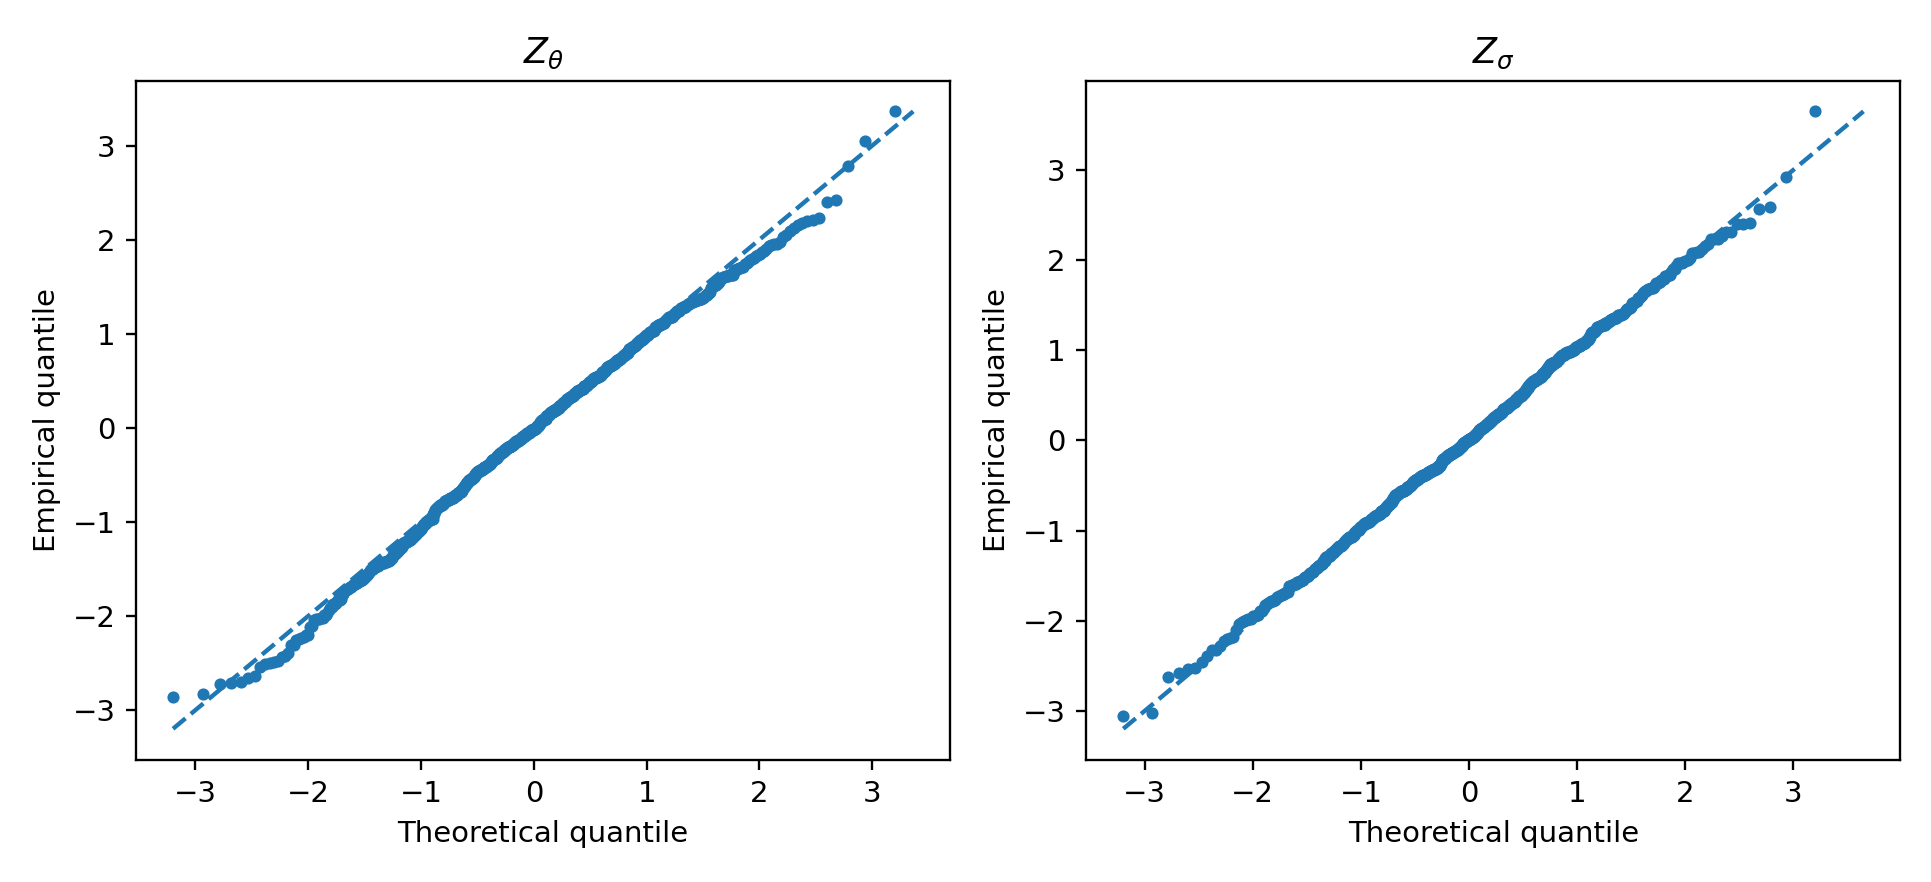
\includegraphics[width=.82\textwidth]{lan_qq_plots.png}
\caption{Normal quantile--quantile diagnostics for the standardised estimators. The visible right-skew of $Z_\theta$ at $N=5$ (skewness $0.49$, Kolmogorov--Smirnov $p=0.021$) dissipates along the design path ($p=0.42$ at $N=10$, $p=0.75$ at $N=20$), consistent with the first-order asymptotics.}
\label{fig:lan-qq}
\end{figure}

\subsection{Counterfactual process and bootstrap}

Fixed-intervention CDF sup-norm RMSE decreases from approximately $1.72\times10^{-3}$ to $2.13\times10^{-4}$. Distributional-effect sup-norm RMSE decreases from $1.64\times10^{-2}$ to $2.26\times10^{-3}$. Simultaneous coverage remains close to $0.95$ for both rate families.

\begin{table}[t]
\centering
\caption{Uniform target error and simultaneous coverage.}
\begin{tabular}{rrrrr}
\toprule
$N$ & CDF sup RMSE & Effect sup RMSE & Fast coverage & Slow coverage\\
\midrule
5  & $1.72\times10^{-3}$ & $1.64\times10^{-2}$ & 0.946 & 0.950\\
10 & $6.04\times10^{-4}$ & $6.29\times10^{-3}$ & 0.955 & 0.948\\
20 & $2.13\times10^{-4}$ & $2.26\times10^{-3}$ & 0.951 & 0.951\\
\bottomrule
\end{tabular}
\label{tab:coverage}
\end{table}

\begin{figure}[t]
\centering
\begin{subfigure}{.46\textwidth}
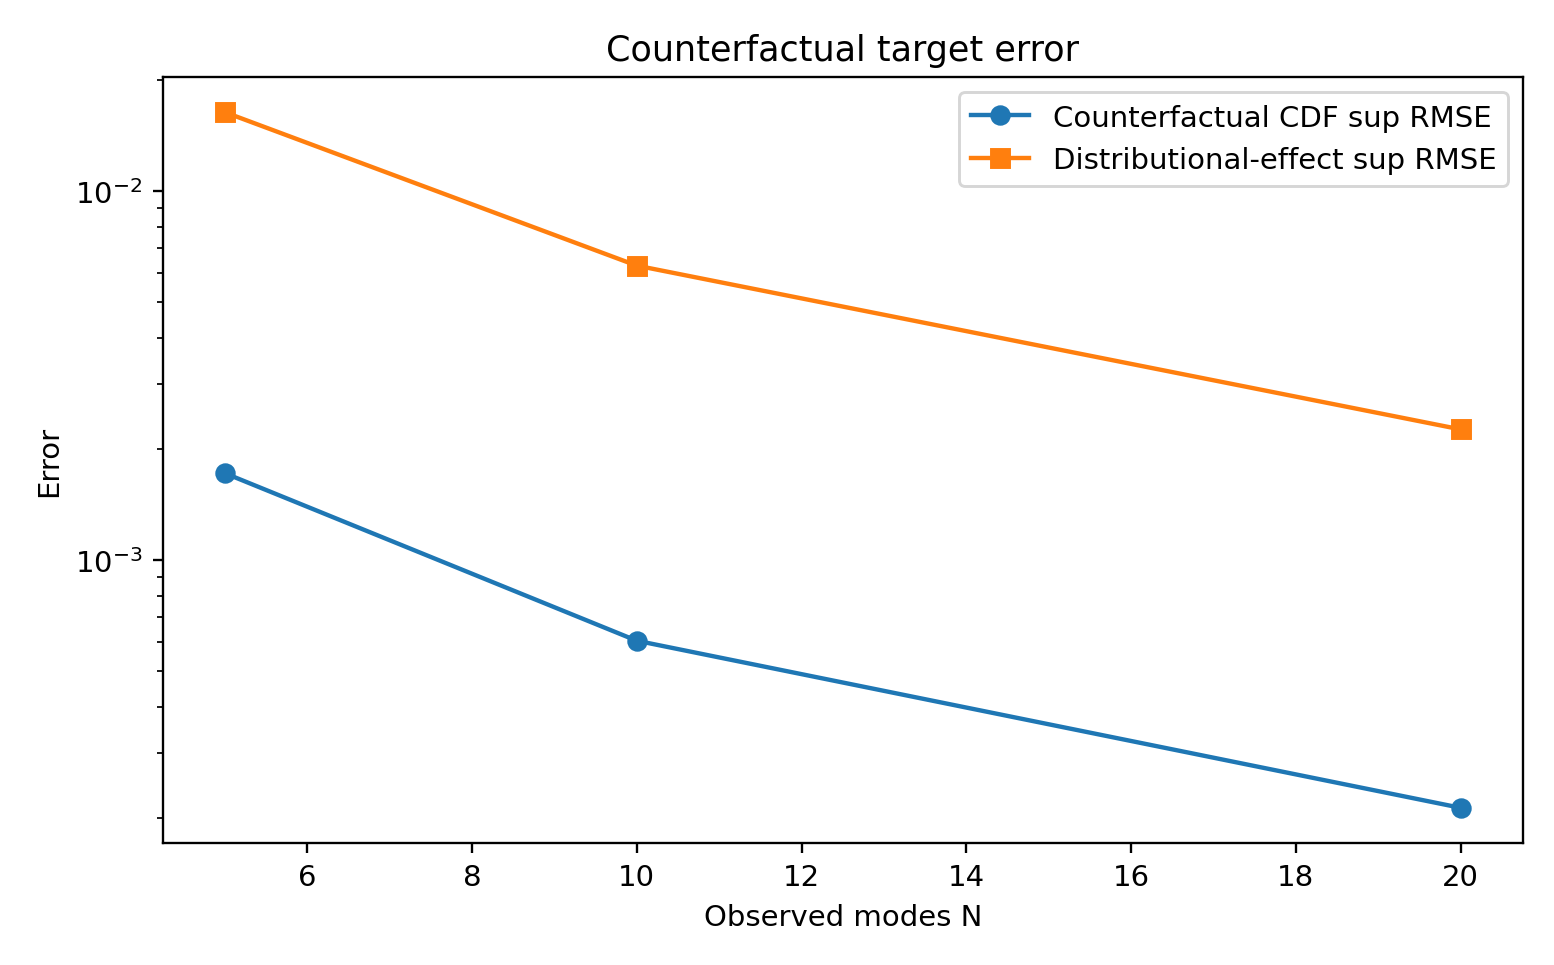
\includegraphics[width=\textwidth]{counterfactual_target_errors.png}
\caption{Uniform target errors.}
\end{subfigure}
\begin{subfigure}{.46\textwidth}
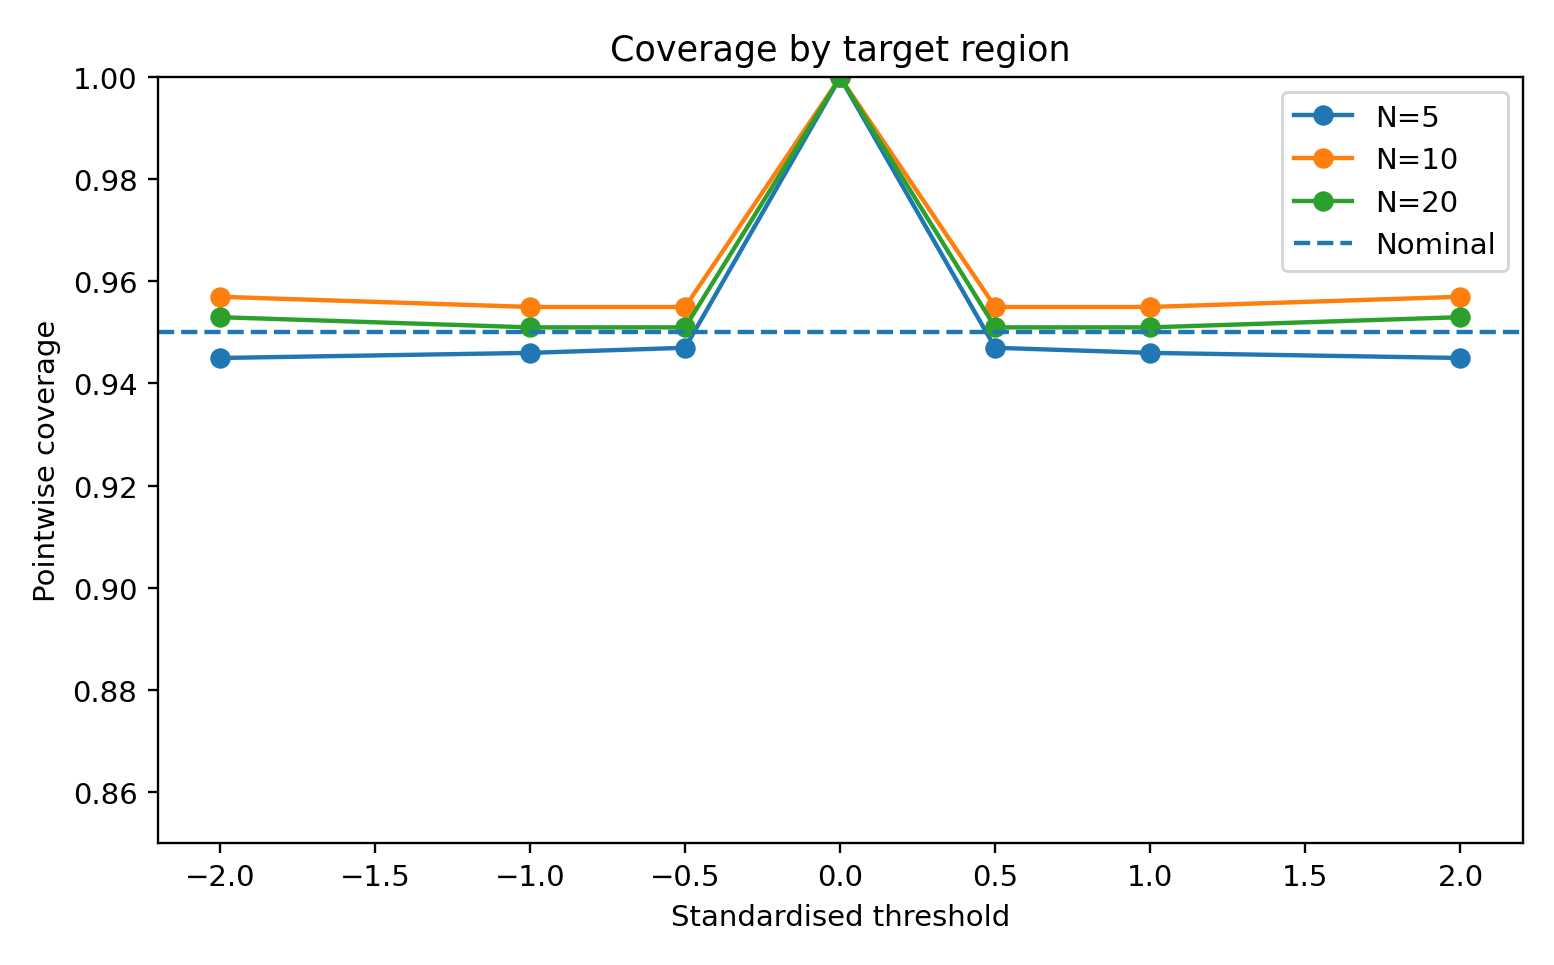
\includegraphics[width=\textwidth]{pointwise_coverage_by_threshold.png}
\caption{Coverage across thresholds.}
\end{subfigure}
\caption{Counterfactual target accuracy and coverage.}
\end{figure}

Beyond the headline coverage, the multiplier construction itself was stress-tested at $(N,n)=(10,8000)$ with $300$ replications per variant: the direct Gaussian draw, the modal-score multiplier with Gaussian weights, and the modal-score multiplier with Rademacher weights give statistically indistinguishable simultaneous coverage, and coverage is flat in the number of draws and in the threshold-grid resolution.

\begin{table}[t]
\centering
\caption{Bootstrap implementation sensitivity at $(N,n)=(10,8000)$, $300$ replications per row (Monte Carlo s.e.\ $\approx0.013$); nominal level $0.95$.}
\label{tab:boot-sens}
\begin{tabular}{llrrr}
\toprule
axis & variant & draws & fast cov. & slow cov.\\
\midrule
multiplier & direct Gaussian & 499 & 0.933 & 0.930\\
multiplier & modal Gaussian & 499 & 0.960 & 0.947\\
multiplier & modal Rademacher & 499 & 0.957 & 0.947\\
draws & direct Gaussian & 199 & 0.940 & 0.937\\
draws & direct Gaussian & 999 & 0.940 & 0.927\\
grid ($11$ pts) & direct Gaussian & 499 & 0.933 & 0.927\\
grid ($61$ pts) & direct Gaussian & 499 & 0.937 & 0.920\\
\bottomrule
\end{tabular}
\end{table}

\subsection{Approximation and sensitivity}

For the baseline spatial design, fitted log--log slopes are $-2.580$ for the mean tail, $-4.564$ for the variance tail, $-2.307$ for the strong RMS error, and $-2.580$ for the Gaussian CDF error, close to the theoretical values $-2.6,-4.6,-2.3,-2.6$. Temporal slopes lie between $0.994$ and $0.999$.

\begin{figure}[t]
\centering
\begin{subfigure}{.46\textwidth}
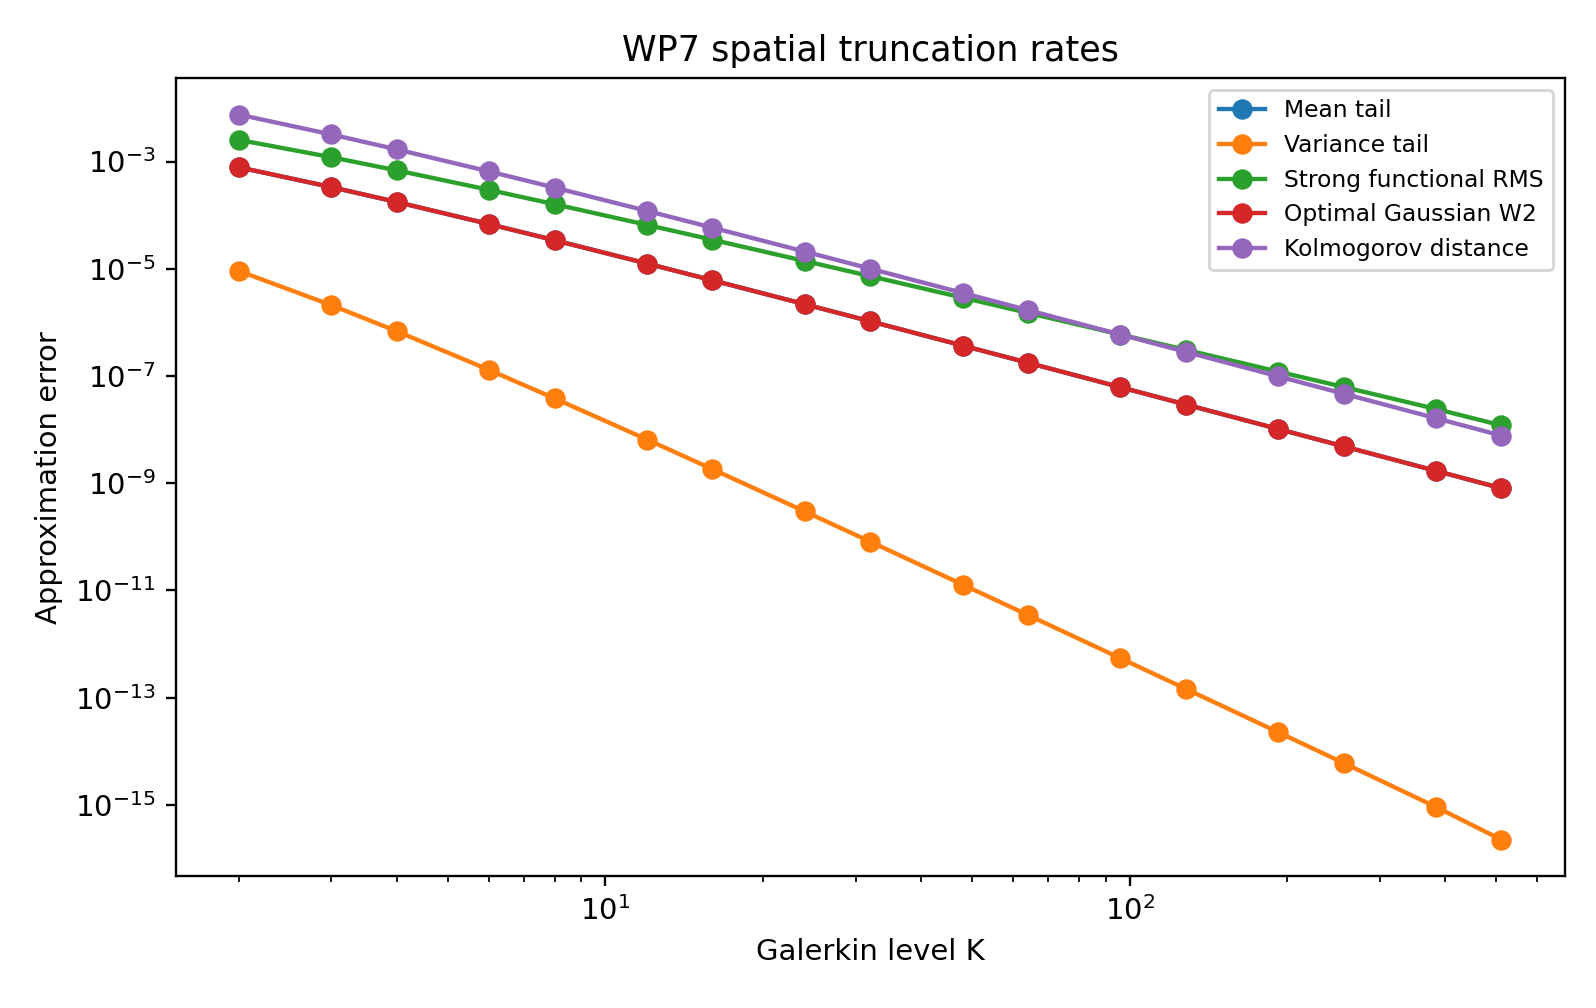
\includegraphics[width=\textwidth]{spatial_rates_baseline.png}
\caption{Galerkin rates.}
\end{subfigure}
\begin{subfigure}{.46\textwidth}
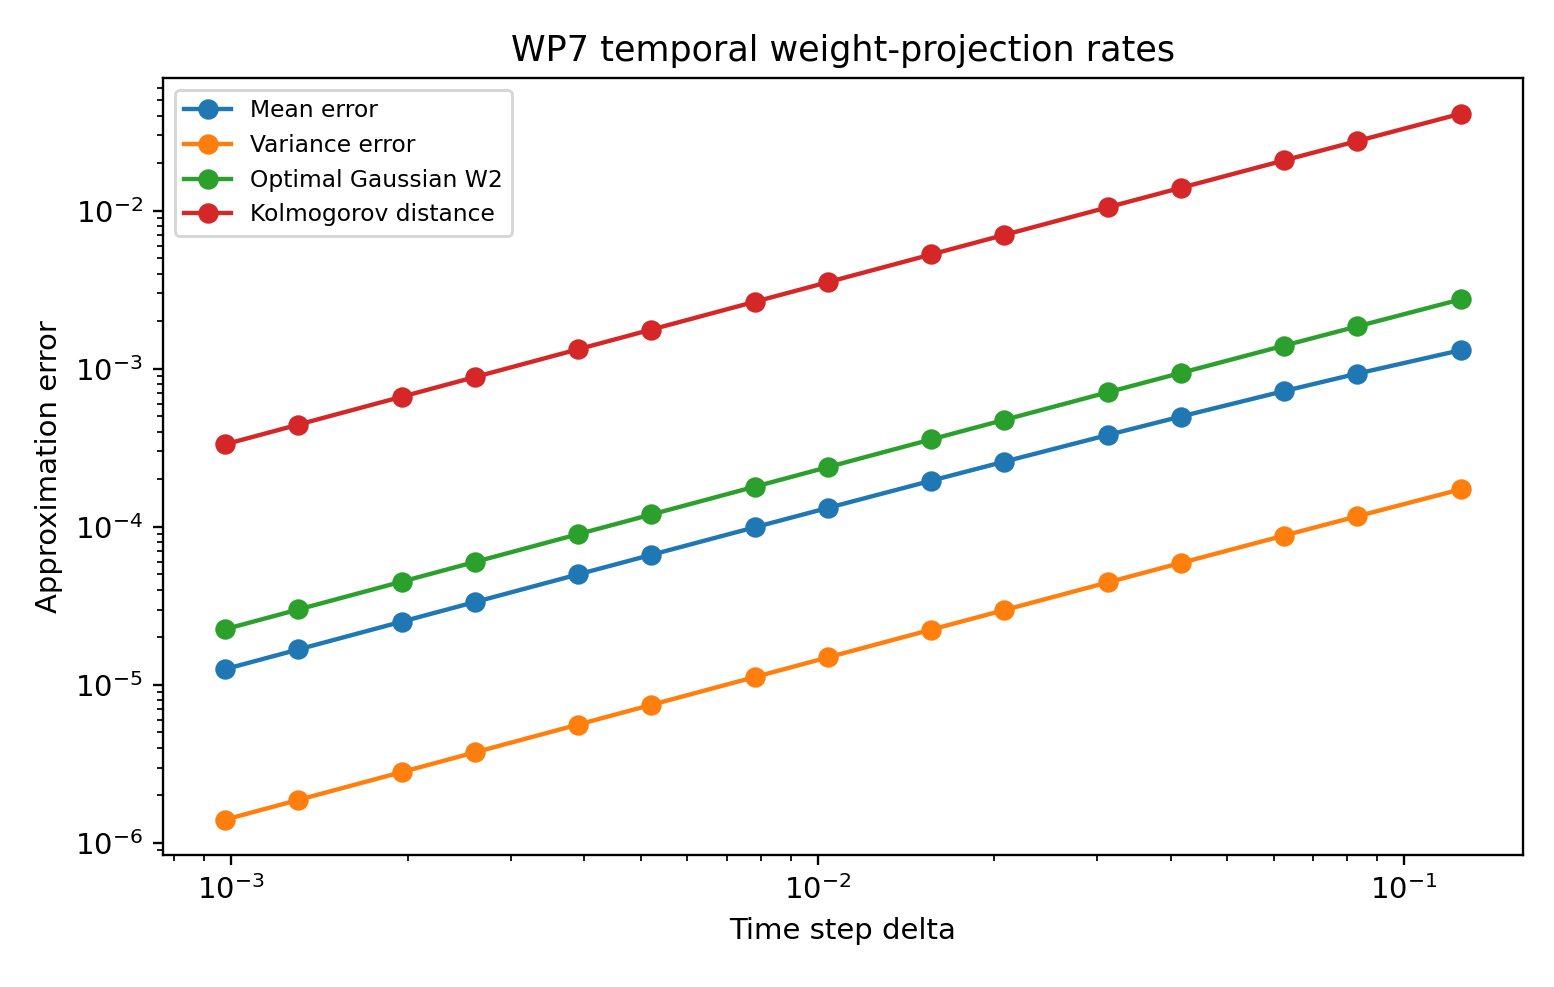
\includegraphics[width=\textwidth]{temporal_rates.png}
\caption{Temporal rates.}
\end{subfigure}
\caption{Deterministic approximation diagnostics.}
\end{figure}

For a non-commuting bounded perturbation, the central finite-difference derivative error decreases from $4.27\times10^{-6}$ at $\varepsilon=0.1$ to $1.71\times10^{-9}$ at $\varepsilon=0.002$. The CDF linearisation remainder is quadratic and the exact Gaussian $W_2$ distance remains below the derived Lipschitz envelope.

\subsection{Impossibility constructions}

The non-identification experiments are exact calculations rather than power studies. The adapted-feedback factual variance gap is zero while the post-intervention Kolmogorov distance is $0.0359$. The one-time open-loop factual variance gap is numerical zero and its post-intervention distance is $0.0984$. On a four-time grid, the factual covariance gap is $8.2\times10^{-16}$ while the post-intervention covariance gap is $0.7003$.


All tables and the headline diagnostics are regenerated by \texttt{make reproduce-publication}; the paper figures are regenerated end-to-end by the seeded validation pipeline (\texttt{make reproduce-paper}). The code records seeds, profiles, runtime, environment versions, and checksums.

\section{Discussion}

The paper places a narrow causal object on a complete mathematical and inferential footing. The intervention is an operator-module replacement inside a declared linear Gaussian SPDE class. The target is a counterfactual field-functional distribution. Identification is target specific. The inferential limit is mixed rate. Numerical approximation must be controlled at the target family's root-information scale.

Three distinctions are particularly important.

First, semantics and identification are separate. \Cref{sec:semantics} provides a coherent shared-noise intervention even before one asks whether the resulting law is recoverable from factual data; \Cref{sec:identification,sec:nonid} then characterise the positive and negative identification results.

Second, strong field approximation and Gaussian law approximation need not have the same rate. Under non-degeneracy, the variance tail enters normal CDF, quantile, and optimal Wasserstein comparisons linearly. Using the common-noise strong rate for every law target can be unnecessarily conservative.

Third, the phrase ``causal SPDE'' should not be read as unrestricted causal discovery. The intervention and invariant modules must be supplied. The feedback-gauge and open-loop constructions show that passive equality of factual laws cannot decide which part of a drift is the module that should be replaced.

Several extensions remain. Non-diagonal unbounded perturbations, including spatially varying divergence-form coefficients, require domain-sensitive perturbation theory. Semilinear equations require differentiability of nonlinear solution maps. Non-Gaussian noise calls for characteristic-function, Wasserstein, or quantile-specific methods rather than Gaussian mean--variance reduction. Physical-space observations require a separate statistical experiment and may produce different rates.

The present results are nevertheless sufficient for a coherent paper-level conclusion:
\begin{equation*}
\begin{aligned}
&\text{specified structural intervention}
+\text{identified factual experiment}\\
&\quad+\text{controlled numerical approximation}\\
&\hspace{2.5cm}\Longrightarrow
\text{uniformly inferable counterfactual laws}.
\end{aligned}
\end{equation*}
The impossibility results define the boundary of that conclusion rather than an exception to it.


\section*{Declarations}
\paragraph{Funding.} This work was supported by a DS4H (Digital Systems
for Humans) fellowship, Universit\'e C\^ote d'Azur.
\paragraph{Competing interests.} The author declares no competing interests.
\paragraph{Data and code availability.} All numerical results are generated
by the seeded replication package (Python reference implementation with a
Julia parity implementation, deterministic profiles, SHA-256 manifests, and
continuous-integration checks) archived with the manuscript sources; the
figures and tables of Section~\ref{sec:numerics} are reproduced end-to-end
by the documented \texttt{make} targets. [Repository DOI to be added upon
archival deposition.]
\paragraph{Acknowledgements.} Grammarly and generative AI tools were used
for proofreading, grammatical corrections, and targeted suggestions to
enhance sentence clarity. After using these tools, all authors reviewed and
edited the manuscript, taking full responsibility for its contents.

\bibliographystyle{plainnat}
\bibliography{references_merged}
\end{document}
